\chapter{Introduction}
Calorimeters are a key detector systems in high energy physics experiments
ranging from neutrino to particle collider detectors. In
particular, electromagnetic (EM) calorimeters are designed to fully
contain the energy deposisted by electrons, positrons, and photons (e/$\gamma$);
as well as to provide position information by means of their granular
design. They are usually divided in two types: homogeneous and
sampling, homogenous calorimeters are those in which their entire
volume is composed of sensitive media, while sampling calorimeters
are composed of alternating layers of sensitive and absorber
media. 

Homogeous EM calorimeters are usually made out of dense scintillating
crystals (BGO, BaF$_{2}$, LYSO, PbWO$_{4}$, among others) or liquid nobel gases
(Ar, Kr, Xe) and they provide an oustanding energy resolution for
e/$\gamma$. For example, the CMS EM calorimeter~\cite{cmsECAL} is
composed of PbWO$_{4}$ scintillating crystals coupled to avalance
photodiodes and with and energy resolution of

\begin{equation}
\frac{\sigma_{E}}{E} = \frac{2.8\%\sqrt{\GeV}}{\sqrt{E}} \oplus \frac{12\%\GeV}{E} \oplus 0.3\%.
\end{equation}

Sampling EM calorimeters use a sensitive medium such as
scintillating crystals, liquid nobel gases, and silicon, among others
to measure the energy the incoming particle;
while the absorber medium is a high density material such as lead or
tungsten in order to require less volume to completely contain the
impinging particle's energy and thus result in a compact design. An
example of such an EM calorimeter is the ATLAS lead-liquid argon (LAr)
sampling calorimeter with an energy resolution of

\begin{equation}
\frac{\sigma_{E}}{E} = \frac{10.1\%\sqrt{\GeV}}{\sqrt{E}} \oplus \frac{0.25\%\GeV}{E} \oplus 0.17\%.
\end{equation}

Particle collider experiments at the LHC such as ATLAS and CMS
use EM calorimeters in the e/$\gamma$ four-momentum and jet
energy measurements, particle identification algorithms,
trigger systems, and the mesurement of the missing transverse energy in
each proton-proton collision. Therefore, maintaining the current perfomance of the EM
calorimeters is critical for the current and future physics measurements of those experiments.

In order to provide the necessary datasets to perform precision measurements of the Higgs couplings, 
probe rare Higgs processes, study the scattering of longitudinally polarized W
bosons, and search for new physics. The high luminosity upgrade of the Large Hadron Collider (HL-LHC) at
CERN~\cite{Rossi:1471000} is expected to provide instantaneous luminosities of
$5\times10^{34}$ cm$^{-2}$s$^{-1}$. This enhanced data rate will
increase the simultaneous interactions per bunch crossing (pileup)
from an average of $20$-$40$ to $140$-$200$. 

The large amount of pileup foreseen for the HL-LHC will increases the likelihood of 
confusion in the reconstruction of events of interest, due to the contamination from 
particles produced in different pileup interactions. The ability to discriminate between 
jets produced in the events of interests -- especially those associated with the vector 
boson fusion processes -- and jets produced by pileup interactions will be degraded, 
the missing transverse energy resolution will deteriorate, and several other physics 
objects performance metrics will suffer.

One way to mitigate the detrimental pileup effects, complementary to precision tracking methods, 
is to perform a time of arrival measurement associated with a particular layer of the calorimeter, 
allowing for a time assignment for both charged particles and photons. Such a measurement with 
a precision of about $20$ to $30$~ps, when unambiguously associated to the corresponding energy
measurement, will significantly reduce -- approximately a factor of 10
-- the inclusion of pileup particles in the
reconstruction of the event of interest given that the spread in collision time of
pileup interactions is about $200$~ps. The association of the time measurement to the energy 
measurement is crucial,  leading to  a  prototype  design that requires the time and energy 
measurements to be performed in the same sensitive medium. It is in
this context that this thesis presents various prototype
calorimeters equipped with precision timing capabilities and studies the current limits on their time resolution.

This part of the thesis is organized as follows: section~\ref{prelim-cal}
provides a brief and general introduction to EM calorimeters, chapter~\ref{lyso-cal} is
dedicated to the timing properties of LYSO crystal scintillator based
calorimeters, chapter~\ref{mcp-cal} discusses the possibility of a precision timing sampling
calorimeter where the sensitive medium is a microchannel
plate (MCP)~\cite[MCP], chapter~\ref{sil-cal} discusses the timing capabilities of a sampling
calorimeter where the sensitive medium is a 350 microns silicon
sensor. finally, chapter~\ref{cal-sum} summarizes the results and
possible improvements as well as future measurements.
\section{EM Calorimeter Preliminaries}\label{prelim-cal}
Calorimeters are highly complex instruments and therefore some
background is required to understand the subsequent sections in this
chater; this section is intended to provide a short overview of the
most important effects -- mostly different physical processes in
different energy regimes -- and the relevant considerations when
designing a calorimeter.
\subsection{EM Shower Development}
High energy e/$\gamma$ (with energies above 1\GeV) will develop an EM
shower upon entering the calorimeter. The processes involved in the EM
shower development are few and well understood. Photons lose energy
mostly by photoelectric effect, Compton scattering, or pair production
of electrons and positrons. The later dominates at high energies and
it is reponsible for the shower development, while
photoelectric effect overwhelmingly dominates at low energies
(typically below ~10\MeV), Figure~\ref{fig:photonEL} shows the photon cross
section as a function of the incoming photon energy in lead.
\begin{figure}[h] \centering
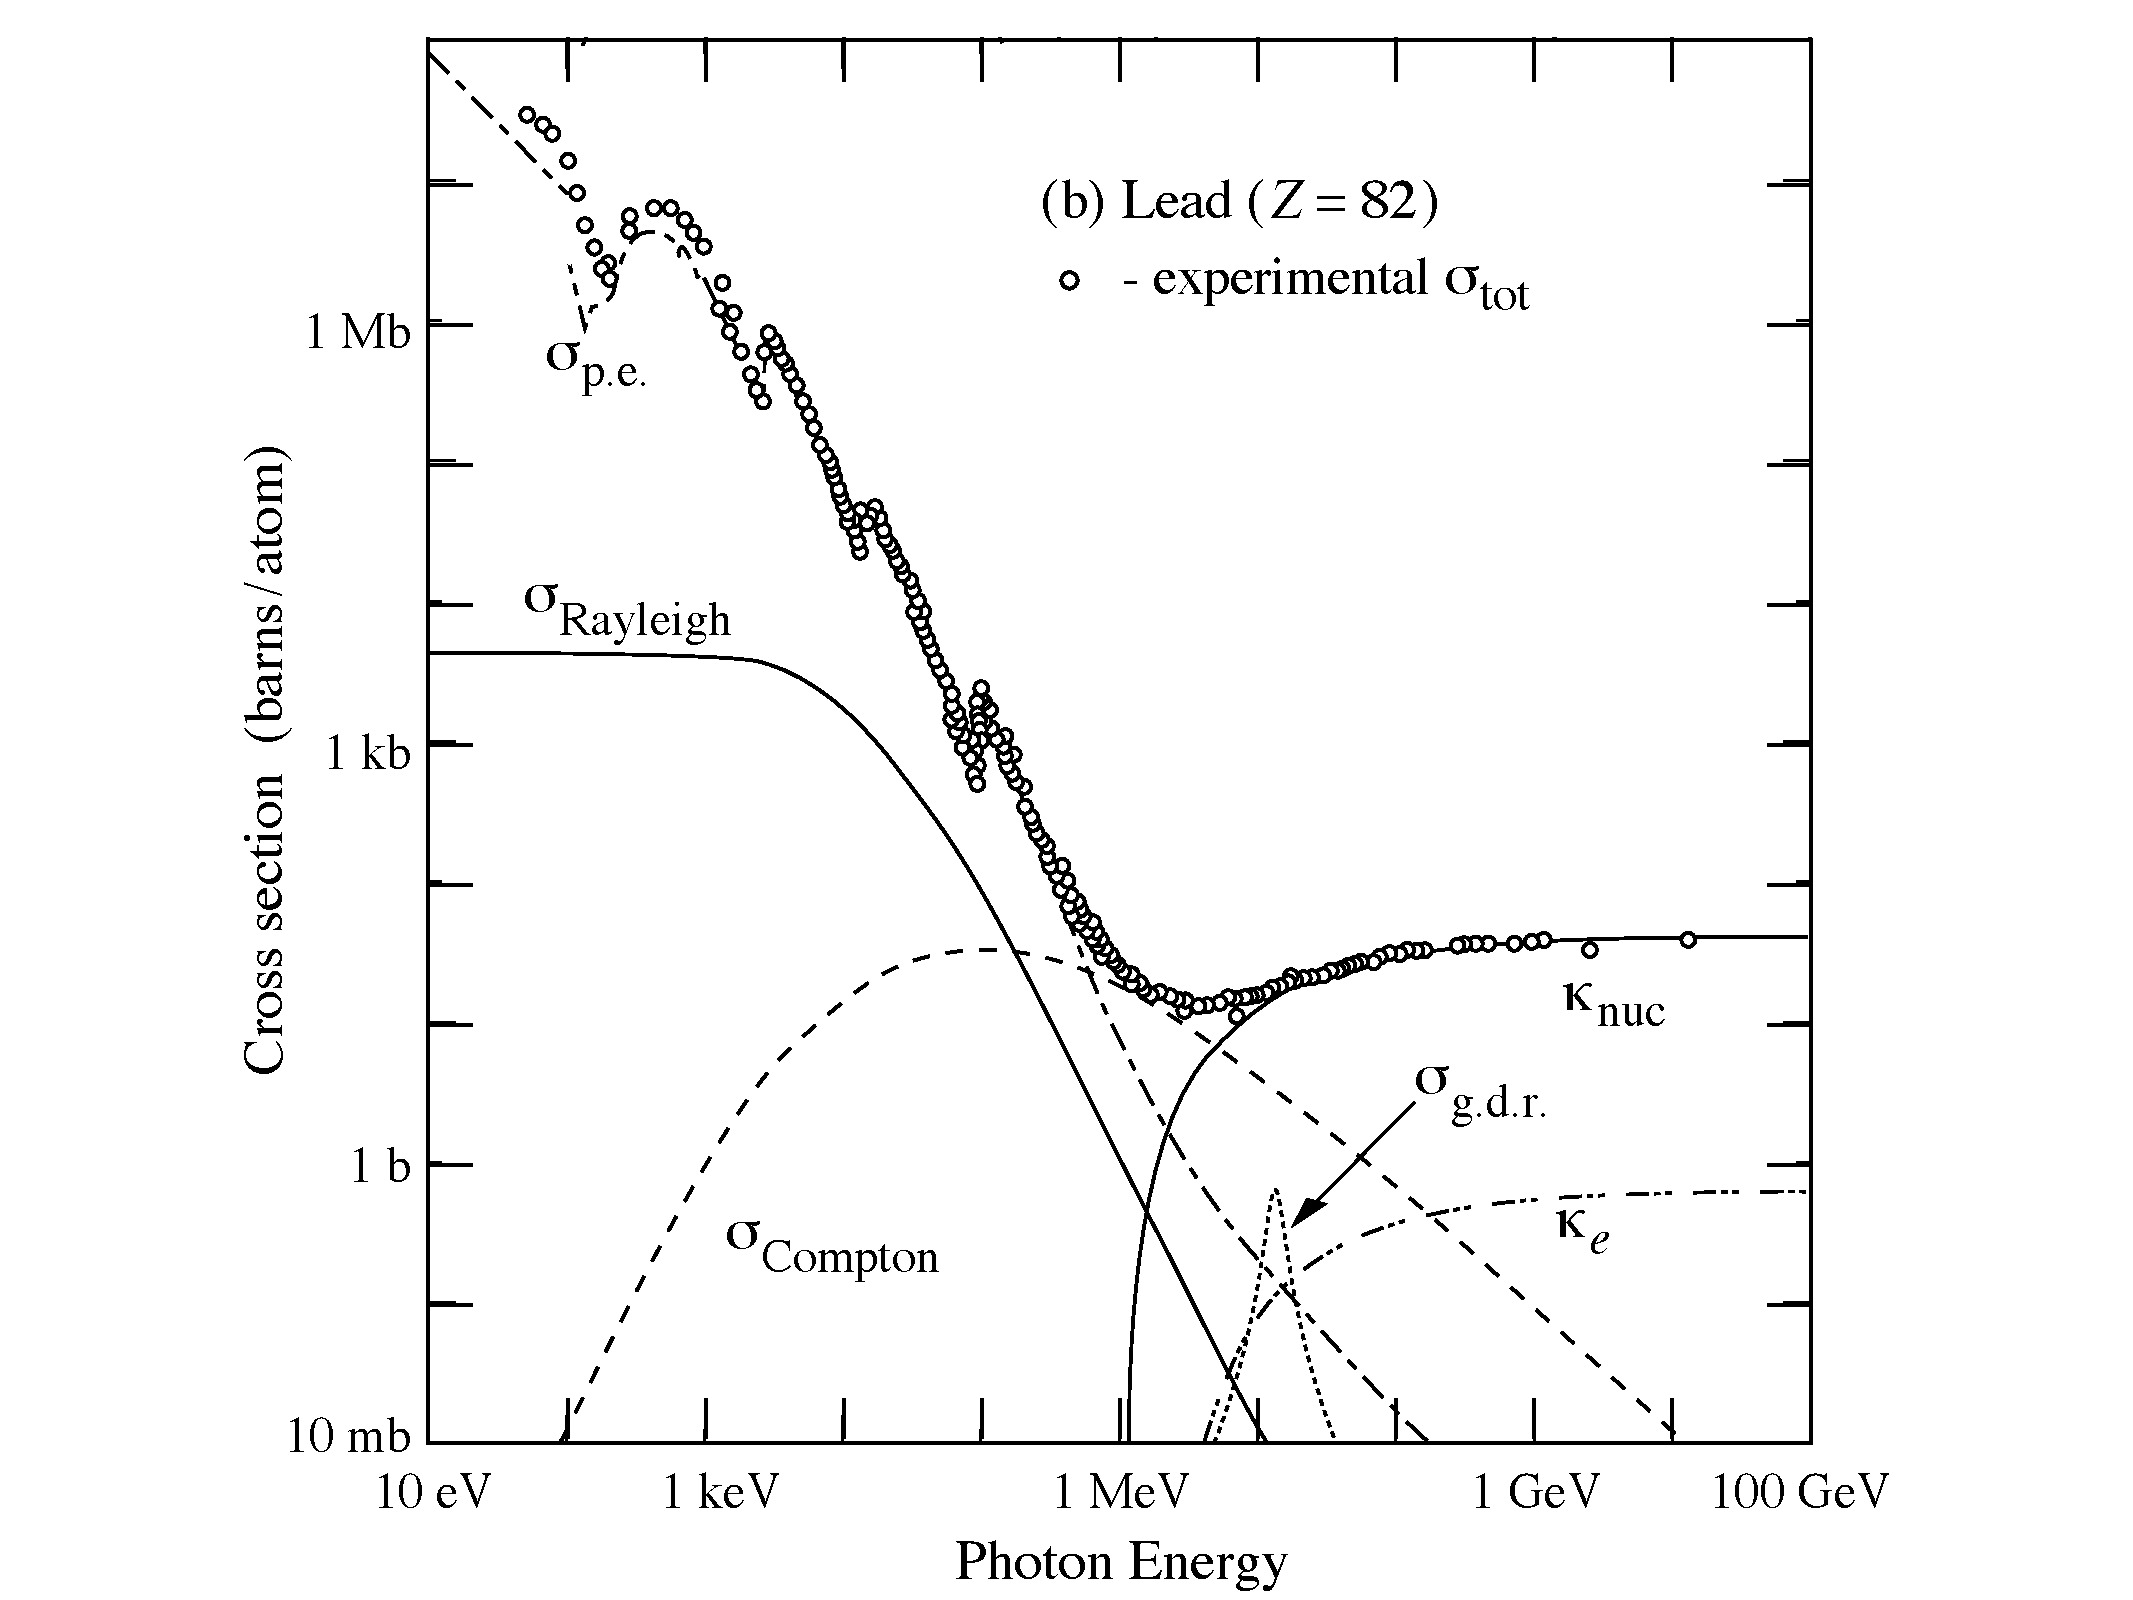
\includegraphics[width=0.85\textwidth]{calorimetry/PhotonXsec.pdf}
\caption{Cross
section as a function of the incoming photon energy in lead.}
\label{fig:photonEL}
\end{figure} 
Electrons and positrons lose energy mainly due to two processes,
ionization and radiation hereafter refer to as bremsstrahlung, see Figure~\ref{fig:electronEL}. The
later dominates at high energies while the former dominates at low
energies. The energy at which these two processes are equally relevant
is defined as the critical energy ($E_{c}$)~\cite{criticalE}, Figure~\ref{fig:criticalE}
shows a graphical representation of this definition.
\begin{figure}[h] \centering
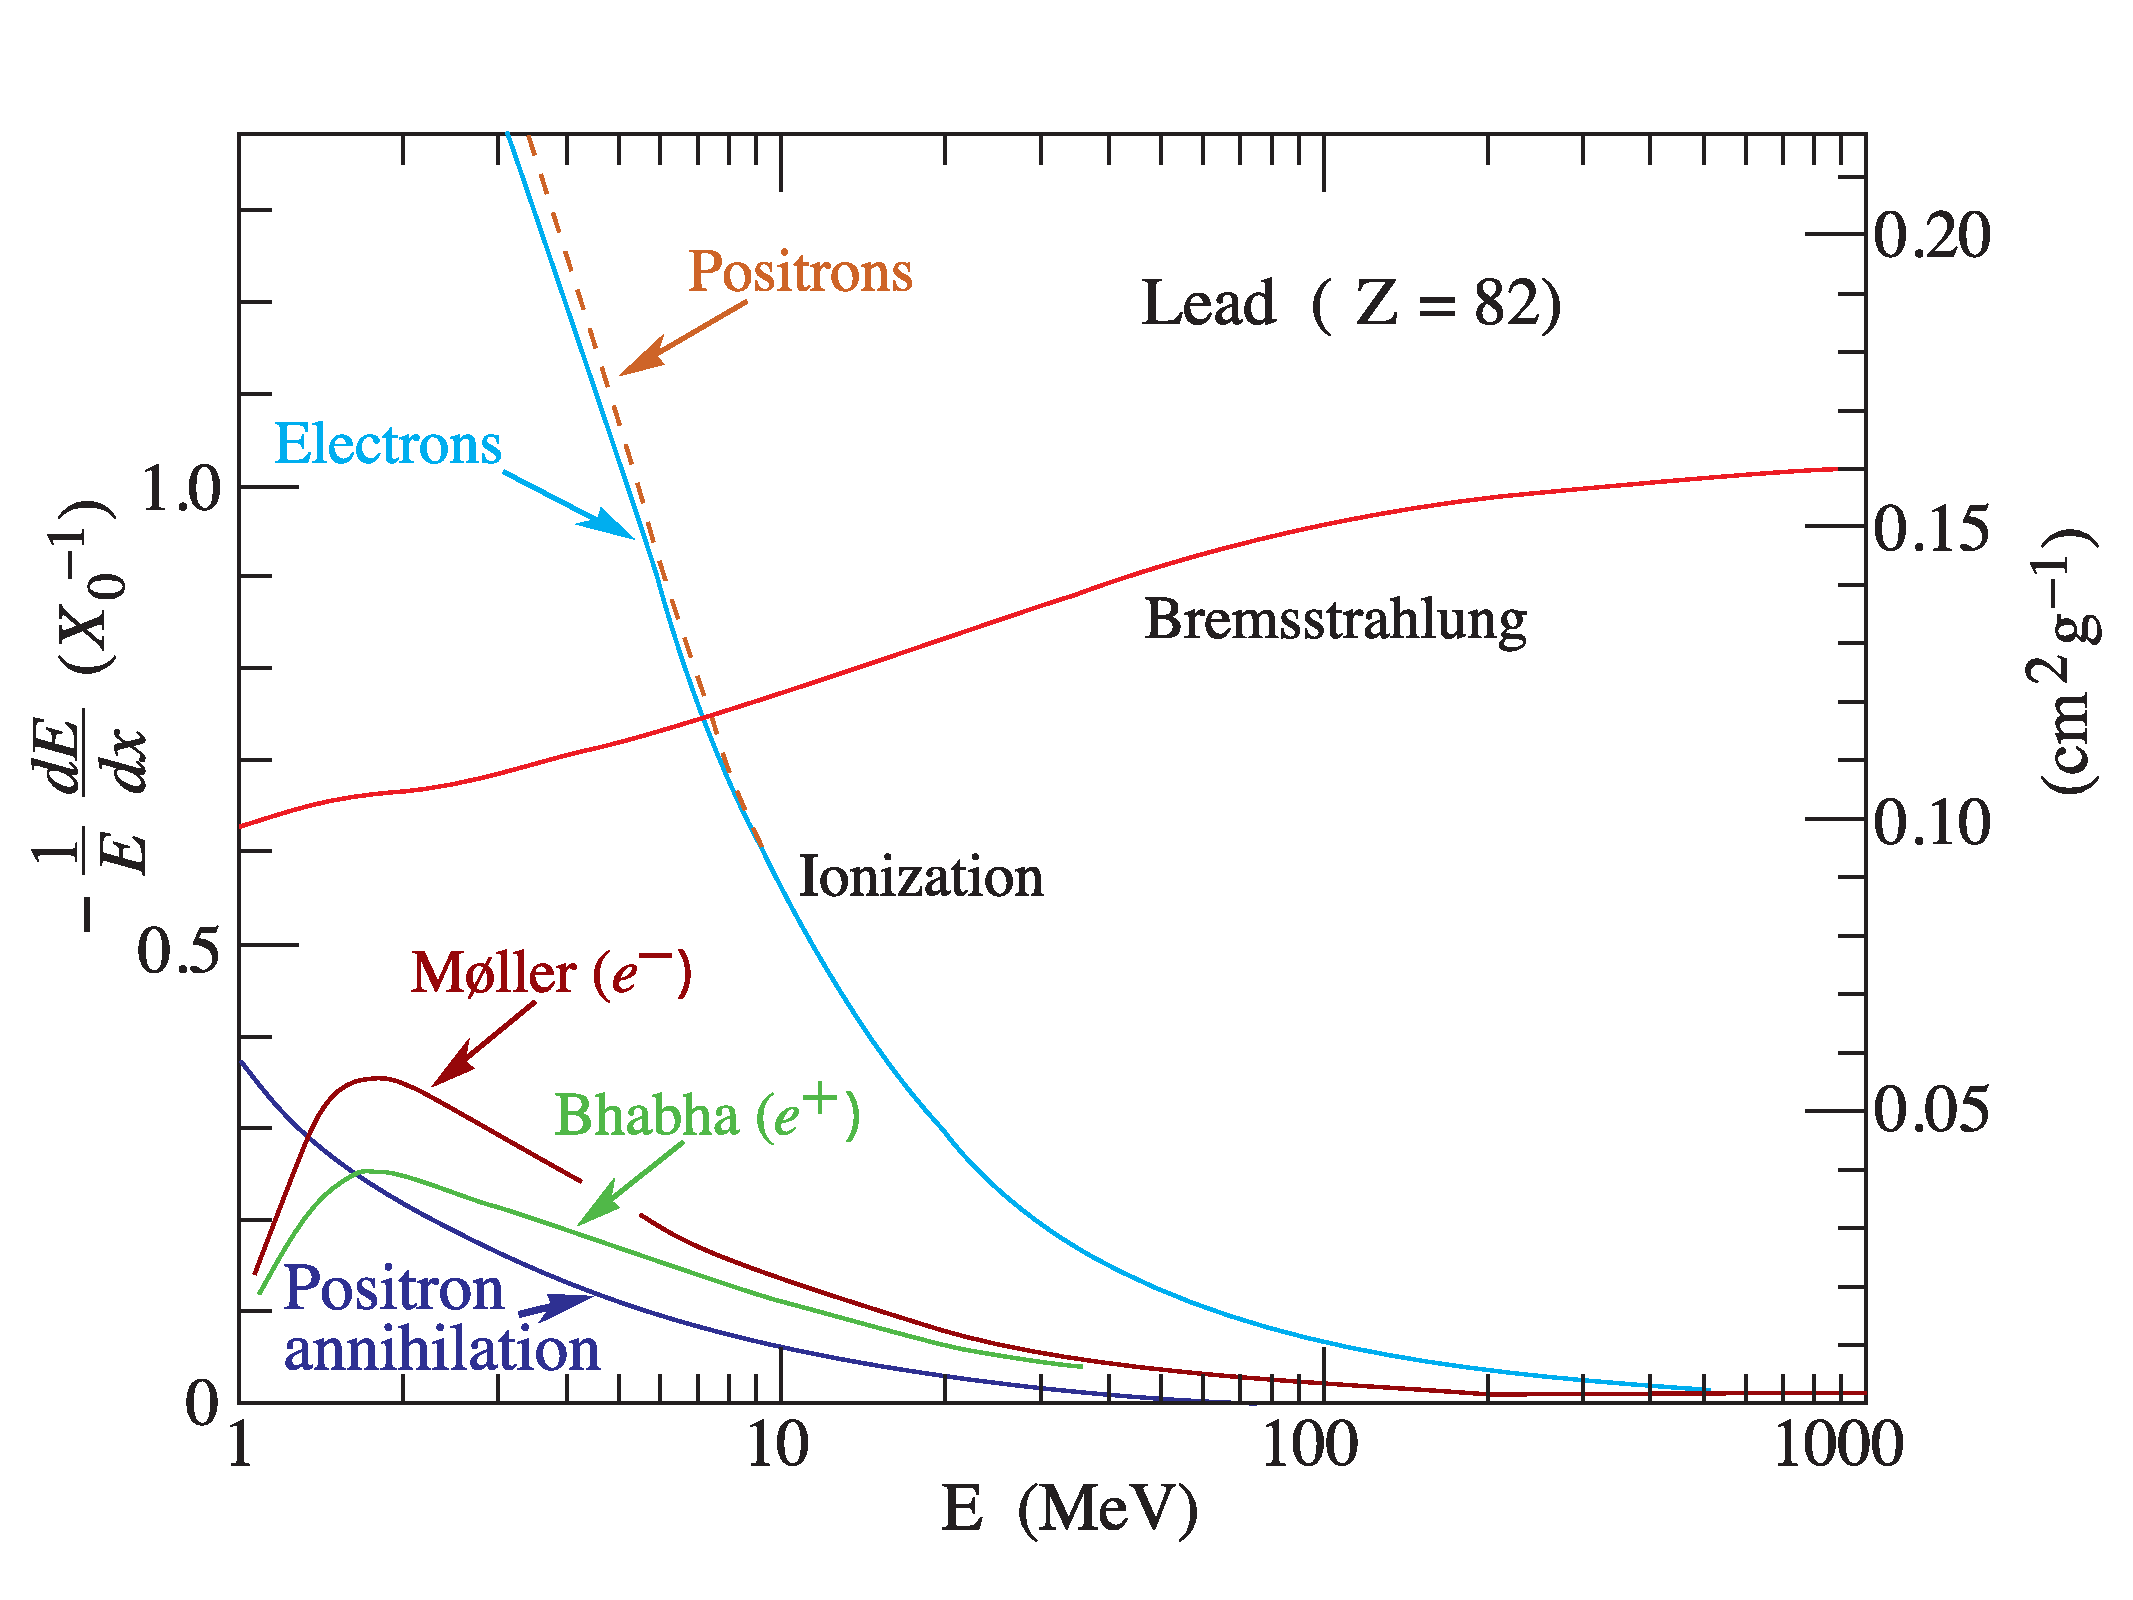
\includegraphics[width=0.85\textwidth]{calorimetry/dEdx_electrons.pdf}
\caption{Fractional energy loss per radiation
  length in lead as a function of the electron/positron energy.}
\label{fig:electronEL}
\end{figure} 

\begin{figure}[h] \centering
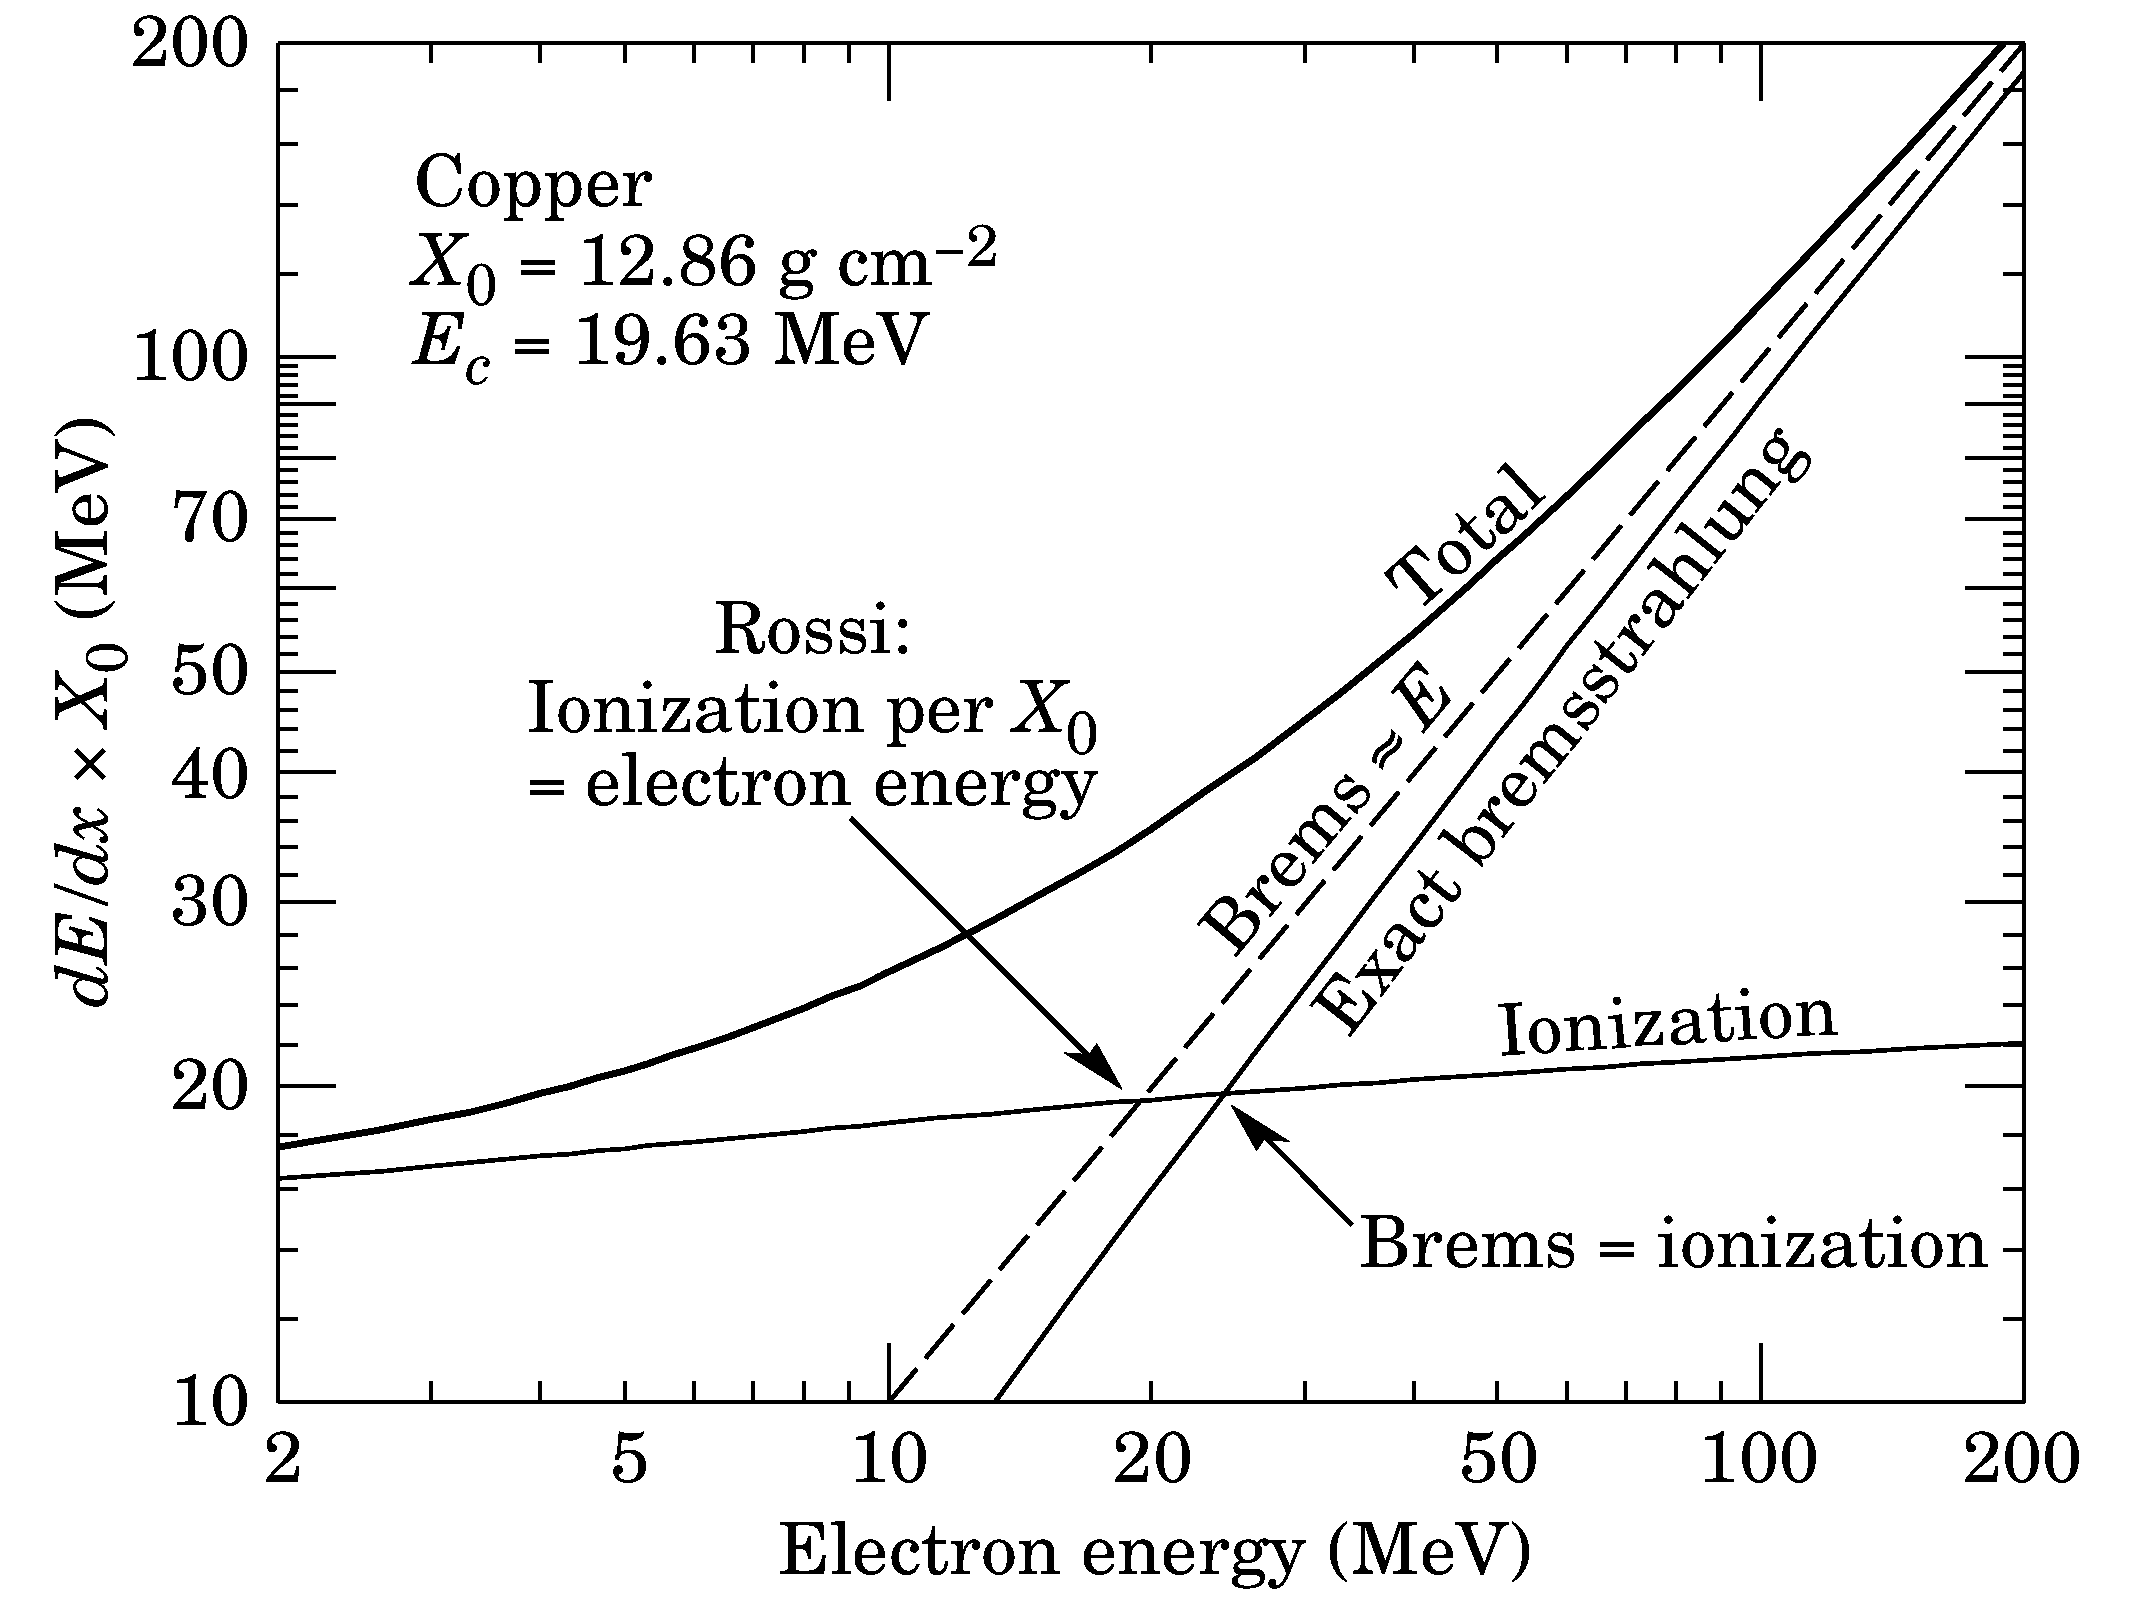
\includegraphics[width=0.85\textwidth]{calorimetry/CriticalEnergyDefinition.pdf}
\caption{Graphical definition of the critical energy ($E_{c}$). The
  intersection of the solid lines is the definition used in this
  thesis. The intersection between the solid (ionization) and dashed
  line is alternative definition.}
\label{fig:criticalE}
\end{figure} 
Empirical functional forms for $E_{c}$ can be obtained when a
distinction between gase and liquid or solid media is made, since there are
significant difference in ionization that arise mainly due to the
density effect. Figure~\ref{fig:criticalEFF} shows the experimental
data for $E_{c}$ as a function of the atomic number (Z) along with the
corresponding fits, the functional forms for $E_{c}$ are
\begin{equation}
E^{gas}_{c} = \frac{710\MeV}{Z+0.92}\mathrm{,}\hspace{0.5cm}\mathrm{and}\hspace{0.5cm}E^{solid}_{c} = \frac{610\MeV}{Z+1.24}.
\end{equation}

\begin{figure}[h] \centering
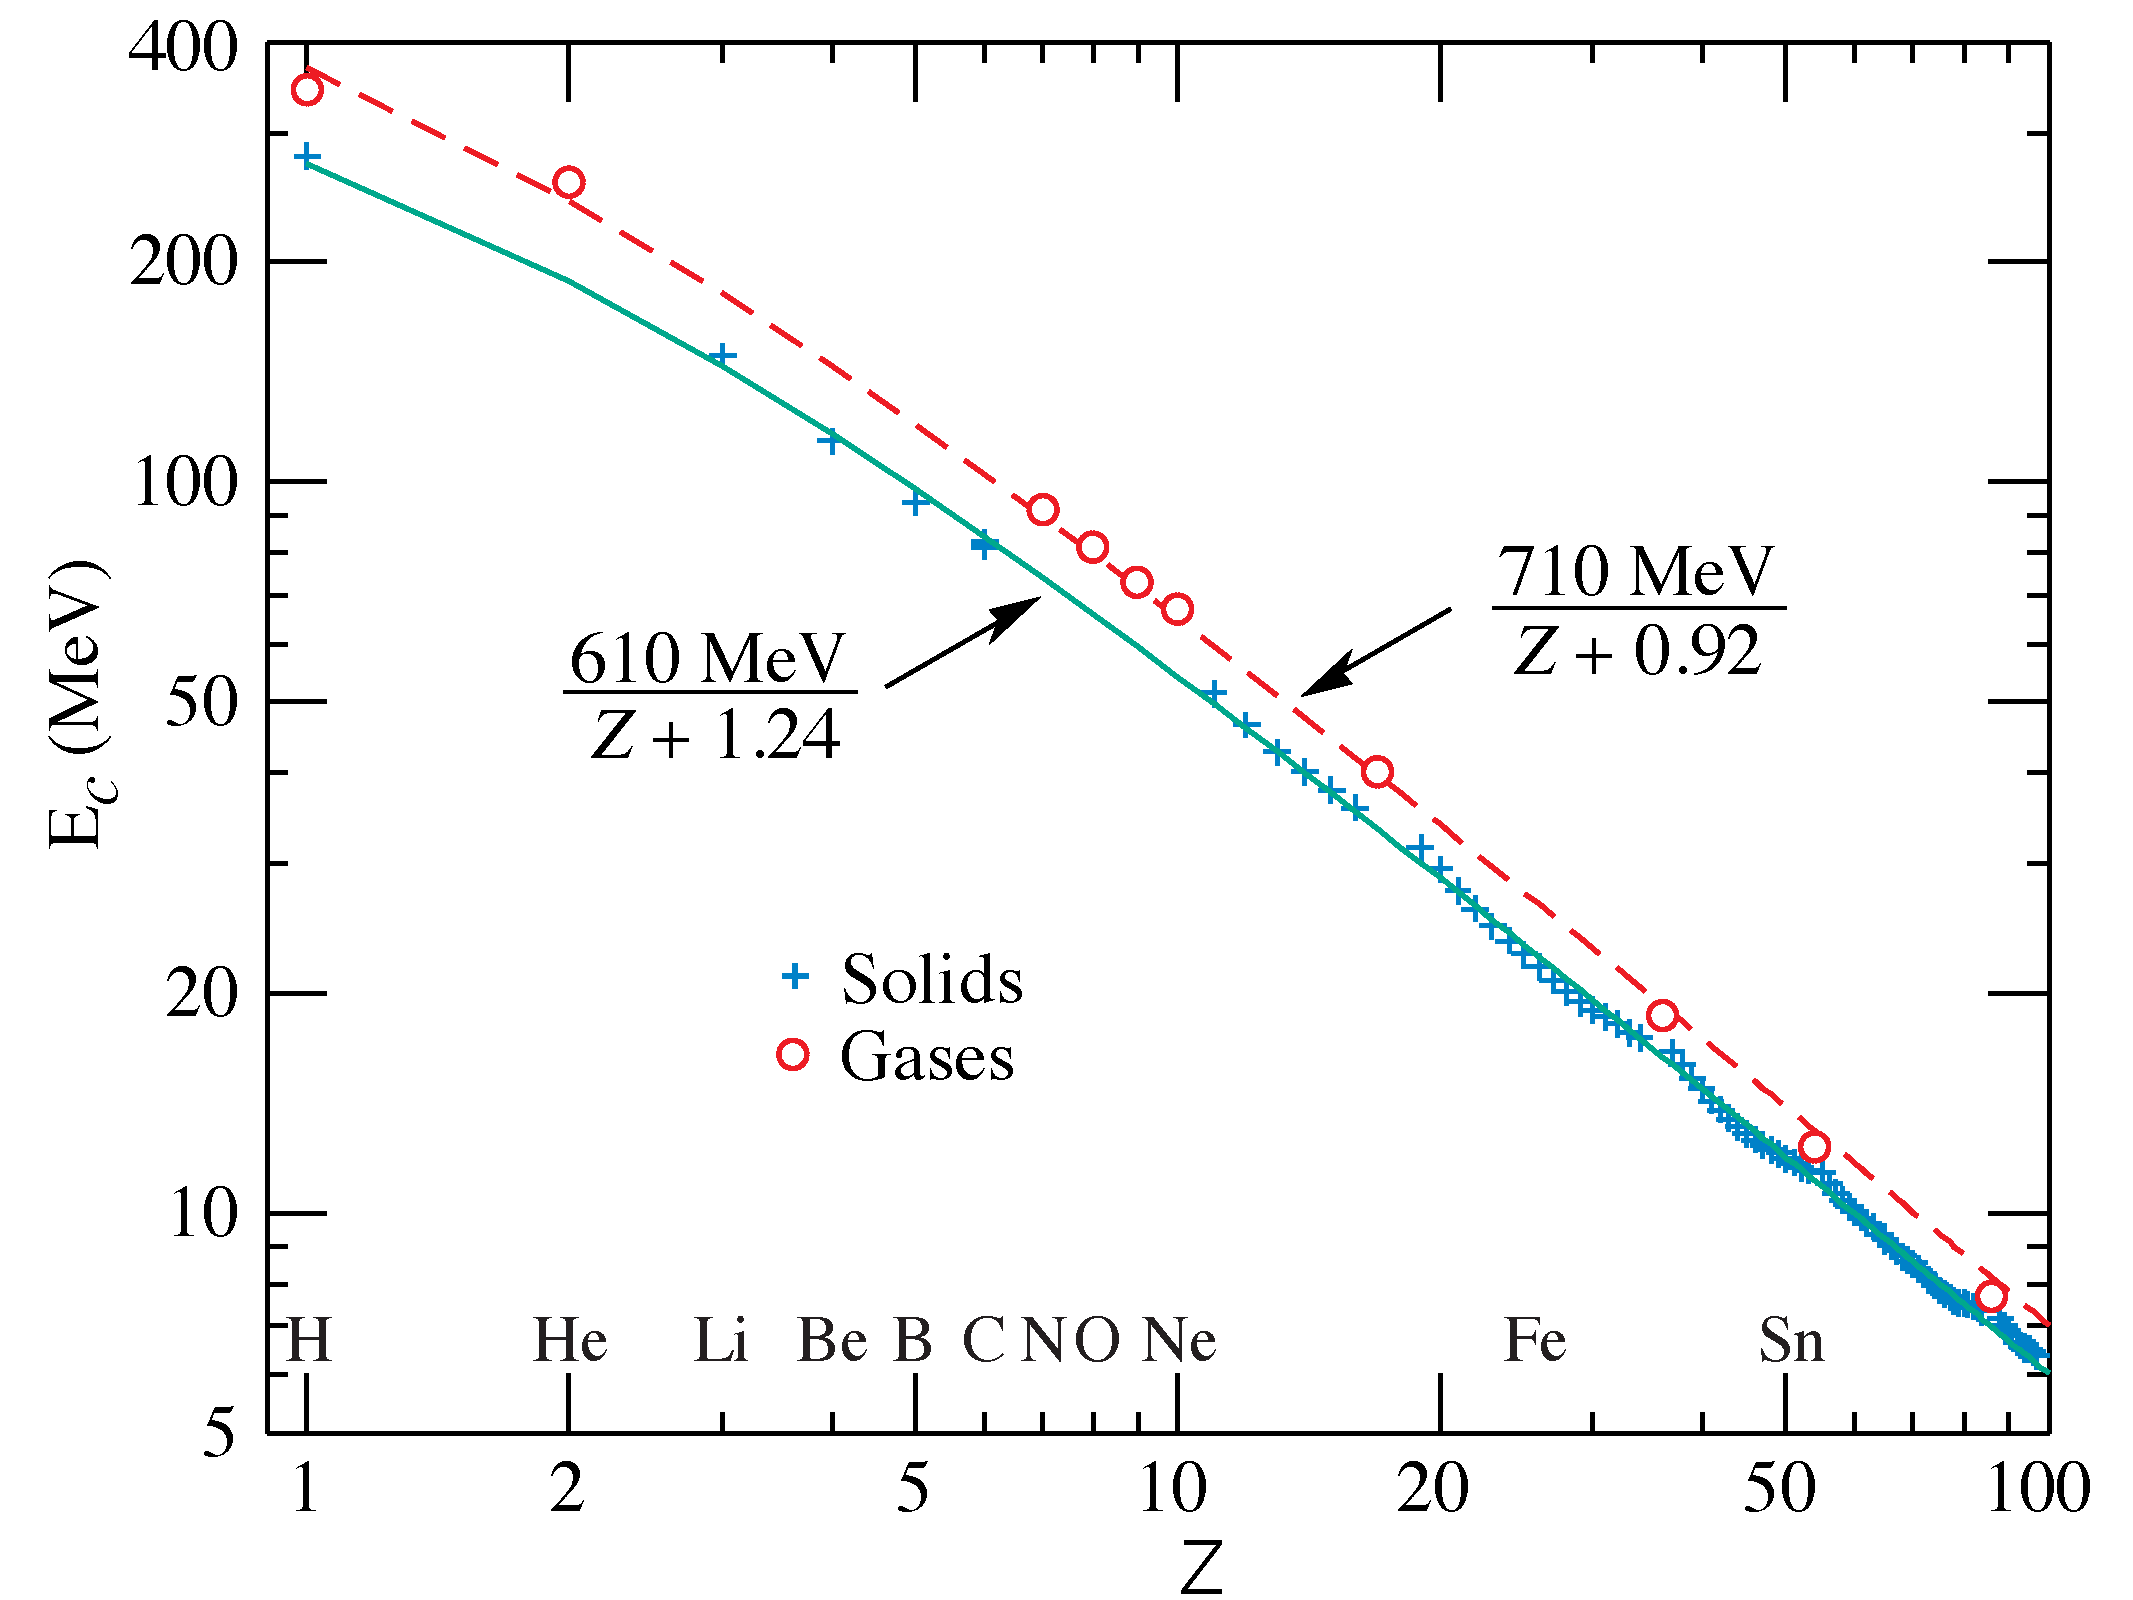
\includegraphics[width=0.85\textwidth]{calorimetry/CriticalEnergy.pdf}
\caption{Electron critical energy ($E_{c}$) for the chemical
  elements. Experimental data is shown for gases (red circles) and
  solids (magenta crosses). Fits are shown for gases (dashed red line)
and solids (solid magenta line)}
\label{fig:criticalEFF}
\end{figure} 

EM showers are then produced when high energy photons
(electron/positron) enters the calorimeter media and loses energy by
pair production (bremsstrahlung), the subsequently $e^{+}$/$e^{-}$
pair (high energy photon produced by radiation) loses energy by
bremsstralung (pair production). The number of particles produced by
this multiplicative process increases until a maximum is reached
(shower maximum) at the certain depth inside the calorimeter. After
this point the newly created particles have low energies and therefore other processes such as
photoelectric effect, Compton scatterring, and ionization start to
become relevant. The shower profile in the longitudinal direction for
a 30\GeV electron in iron is
shown in Figure~\ref{fig:showerProfile1}. The longitudinal shower
profile is also a function of the incoming particle energy,
Figure~\ref{fig:showerProfile1} shows this effect for electrons of
different energies in copper.

\begin{figure}[h] \centering
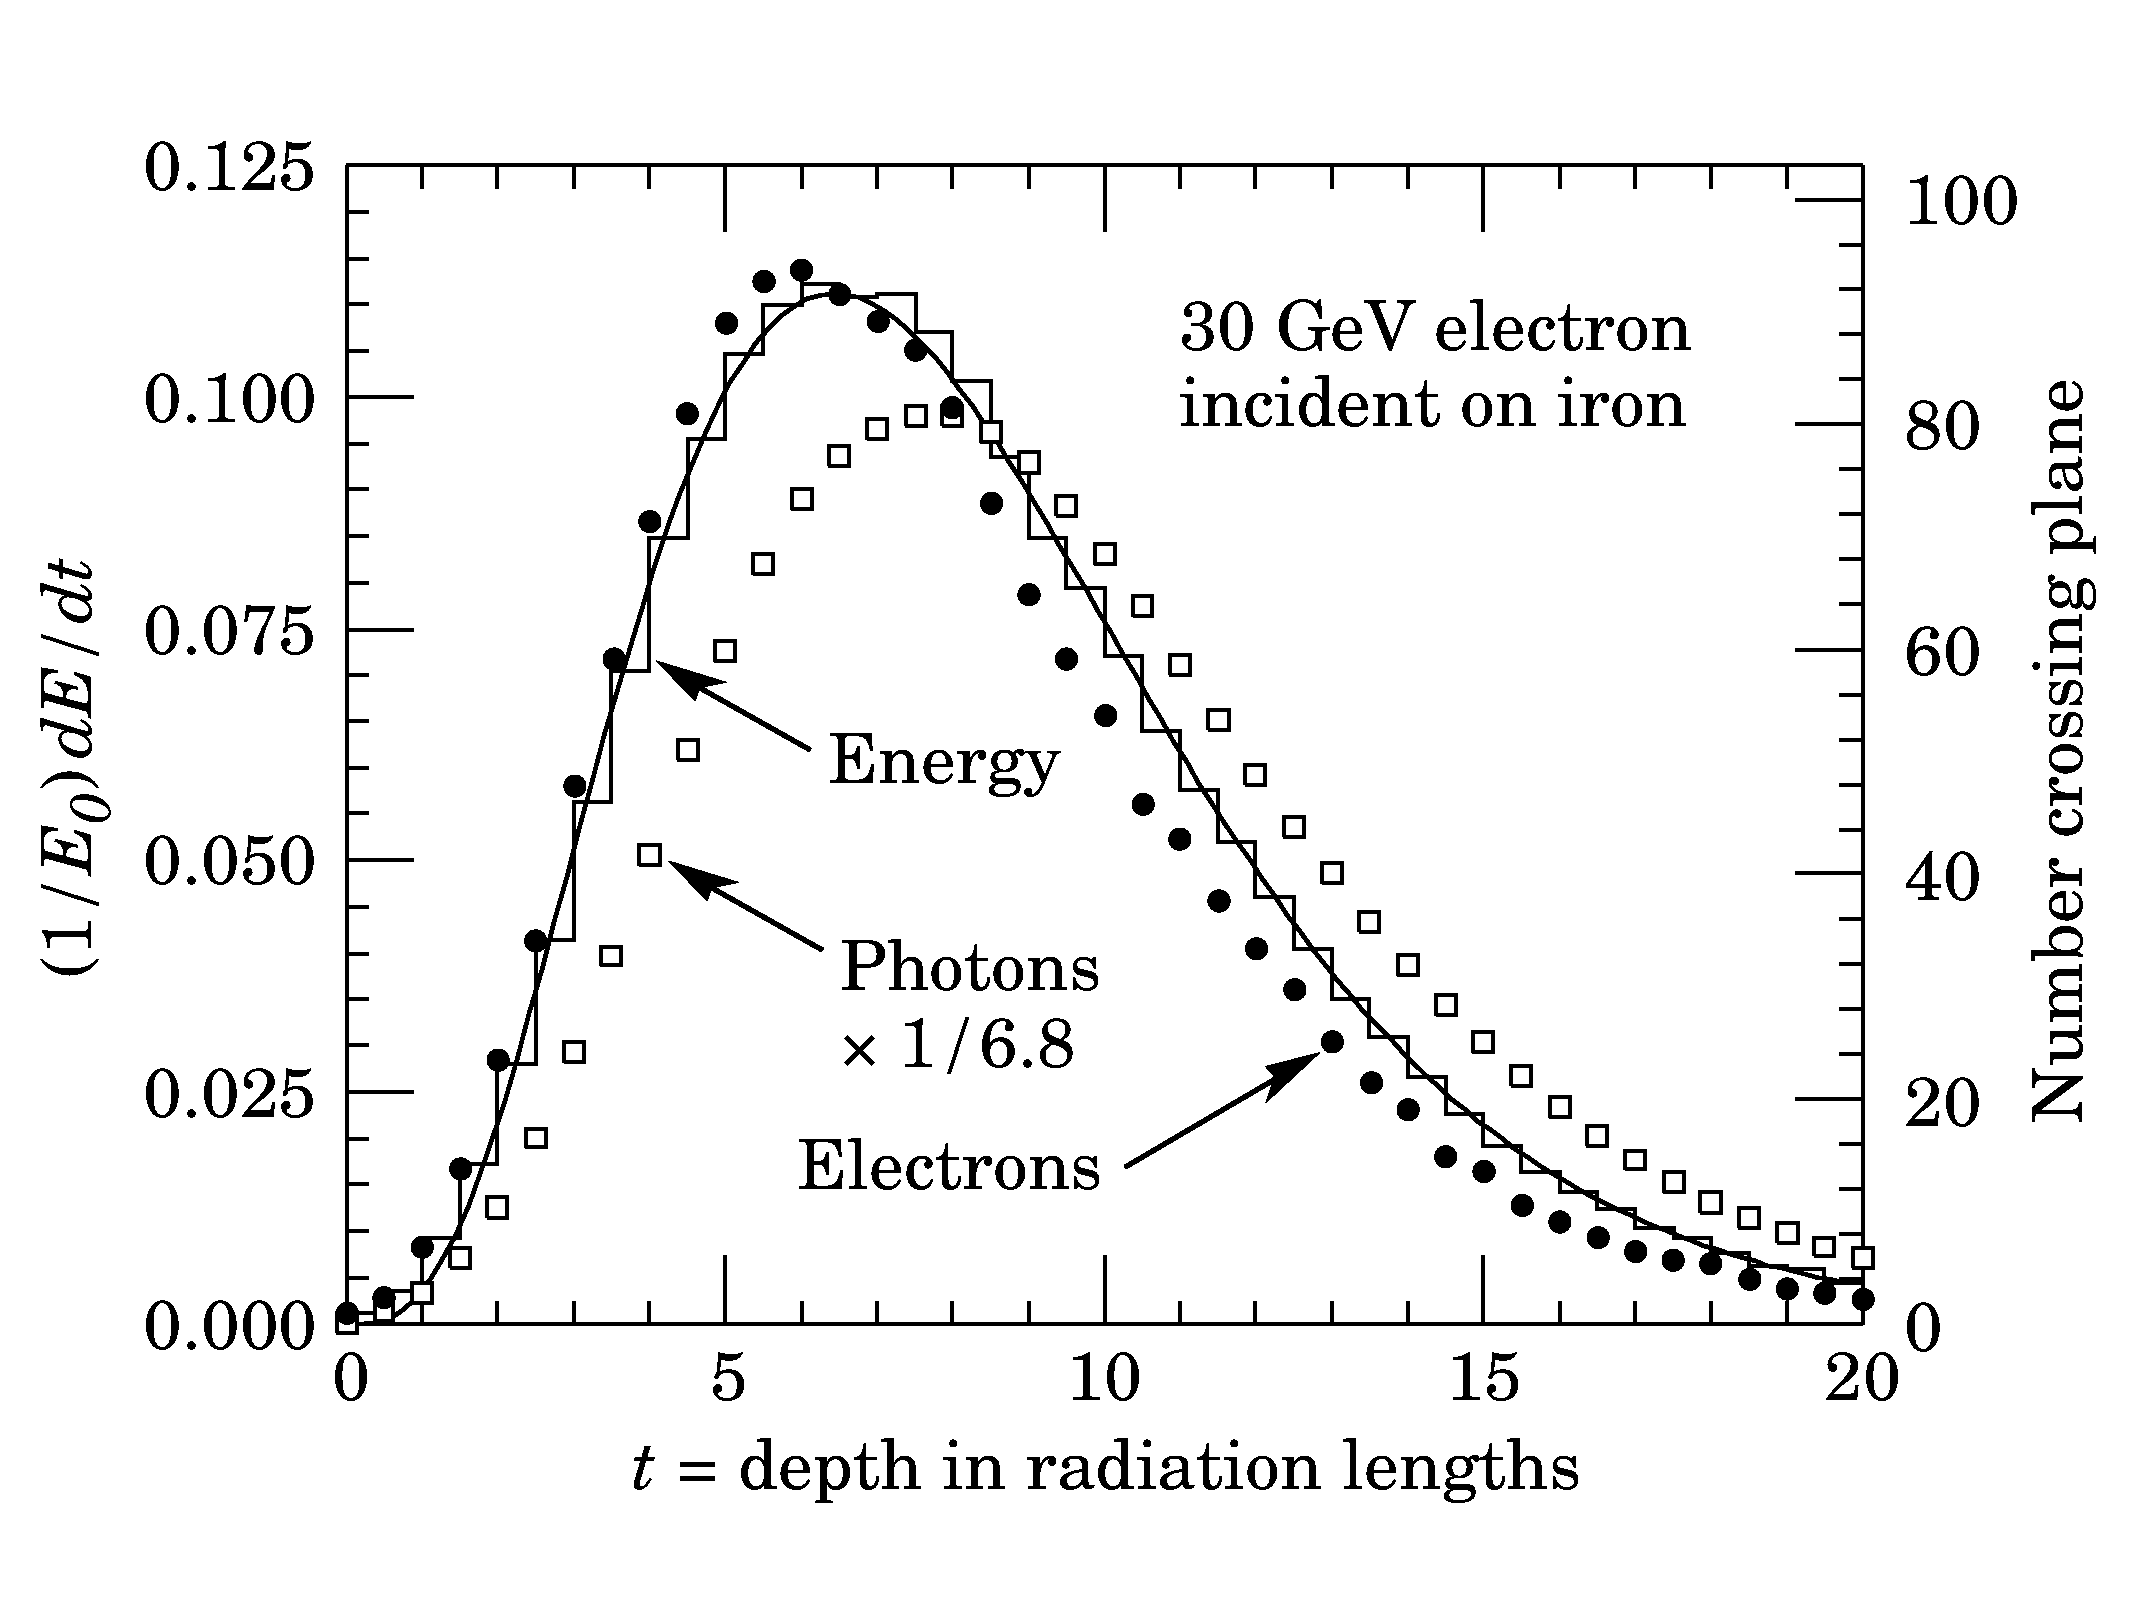
\includegraphics[width=0.85\textwidth]{calorimetry/EGS4_Simulation.pdf}
\caption{Shower profile in the longitudinal direction for
a 30\GeV electron in iron from an EGS4 simulation. The solid line
histrogram shows the fractional energy per radiation length, and the
solid line curve is a fit to the distribution using a gamma
function. The number of electrons (solid circles) and photons
(hollowed squares) with energies larger than 1.5\MeV and crossing
planes at $X_{0}/2$ intervals (scale on the right) is also shown. The
number of photons has been scaled down to have the same area as the
number of electrons distribution.}
\label{fig:showerProfile1}
\end{figure} 
\begin{figure}[h] \centering
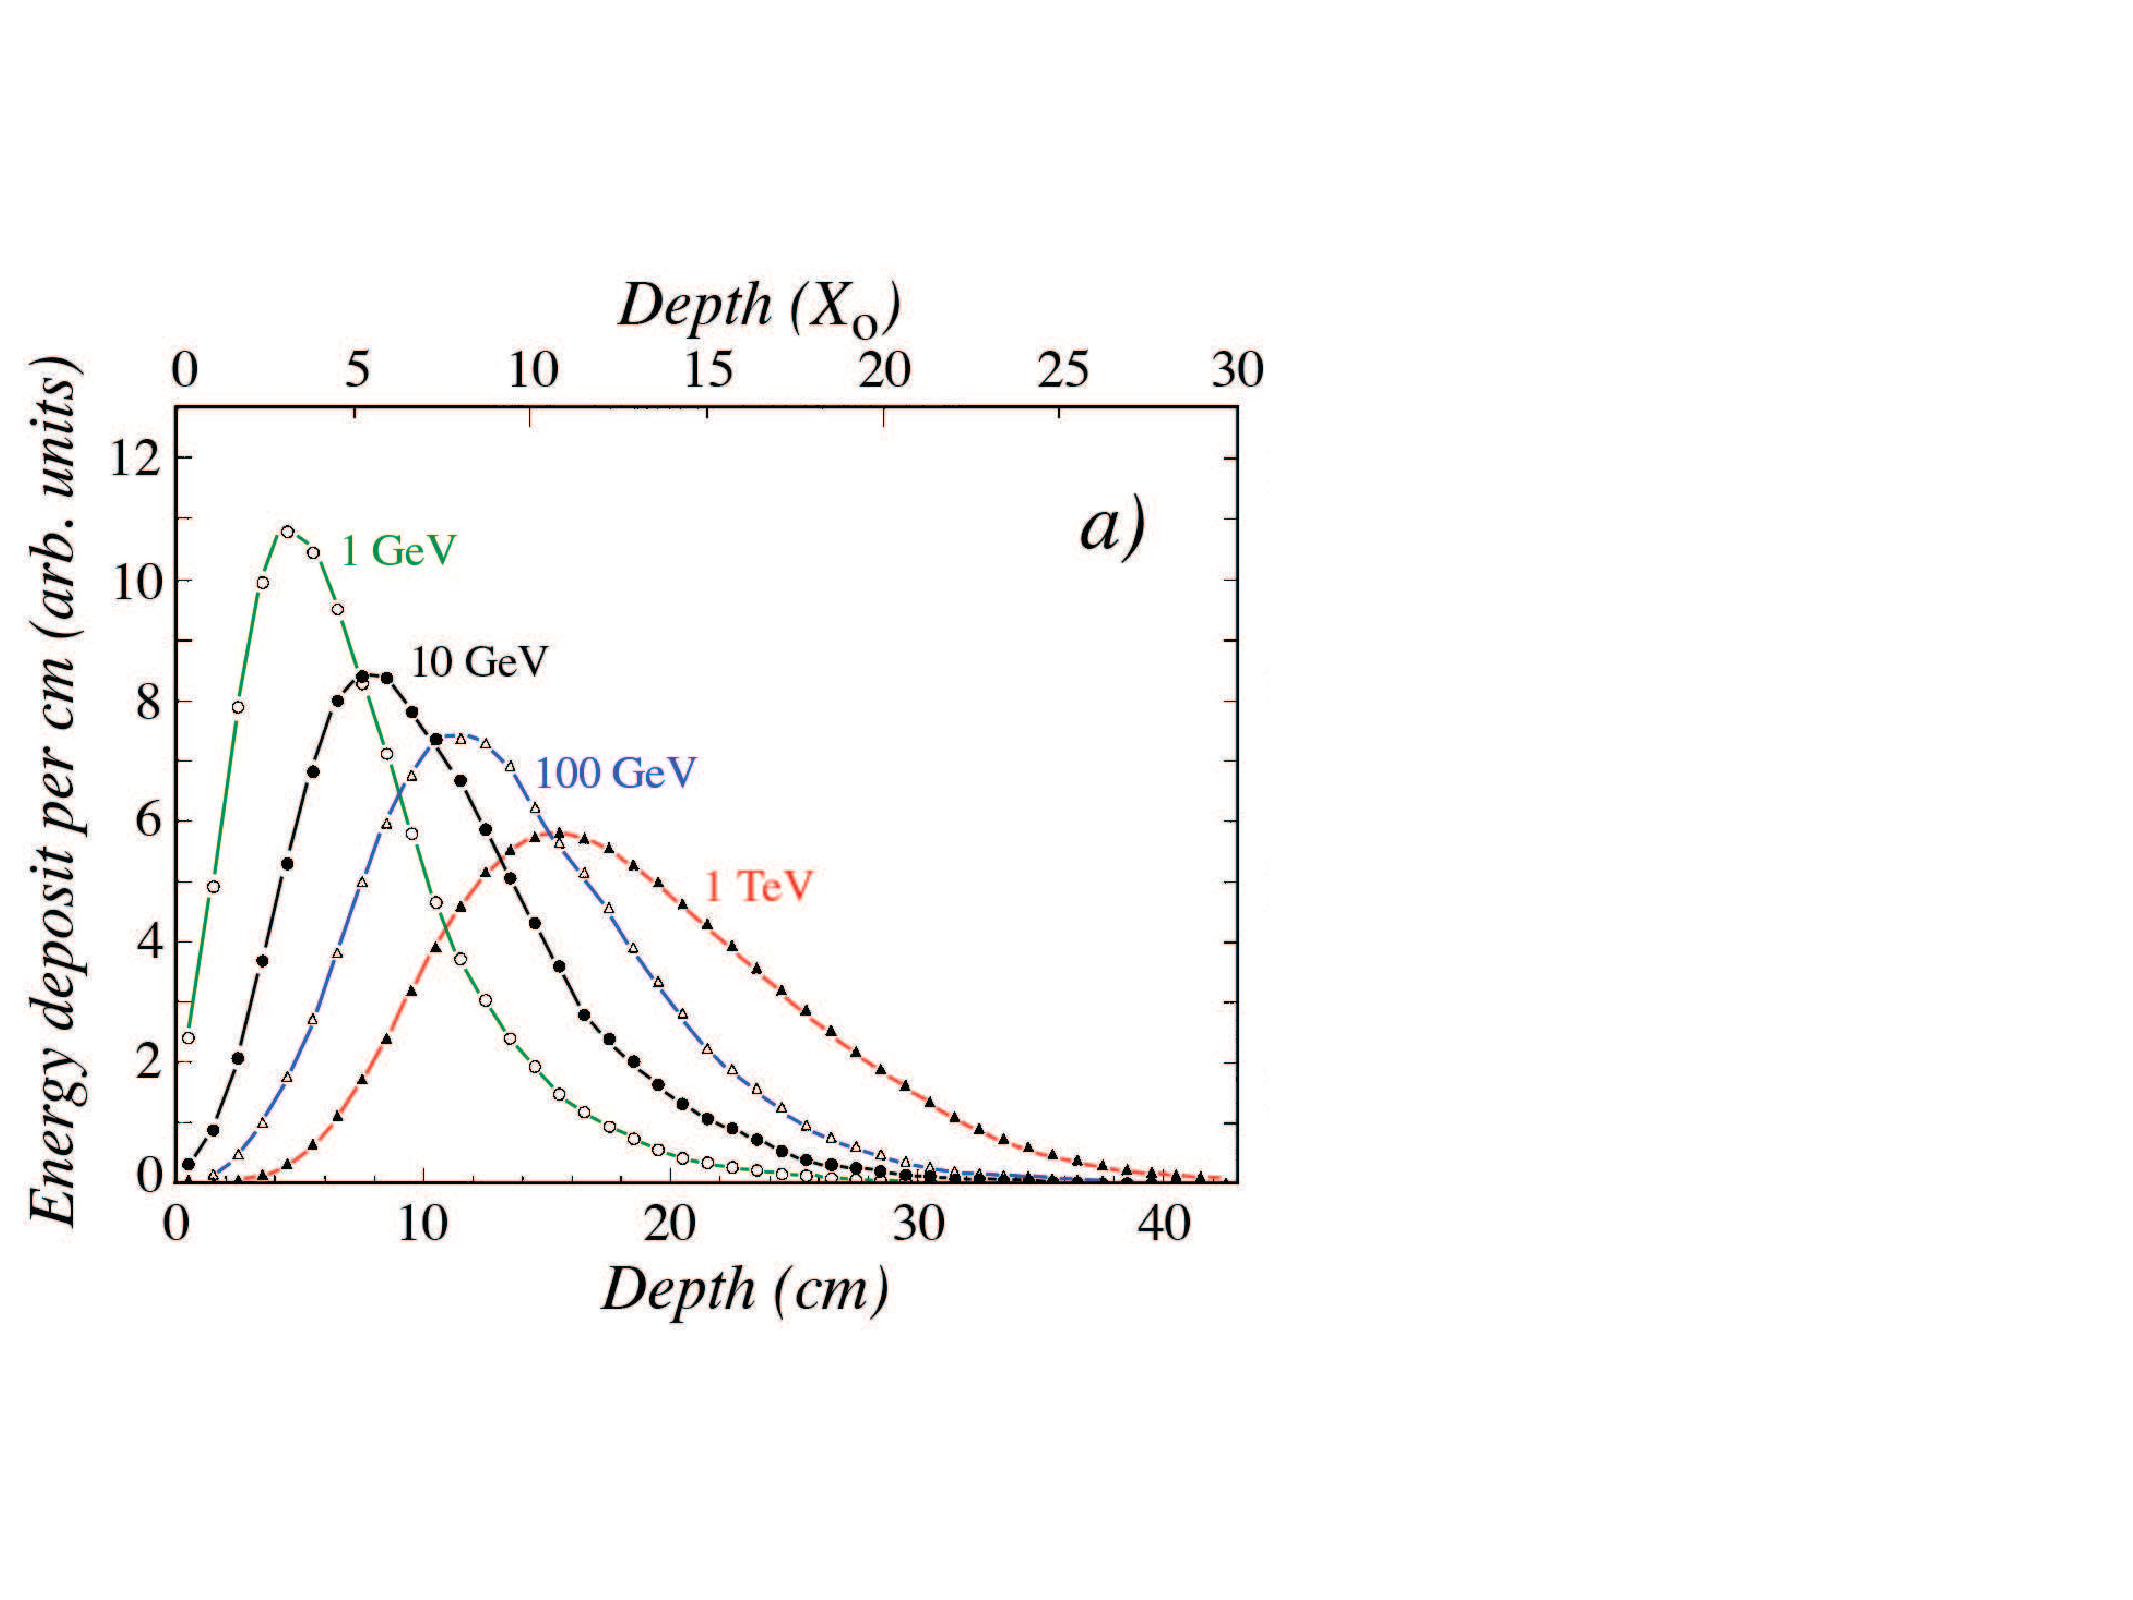
\includegraphics[width=0.85\textwidth]{calorimetry/ShowerProfile_Left.pdf}
\caption{Shower profile in the longitudinal direction for
electrons in copper. The different curves and points represent
different electron energies ranging from 1\GeV-1\TeV.}
\label{fig:showerProfile2}
\end{figure} 

Shower development is described independently of the
calorimeter material by two quantities: the \textbf{radiation length}
($X_{0}$) and the \textbf{Moli\`ere radius} ($R_{M}$). The radiation length is the characteristic amount traversed by high energy
e/$\gamma$s in the longitudinal direction (along the orignal
particle's direction), it is usually measured in $g
\mathrm{cm}^{-2}$. The quantitative definition is (a) the
mean distance over which it  and electron looses 1/$e$ of its initial
energy, and (b) 7/9 of the pair production mean free path for high
energy photons. $X_{0}$ has been tabulated and calculated by Y. S
Tsai~\cite{}, the analytical expression is the following:

\begin{equation}
\frac{1}{X_{0}} = 4\alpha r^{2}_{e}\frac{N_{A}}{A}\left[ Z^{2}\left(
    L_{\mathrm{rad}} - f(Z)\right) + ZL^{'}_{\mathrm{rad}}\right],
\end{equation}

where $\alpha$ is the fine structure constant, $r_{e}$ is the classical
electron radius, $N_{A}$ is Avogadro's number, A is the atomic mass, Z
is the atomic number, $L_{\mathrm{rad}}$ and $L^{'}_{\mathrm{rad}}$
are shown in Table~\ref{tab:Lrad}, and $f(Z)$ is an infinite sum,
nonetheless for chemical elements up to uranium can be expressed to
the 4-decimal place accuracy by

\begin{equation}
f(Z) = (\alpha Z)^{2}\left[ (1+(\alpha Z)^{2})^{2} + 0.2020 - 0.0369
  (\alpha Z)^{2} + 0.0083(\alpha Z)^{4} - 0.0020 (\alpha Z)^{6}\right].
\end{equation}
 
\begin{table}[!ht]
\begin{center}
\caption{Tabulated values for $L_{\mathrm{rad}}$ and
  $L^{'}_{\mathrm{rad}}$ from Y. S Tsai.}
\label{tab:Lrad}
\begin{tabular}{cccc}
\hline
Element & Z & $L_{\mathrm{rad}}$ & $L^{'}_{\mathrm{rad}}$ \\
\hline
H & 1 & 5.31 & 6.144\\
He & 2 & 4.79 & 5.621\\
Li & 3 & 4.74& 5.805\\
Be & 4 & 4.71& 5.924\\
Others & > 4 & ln(184.15$Z^{-1/3}$) & ln(1194$Z^{-2/3}$)\\
\hline
\end{tabular}
\end{center}
\end{table}

The Moli\`ere radius is the characteristic size of the shower in the transverse
direction and defined as the ratio
of the radiation length and the critical energy:
\begin{equation}
R_{M} = X_{0}/E_{c}.
\end{equation} 
The transverse spread of the shower is the result of high
energy $e^{\pm}$ moving away from the shower axis due to multiple scattering, as well as the
isotropic production of low energy electrons a photons. Multiple
scattering dominates the lateral evolution in the early stages while
isotropic production dominates at the later stages of the shower
evolution, after the shower maximum. This two components exhibit a
characteristic exponential decay, see
Figure~\ref{fig:transverseProfile}, where the transverse energy density for
electron showers in copper is shown.
\begin{figure}[h] \centering
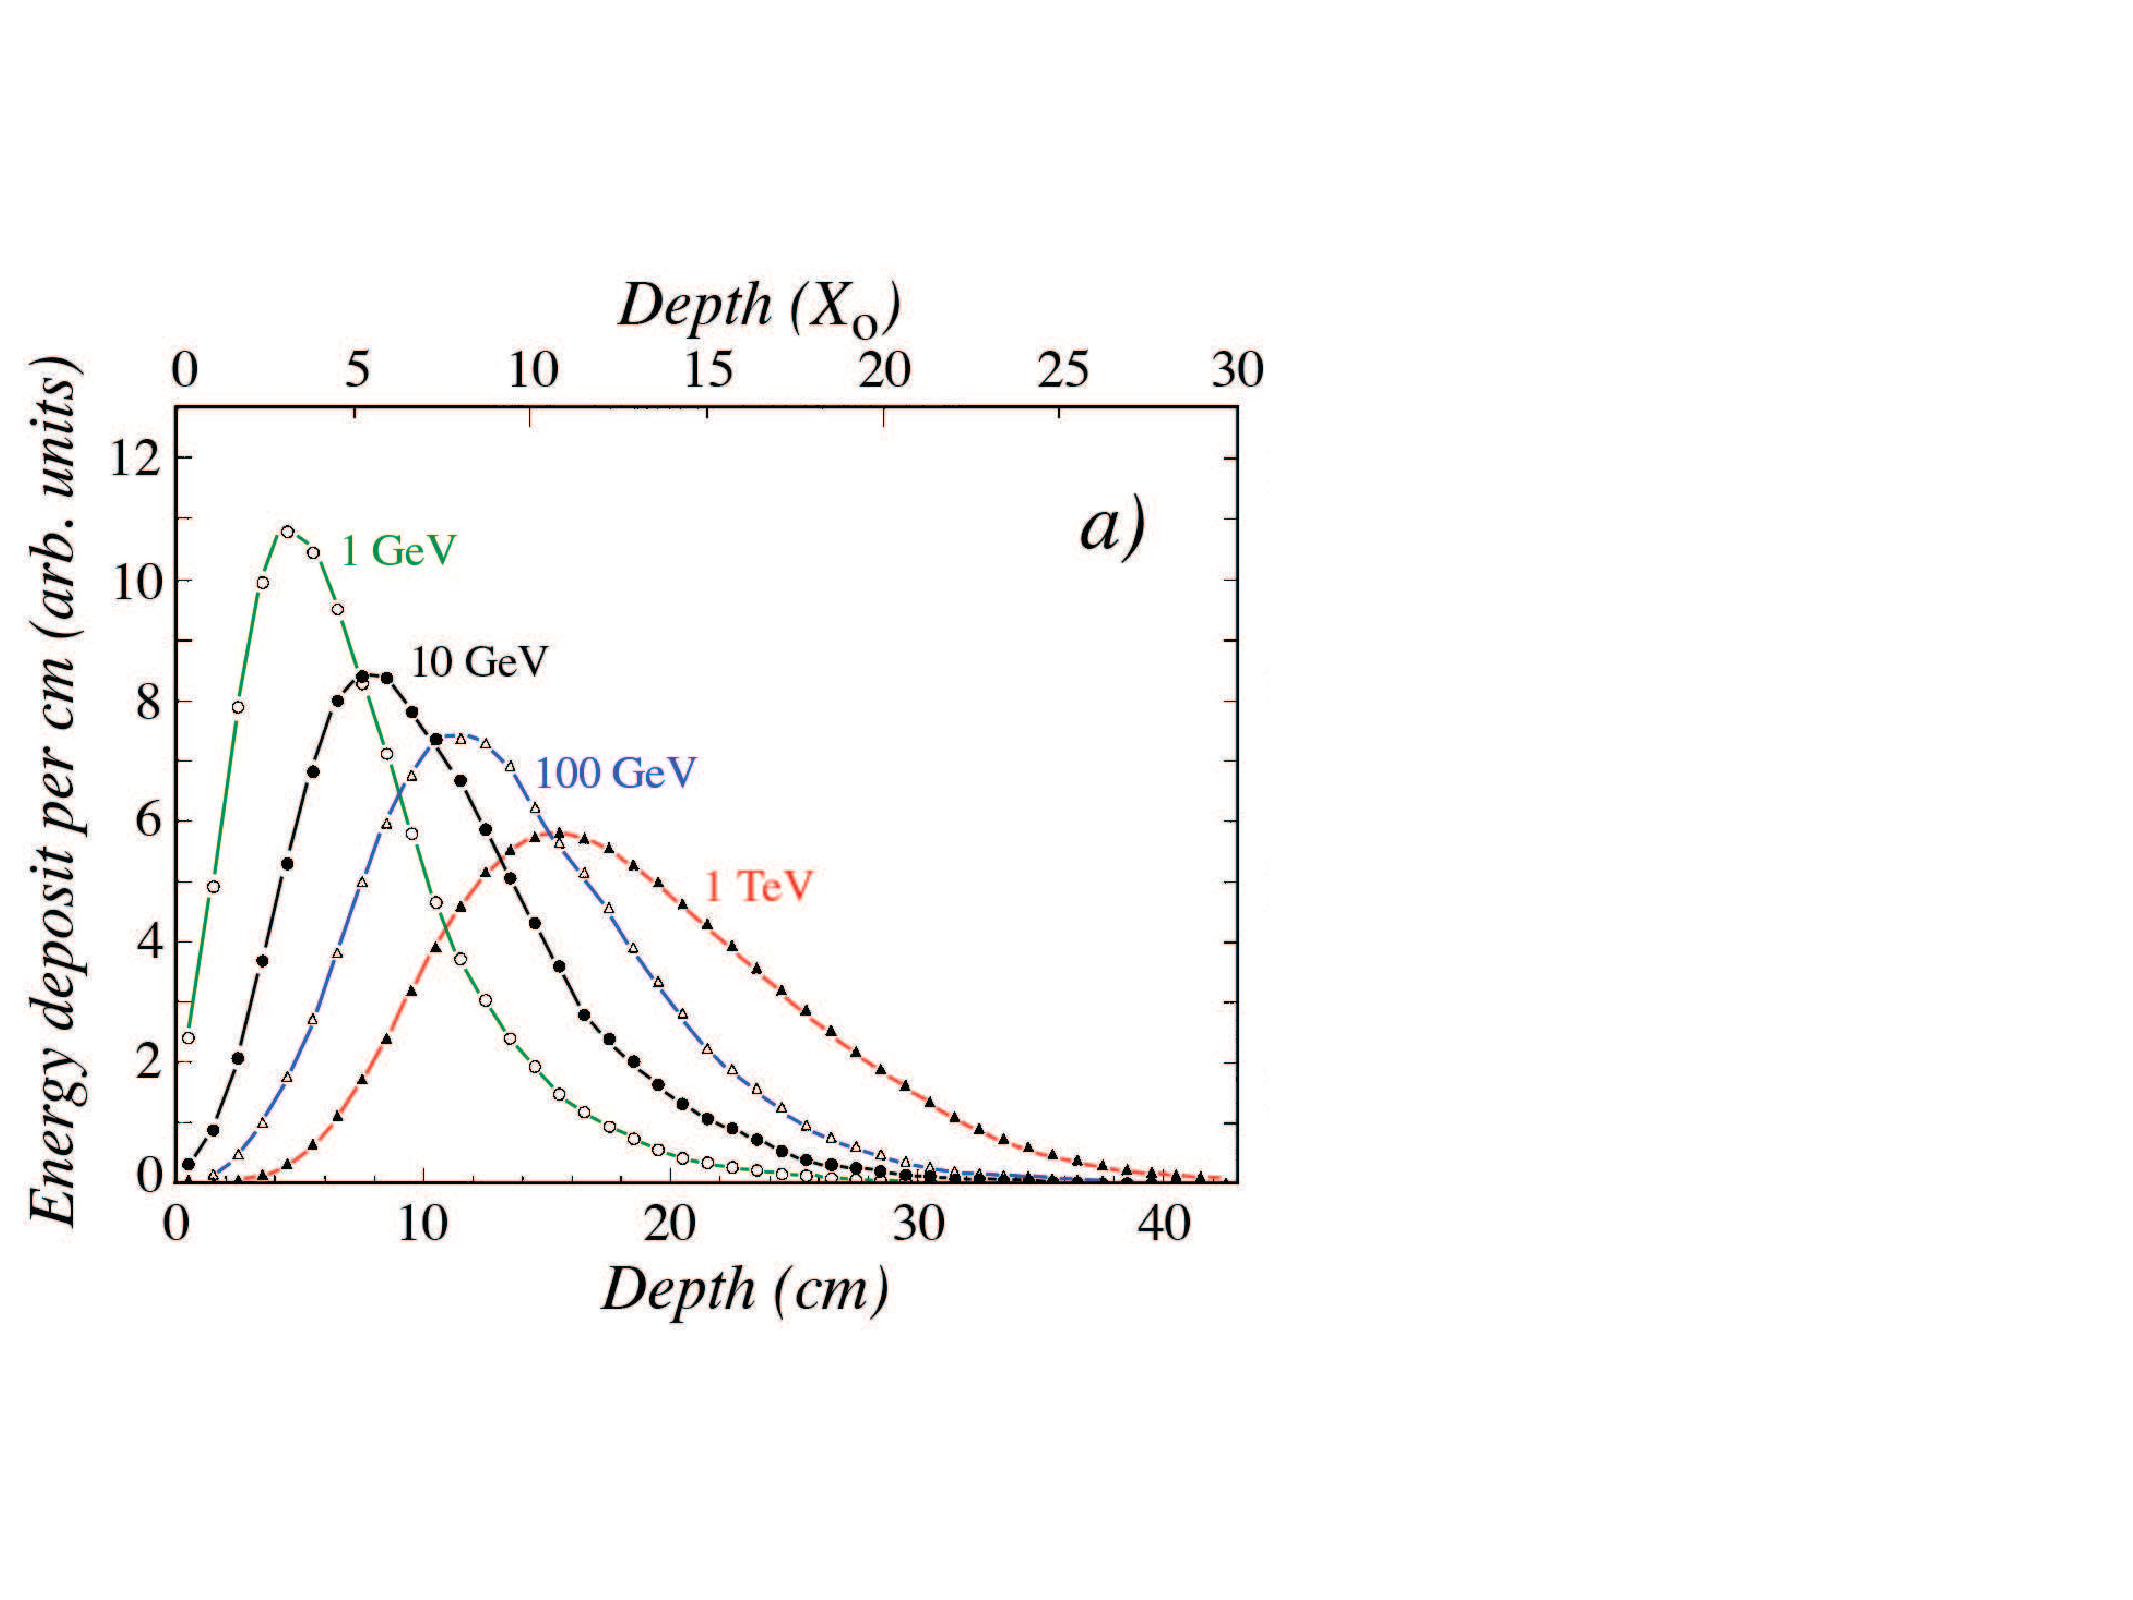
\includegraphics[width=0.85\textwidth]{calorimetry/ShowerProfile_Left.pdf}
\caption{Energy deposited per unit length in the transverse direction for
10\GeV electrons in copper. The shower has been sample in three
different places; at 2$X_{0}$ (red circles), 6$X_{0}$ (black dots),
and 15$X_{0}$ (blue crosses).}
\label{fig:transverseProfile}
\end{figure}

\subsection{Important Calorimeter Quantities}
 xyz

\chapter{LYSO-based Calorimeters}\label{lyso-cal}
This chapter presents studies on measurements of the time of flight using sampling calorimeters 
based on LYSO crystals. 

\section{Introduction}
Due to its very high light yield 
($\sim 30$K photons/MeV)~\cite{LYSOProperties}, and radiation 
tolerance~\cite{5402126, 4291695, 5402125, Dissertori:2013rma}, LYSO
is the active element of one of the options considered for the upgrade of the
Compact Muon Solenoid (CMS) detector for the HL-LHC~\cite{Contardo:1605208}. 

In Figure~\ref{fig:ScintillatorTiming} presents a simplified illustration of
the major time scales associated to the timing measurement using a monolithic
crystal calorimeter. Upon entering the crystal the photon or electron travels
at the speed of light, interacts, and begins to shower, producing scintillation light in the crystal. 
The time between the entry of the photon into the crystal and the first interaction is denoted by
$t_I$ and for high energy impinging particles it is the shower development time. 
The time associated with the conversion of the incident photon to
scintillation light is denoted by $t_S$. The scintillation light travels from
the point of interaction to the photodetector at the velocity $c/\hat{n}$, where
$\hat{n}$ is the effective index of refraction of the crystal~\cite{Moses}. The
time associated with the propagation of the scintillation light to the photodetector 
is denoted by $t_P$. Once the scintillation light reaches the photodetector, the  photons 
are converted into an electrical signal. The time associated with this process is known as the
photodetector signal transit time, $t_T$. Finally, the data acquisition (DAQ)
system has a characteristic time constant $t_D$. Each of these time intervals will fluctuate or 
jitter on an event-by-event basis, contributing to the time resolution.
\begin{figure}[h] \centering
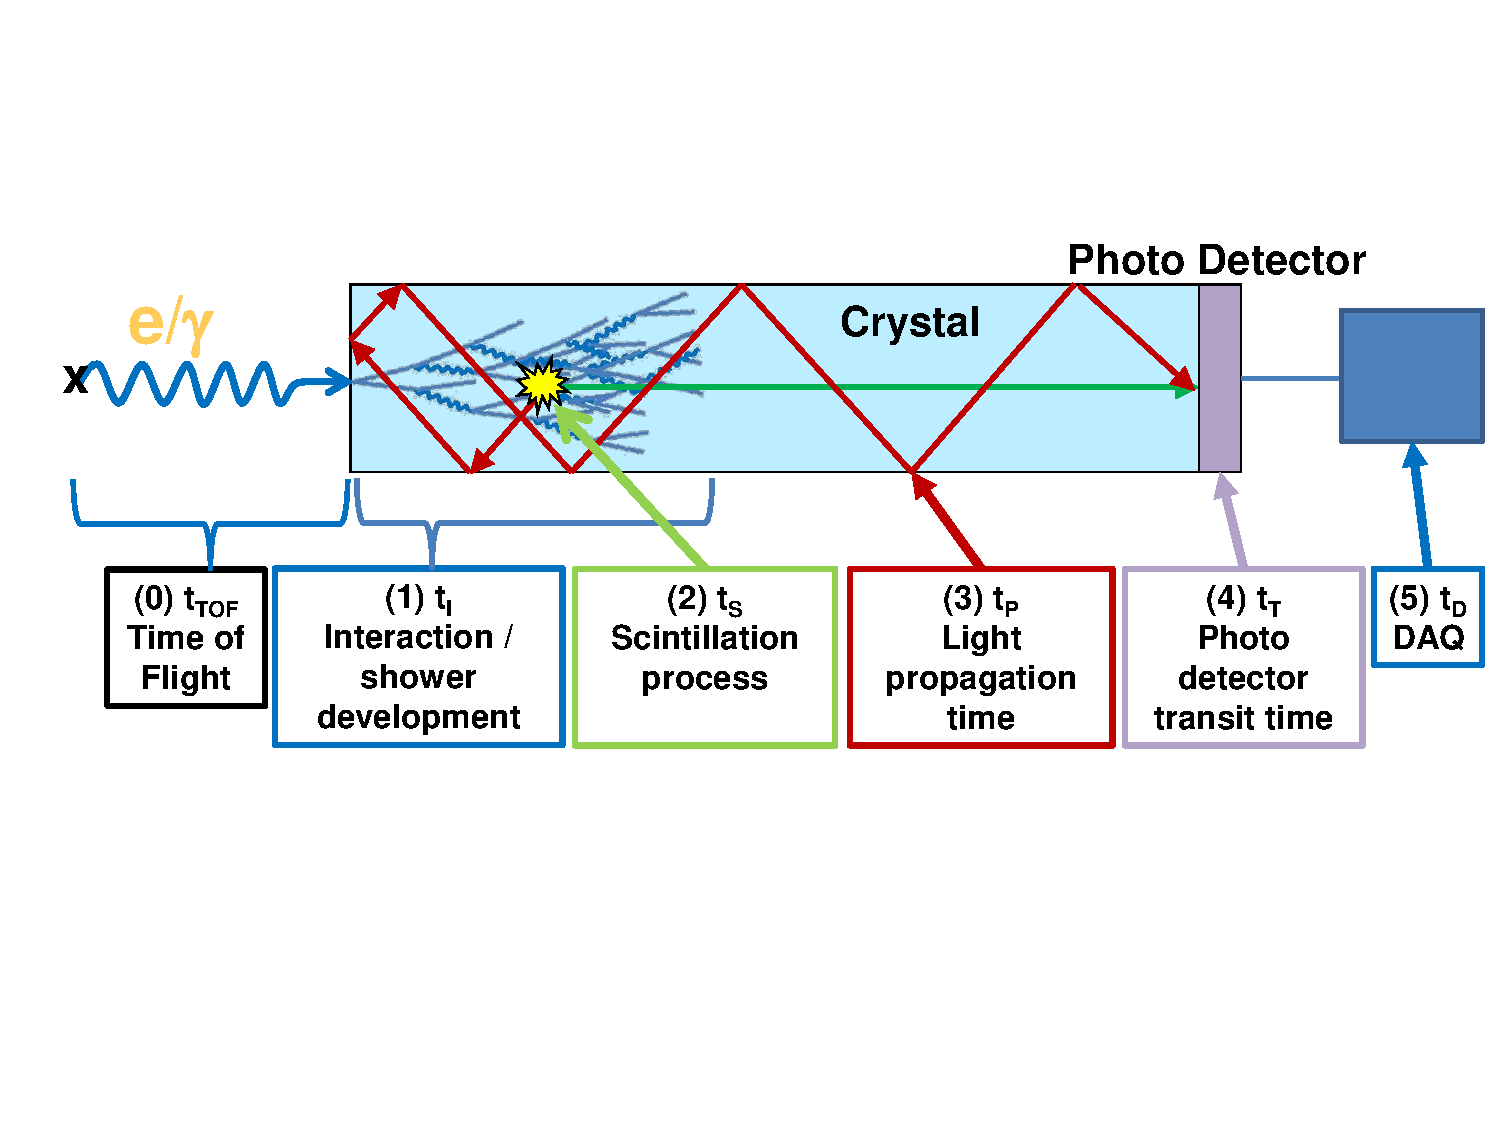
\includegraphics[width=0.85\textwidth]{figs/ScintillatorTiming_v4}
\caption{\small Timing measurement schematic breakdown using a monolithic, large scintillating crystal. 
The incident particle impinges on the crystal face from the left. The characteristic time intervals  are discussed 
in the text.}
\label{fig:ScintillatorTiming}
\end{figure}
Previous studies~\cite{MCPFastCaloNIMA}, measured the time resolution at different
absorber thickness for electron beams with energies varying from $12$ to
$32$~GeV, and showed that the time of arrival of the front of an electromagnetic
shower can be determined with a precision better than $20$~ps. The electronic
time resolution of the DAQ system was measured to be about $6$~ps. Using
the same techniques, the time resolution of the MCP-PMT photodetectors 
used in the studies presented in this paper have been measured to be between $11$~ps and $14$~ps, depending 
on the exact device.

To characterize the time resolution of an inorganic crystal scintillator calorimeter we
study the contributions due to fluctuations in the shower development, scintillation process, 
and light propagation to the photodetector.  We take advantage of the very large number of 
scintillation photons in a LYSO crystal which result in modest fluctuations associated with the 
creation and transit of each particular scintillation photon for a LYSO-based detector. 

\section{Experimental Setup}
A schematic diagram of a typical time of flight measurement setup is shown in 
Figure~\ref{fig:TypicalSchematicDiagram}. All measurements involve a fast photodetector,  
typically a micro-channel-plate photo-multiplier-tube 
(MCP-PMT), which  measures the reference timestamp ($t_{0}$), and a photodetector further 
downstream that detects the signal associated with the electromagnetic shower and provides 
a simultaneous energy and time ($t_{1}$) measurement. 

\begin{figure}[ht!] \centering
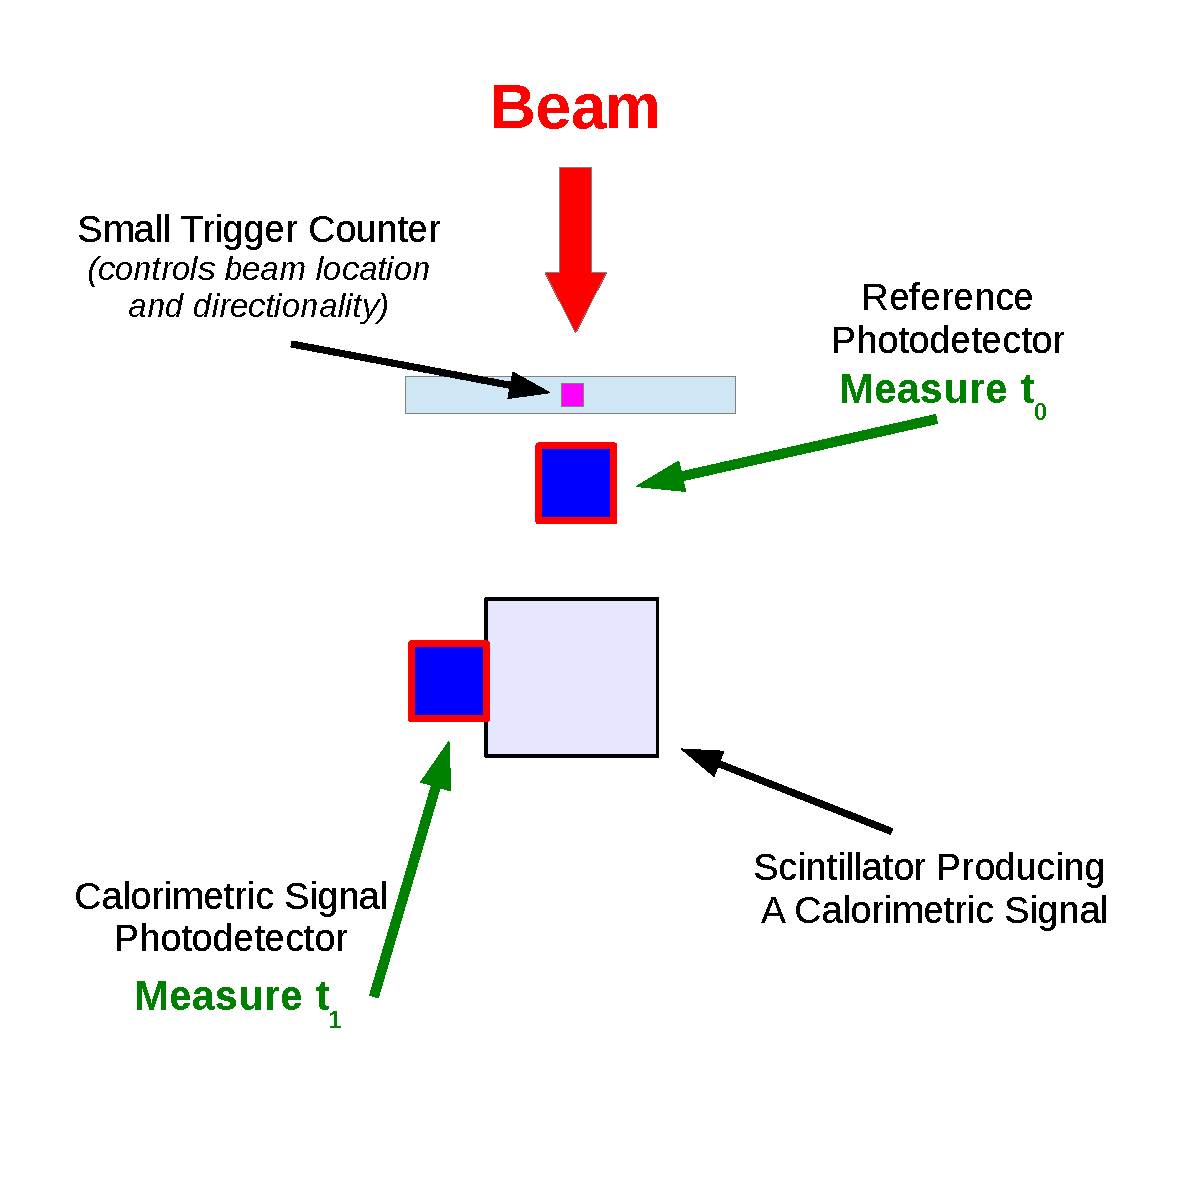
\includegraphics[width=0.45\textwidth]{figs/TypicalSchematicDiagram} 
\caption{\small The basic schematic diagram of the experimental setup for
a typical time of flight measurement is shown to illustrate the
basic detector elements. One photodetector is used as a time reference and the second 
measures energy and time simultaneously.} 
\label{fig:TypicalSchematicDiagram}
\end{figure}

In these studies, two types of MCP-PMT photodetectors are used, one produced by Hamamatsu 
(model R3809-52)~\cite{HamamatsuMCP3809}, and one produced by Photek (model
PMT240)~\cite{Photek240}. A DRS4  waveform digitizer V4 evaluation
board ~\cite{DRS4} was used as the primary DAQ system, connected to a laptop via
USB interface.  The DRS chip contains a switched capacitor array (SCA) with 1024 cells, 
capable of digitizing eight analog signals with high speed (5 GSPS) and high 
accuracy (11.5 bit SNR). All experimental beam studies were performed at the Fermilab Test
Beam Facility (FTBF), which provided proton beams from the Fermilab Main
Injector accelerator at $120$ GeV, and secondary electron beams of energies
ranging from $4$ to $32$~GeV. All detector elements were placed inside of a dark box
lined with copper foil, providing RF shielding. A $2$x$2$~$\mathrm{mm}^{2}$
scintillator was placed inside the box at the upstream extremity and used to
trigger the DAQ readout, providing a strict constraint on the
location and directionality of the beam particles used in the time of flight
studies. A differential Cherenkov counter (not shown in the schematic)  provided by the FTBF
facility and located upstream of our experimental hall,  was used for electron
identification. 

\section{Event Selection and Data Analysis}

The primary target is to reconstruct the time of flight of beam particles between
different detector elements. Different time reconstruction algorithms are used
for different detector elements, and all involve the assignment of a timestamp
using specific features of each corresponding signal pulse. The signal pulse for
the reference time detector is very sharp and symmetric around its maximum
amplitude, as shown in Figure~\ref{fig:PulseShapes}. Hence for the reference
detector we determine the time position of the pulse peak by fit a Gaussian
function to the peak of the pulse, using three sampling points before the pulse
maximum and four sampling points after. The fitted mean parameter of the
Gaussian function is assigned as the timestamp $t_{0}$. The signal pulse for the
downstream time measurement is the result of scintillation light, and exhibits a
fast rising edge and a significantly slower decay. Therefore, we assign the
timestamp $t_{1}$ using a constant fraction of the rising edge. A linear
function is fit to the sampling points between $10\%$ and $60\%$ of the pulse
maximum and the timestamp is assigned as the time at which the fitted linear
function rises to $20\%$ of the pulse maximum. Examples of fits performed to
assign a time stamp from each pulse are shown in Figure~\ref{fig:PulseFits}. The
impact from the choice of the functional forms is studied by using a set of
alternative functions in the fits, and choosing the one that results in the best
time resolution. Among the functions that we tested, the difference between the
best and worst performing functions was about 8~psec.

\begin{figure}[h] \centering
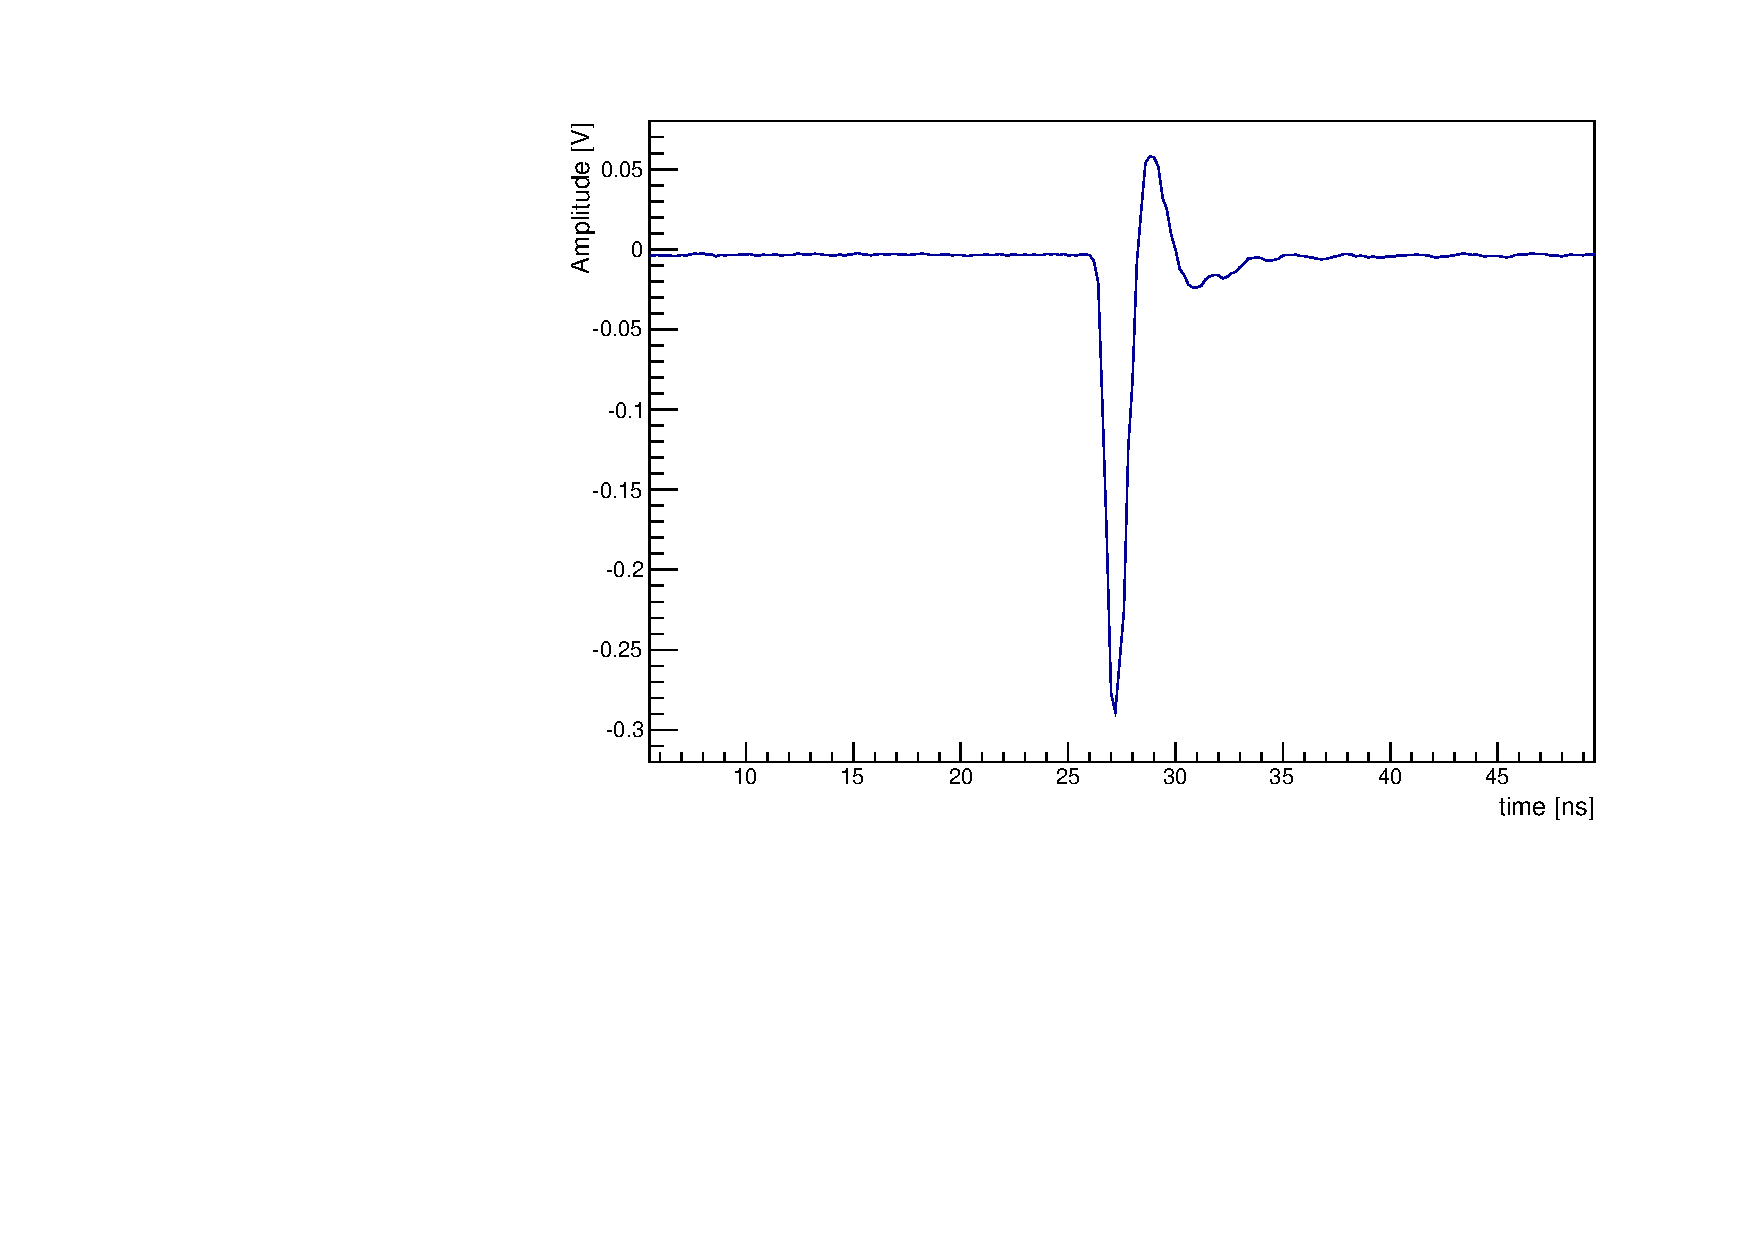
\includegraphics[width=0.45\textwidth]{figs/RefPulse} 
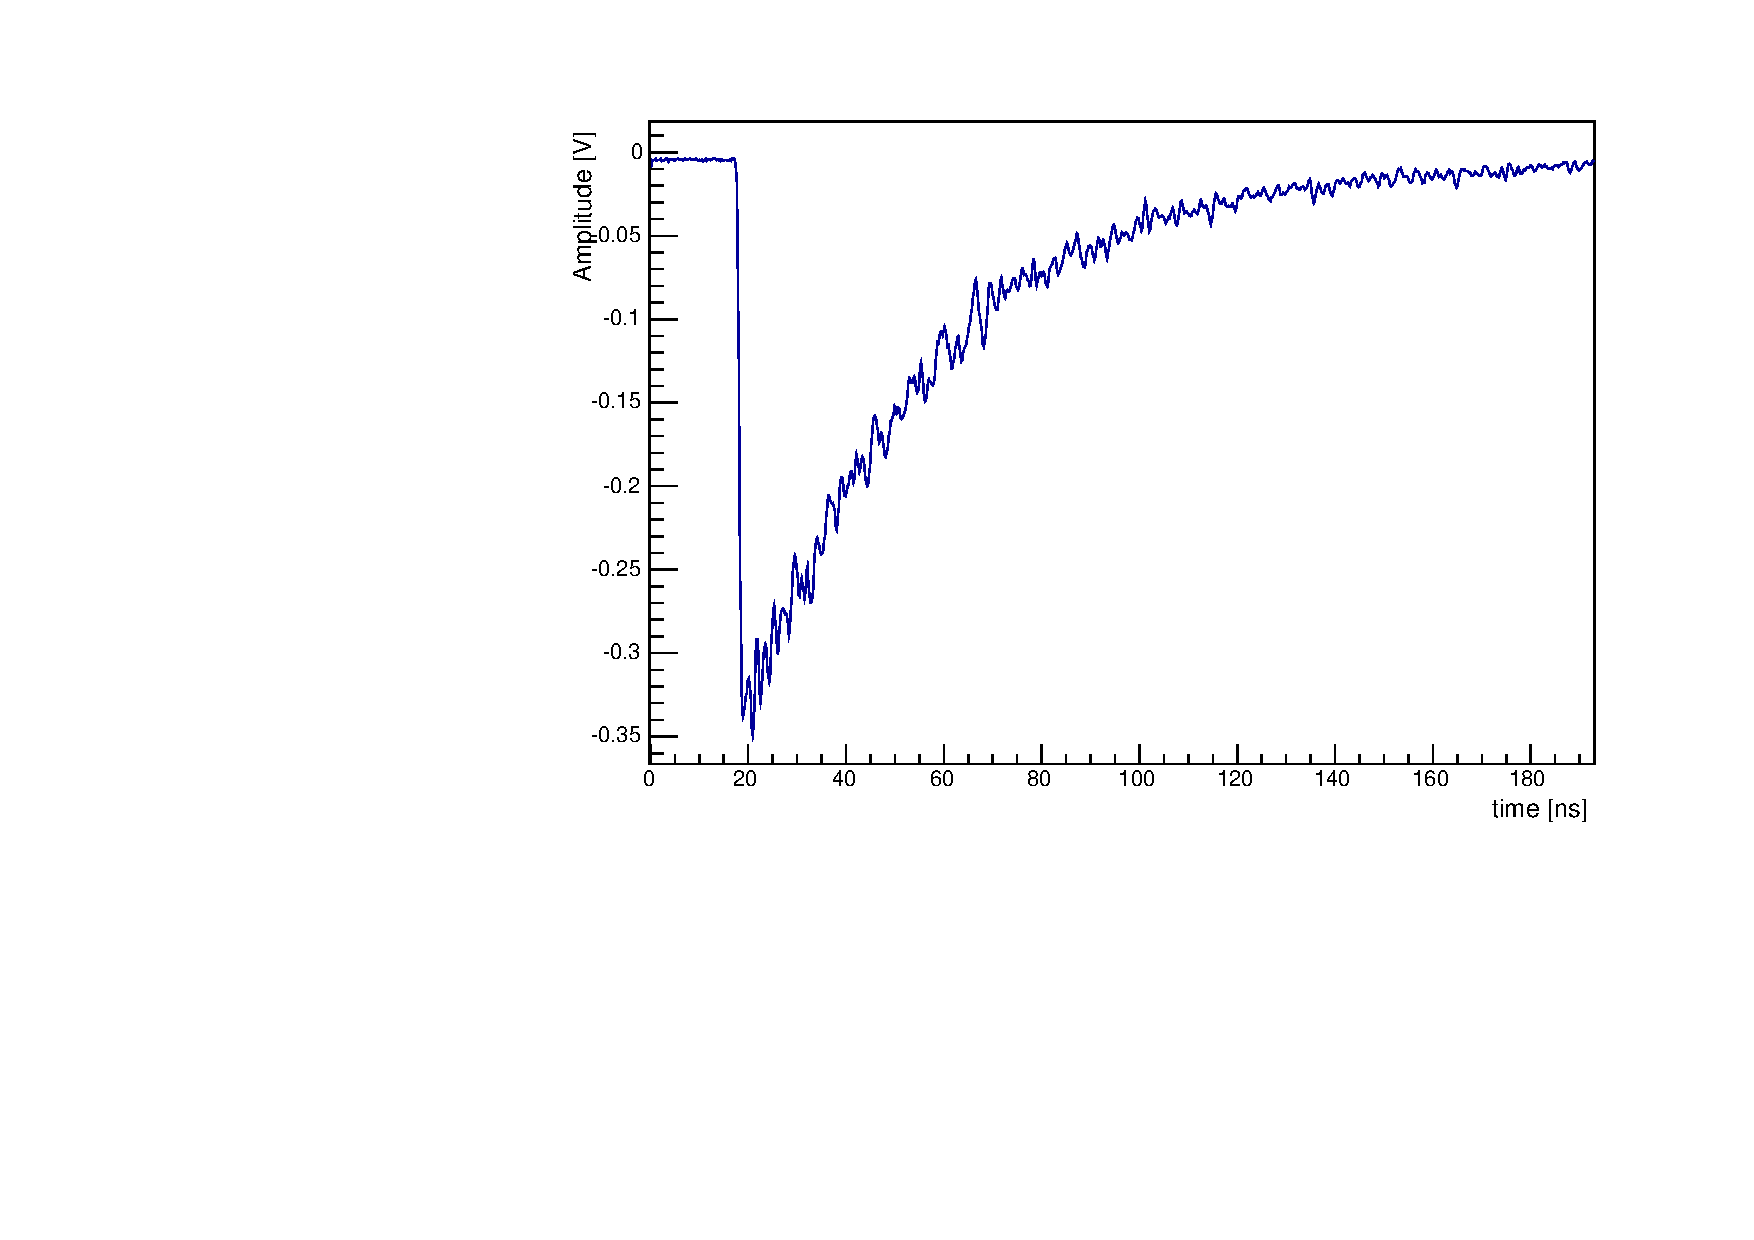
\includegraphics[width=0.45\textwidth]{figs/run064_event506} 
\caption{\small Sample pulses as digitized by the DRS4 board. 
On the left a pulse is shown from the reference Hamamatsu R3809 MCP-PMT, 
and on the right is a pulse from the Hamamatsu R3809 MCP-PMT
optically coupled to a (1.7~cm)$^{3}$ LYSO crystal cube
recorded using  8 GeV electron beam.} 
\label{fig:PulseShapes}
\end{figure}

Event selection and pulse cleaning procedures are used to eliminate abnormal
pulses in the readout, as described in~\cite{MCPFastCaloNIMA}. Large signals
above 500 mV are rejected because they saturate the DRS4 inputs. Only pulses
with amplitude larger than 20 mV are used for time of flight measurements, in
order to reduce the impact of noise from the DRS waveform digitizer DAQ system.
Events containing more than one pulse within the $200$~ns readout window are not
used. Attenuators were used to extend the dynamic range of the DRS4
waveform digitizer in cases when a large fraction of signal pulses are saturated.

\begin{figure}[h] \centering
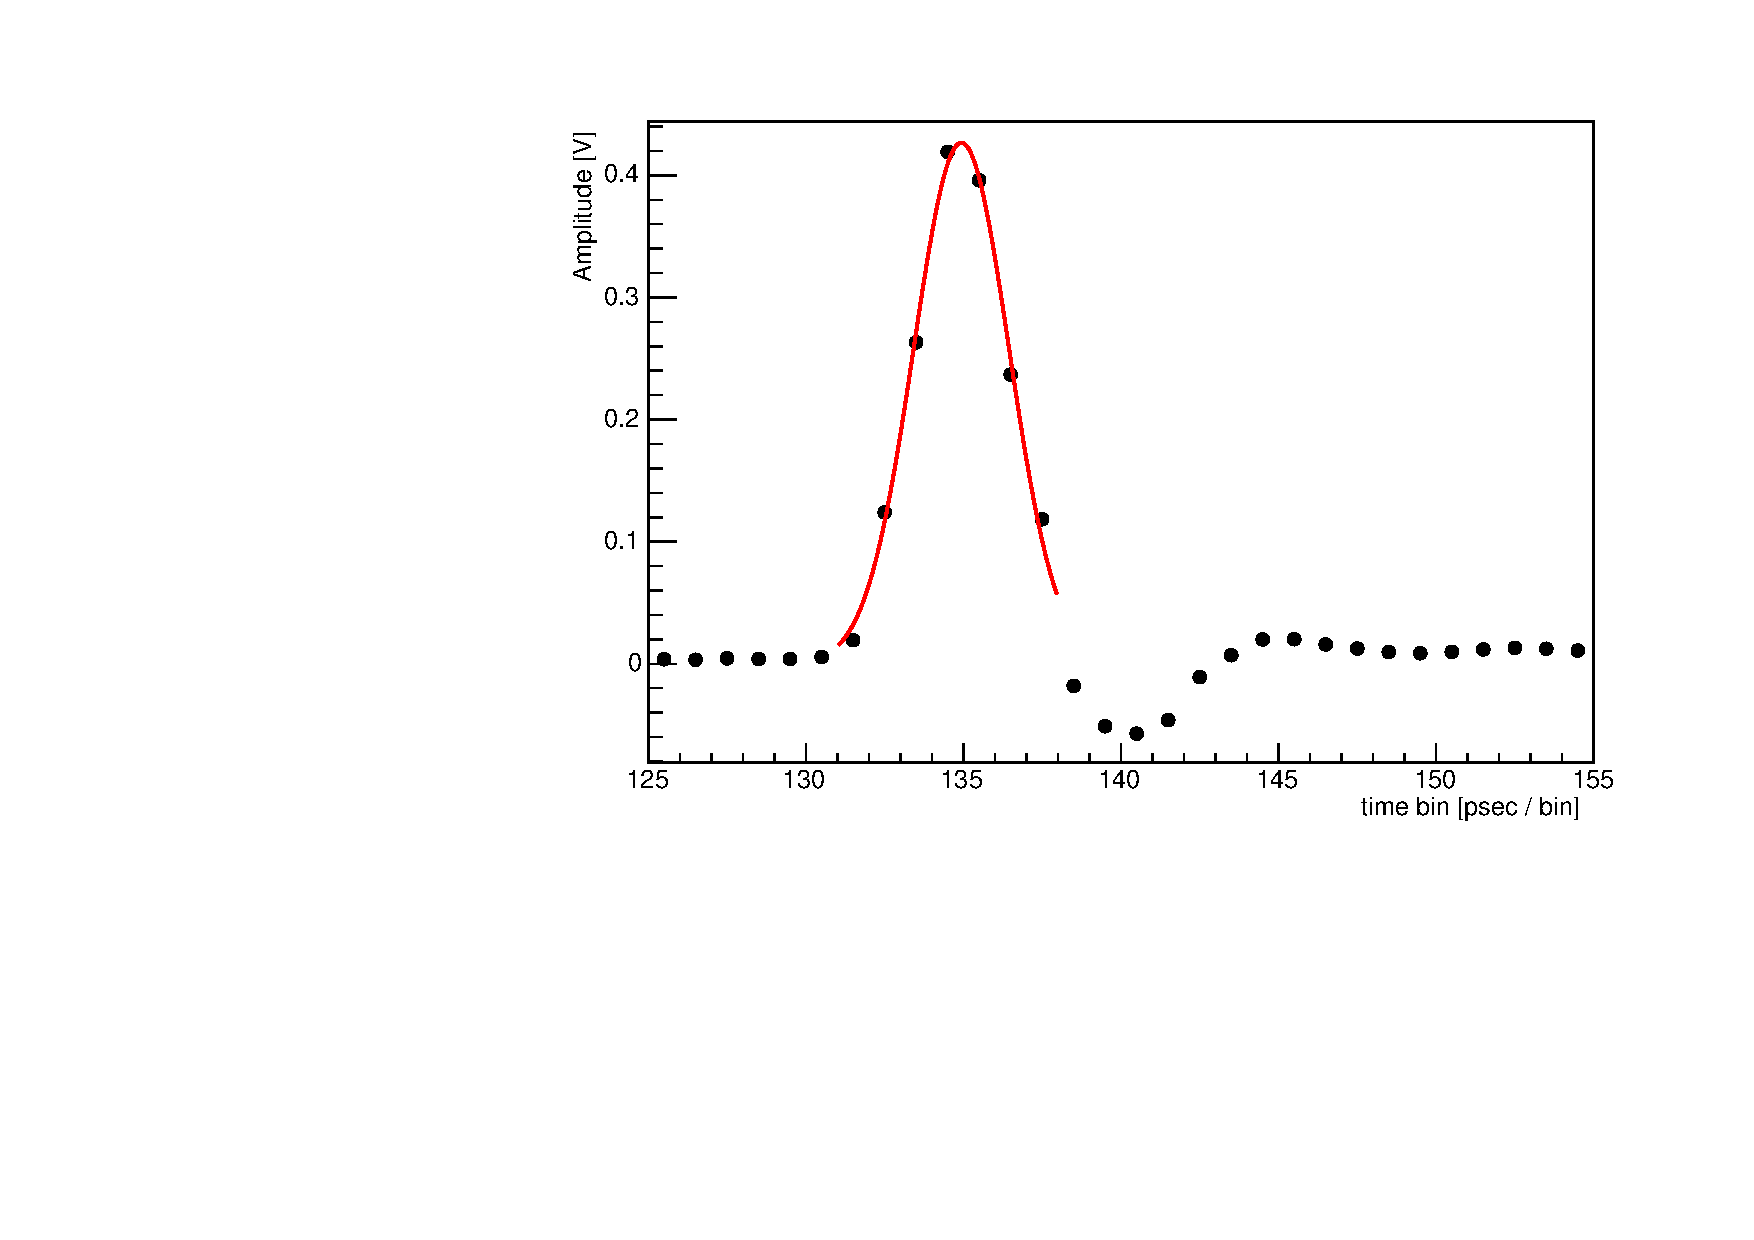
\includegraphics[width=0.45\textwidth]{figs/Reference_Pulse_GausFit_057_ev322.pdf} 
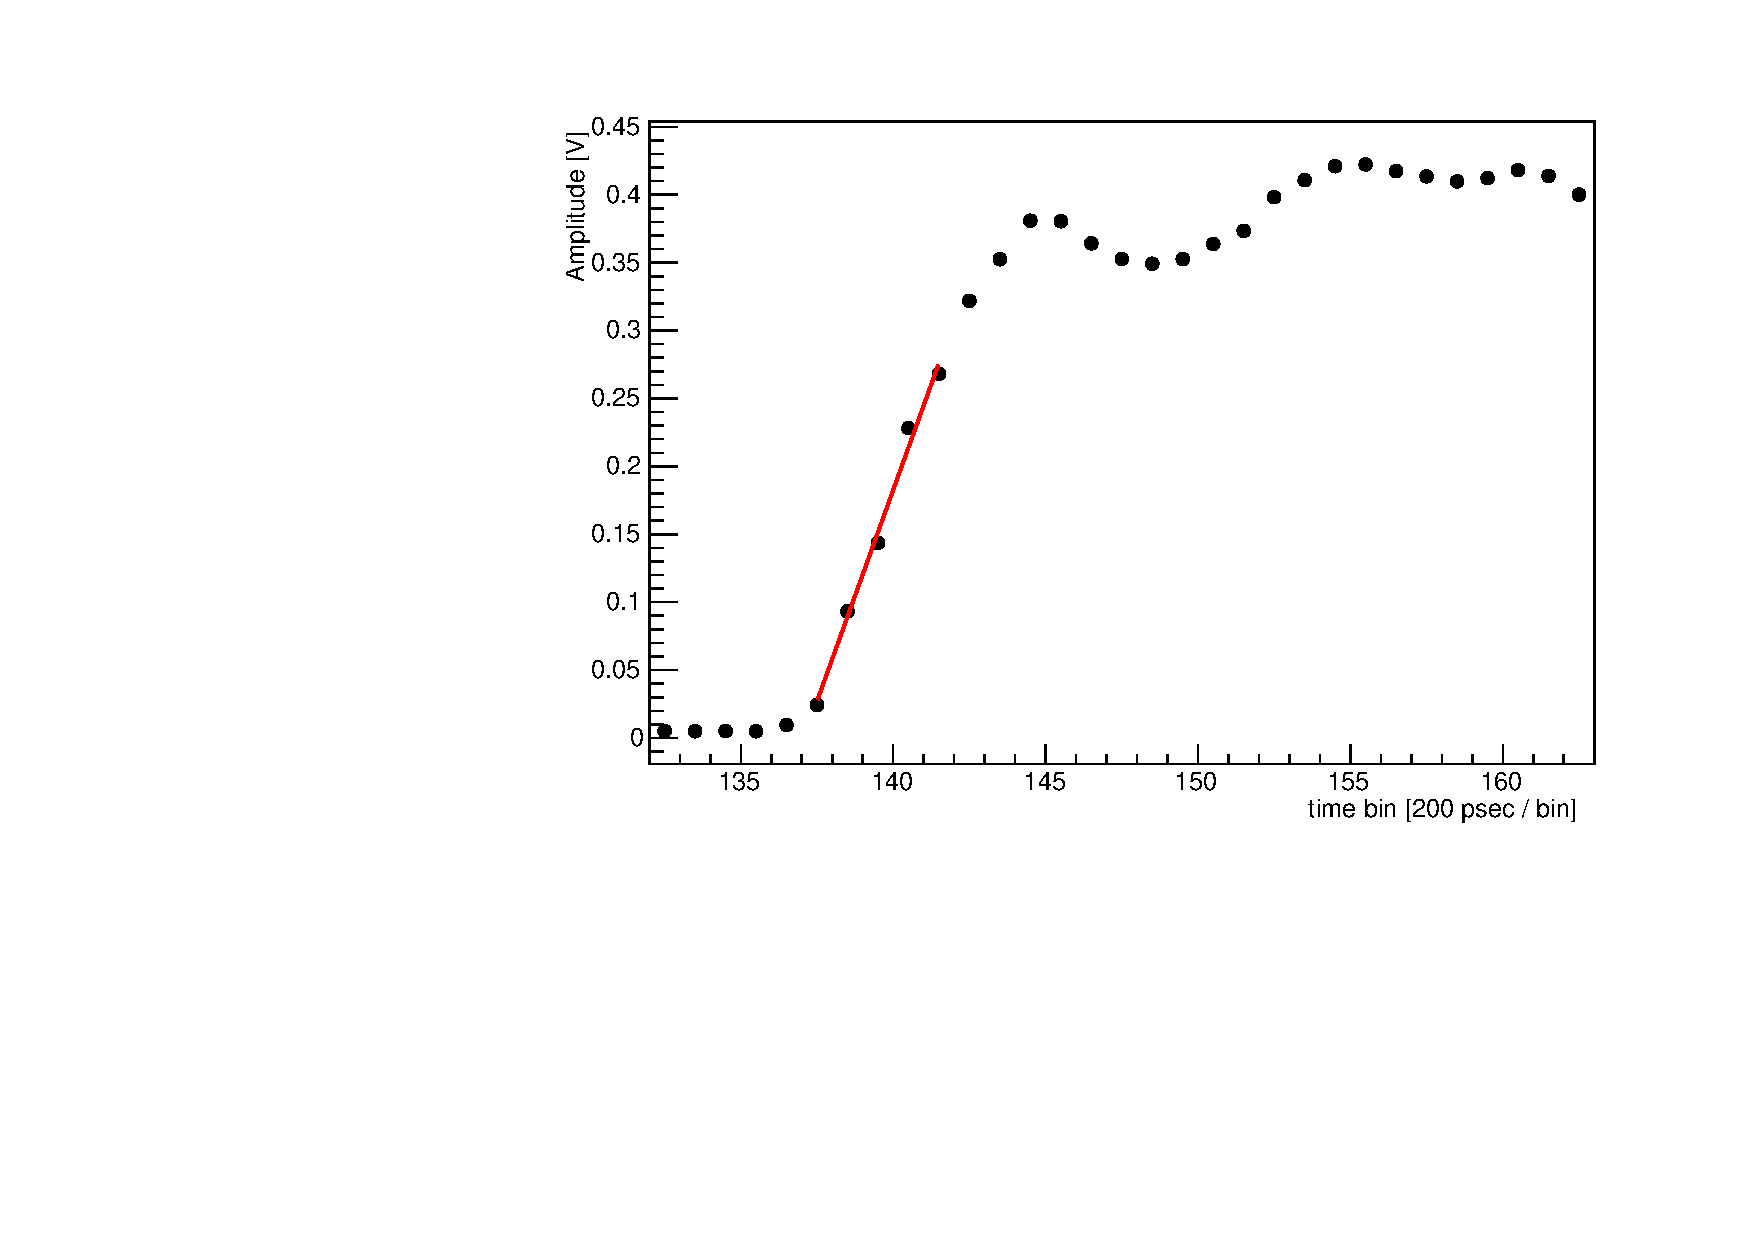
\includegraphics[width=0.45\textwidth]{figs/LYSOCube_Pulse_RisingEdgeFit_057_ev313.pdf} 
\caption{\small Sample fits used to assign timestamps to digitized MCP-PMT pulses. 
On the left is a pulse from the reference Hamamatsu R3809 MCP-PMT, and
on the right is a pulse from the Hamamatsu R3809 MCP-PMT
optically coupled to a (1.7~cm)$^{3}$  LYSO crystal
recorded during an 8 GeV electron run.}
\label{fig:PulseFits}
\end{figure}


\section{Timing in LYSO-based Calorimeters}
The timing measurement in 
LYSO-based calorimeters is driven by three main factors  -- other  than the intrinsic transit 
time of the photodetector itself and the DAQ electronics : a) the shower profile fluctuations,  
b) the scintillation time, and c) the light propagation time. Stochastic processes during the
development of an electromagnetic shower affect the time of observed signals, as
both the transverse size and the depth of the shower can fluctuate event-by-event. 
Random processes in the scintillation mechanism and the randomization of
the optical paths for the scintillation light affect both the speed of the
signal formation and the time jitter. We study these effects using two
independent experimental setups. 

For a  homogeneous crystal calorimeter we are interested in the characterization and 
optimization of the light propagation time, i.e. the time the scintillation light travels
down the length of the crystal. Our setup uses a small LYSO cube with linear dimensions 
of $17\mathrm{mm}$ as the active scintillation element. The size of this element reduces 
the effect of the light propagation time and jitter. The LYSO cube is placed behind about 
$4.5~X_0$ radiation lengths of lead. Using this LYSO-based sampling calorimeter, we
measure the time resolution of electrons.

We also study a shashlik calorimeter composed of alternating layers of
tungsten and LYSO, in which scintillation light is extracted through wavelength
shifting (WLS) fibers. In this setup, the light propagation time through the fiber is the
dominant factor of the timing measurement. We study as a baseline an alternate version of this
calorimeter where the light is extracted through direct optical coupling of  the 
photodetectors at the edges of a few LYSO layers to minimize  the light propagation time.


\subsection{Timing Studies of the LYSO-based Sampling Calorimeter}

We study the combined impact of the shower profile fluctuations, the
scintillation mechanism in LYSO, and the light propagation time resolution
using a sampling calorimeter with a (1.7~cm)$^{3}$ LYSO cube as active
element. The LYSO crystal is wrapped in Tyvek and attached to the Hamamatsu
R3809 MCP-PMT (HAMB) with optical coupling~\cite{grease}.   A second Hamamatsu 
MCP-PMT  photodetector (HAMA)  is placed upstream of the calorimeter and is used 
to measure the reference time. A schematic diagram and a photograph of the experimental setup
are shown in Figure~\ref{fig:LYSOSamplingCaloSetup}. 

\begin{figure}[h] \centering
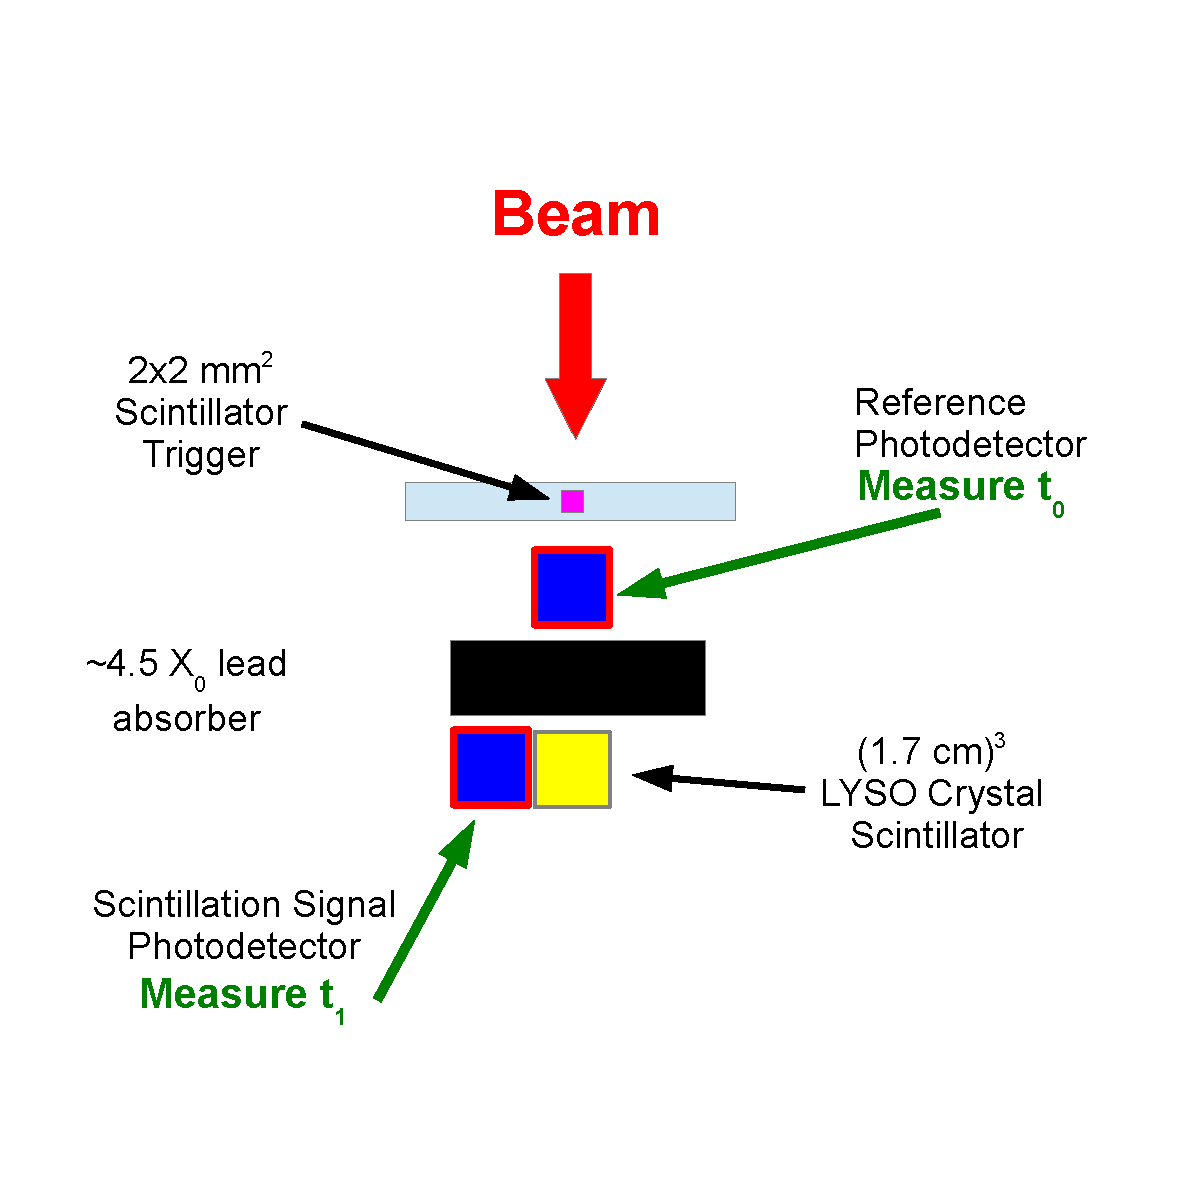
\includegraphics[width=0.45\textwidth]{figs/LYSOSamplingCaloSetupSchematic} 
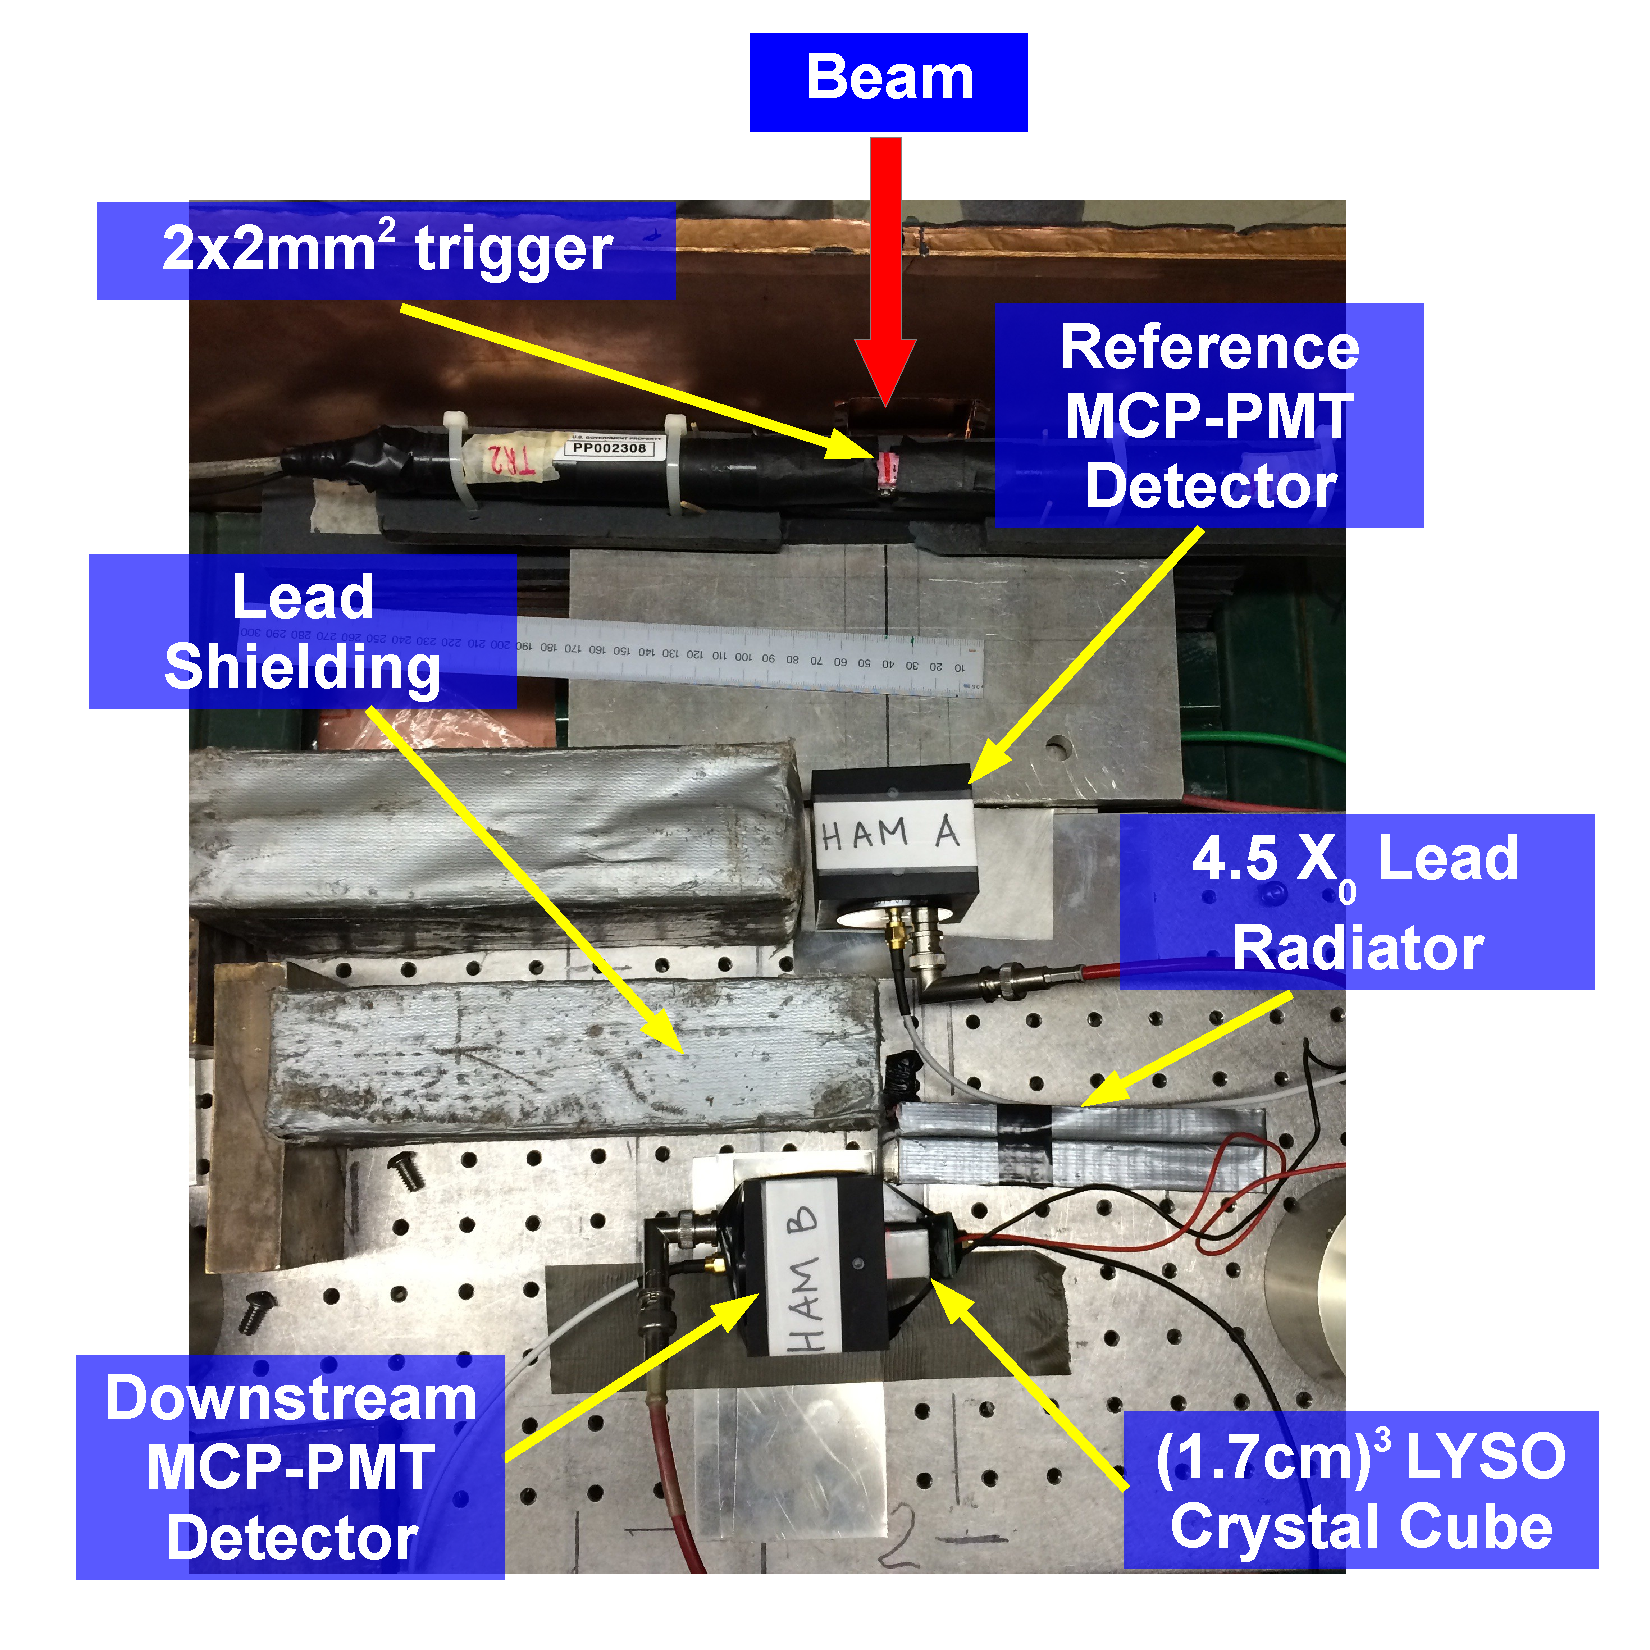
\includegraphics[width=0.45\textwidth]{figs/LYSOSamplingCaloSetupPhoto} 
\caption{ \small A schematic diagram of the experimental setup for the
time of flight measurement using the LYSO sampling calorimeter is shown
on the left, along with a picture of the experimental setup shown on the right. } 
\label{fig:LYSOSamplingCaloSetup}
\end{figure}

To ensure that the electron beam is constrained to within a $2\times 2$~mm$^2$ region, 
a plastic scintillator placed upstream and approximately $2$~mm by $2$~mm in cross sectional 
area is used to trigger the DAQ readout on the DRS  digitizer. Electron events are identified 
by requiring a signal with amplitude larger than $10$~mV in a Cherenkov counter located 
upstream. Large lead bricks are placed upstream of the Hamamatsu R3809 MCP-PMT (HAMB),
out of the path of the beam. These shield the photodetector from stray particles
produced in events where an electromagnetic shower occurs upstream of the lead
radiator. Such stray shower particles yield very fast signals which can
significantly contaminate the scintillation signal. Using the same experimental
setup without the LYSO active element in place, we find that stray shower type
events yield less than $10\%$ contamination and give a negligible effect on the
scintillation signal. 

%The same calorimeter setup with the Photek 240 MCP-PMT in
%place of the Hamamatsu R3809 MCP-PMT, which has an active area about $10$ times
%larger, is found to yield more than $80\%$ contamination and thus does not allow
%a proper measurement of the scintillation signal.

The thickness of the LYSO active element is relatively small and captures only a fraction 
of the total energy of the electron, but yields a reasonable energy measurement
as it is close to the shower maximum.

The time of flight measurement is performed using the LYSO sampling calorimeter
for electron beams with energies varying from $4$~GeV to $32$~GeV. The corresponding 
measured time of flight distributions are shown in Figure~\ref{fig:LYSOCubeTOF}.
We achieve the best time resolution of $34$~ps for electrons
with beam energy of $32$~GeV.

\begin{figure}[ht!] \centering
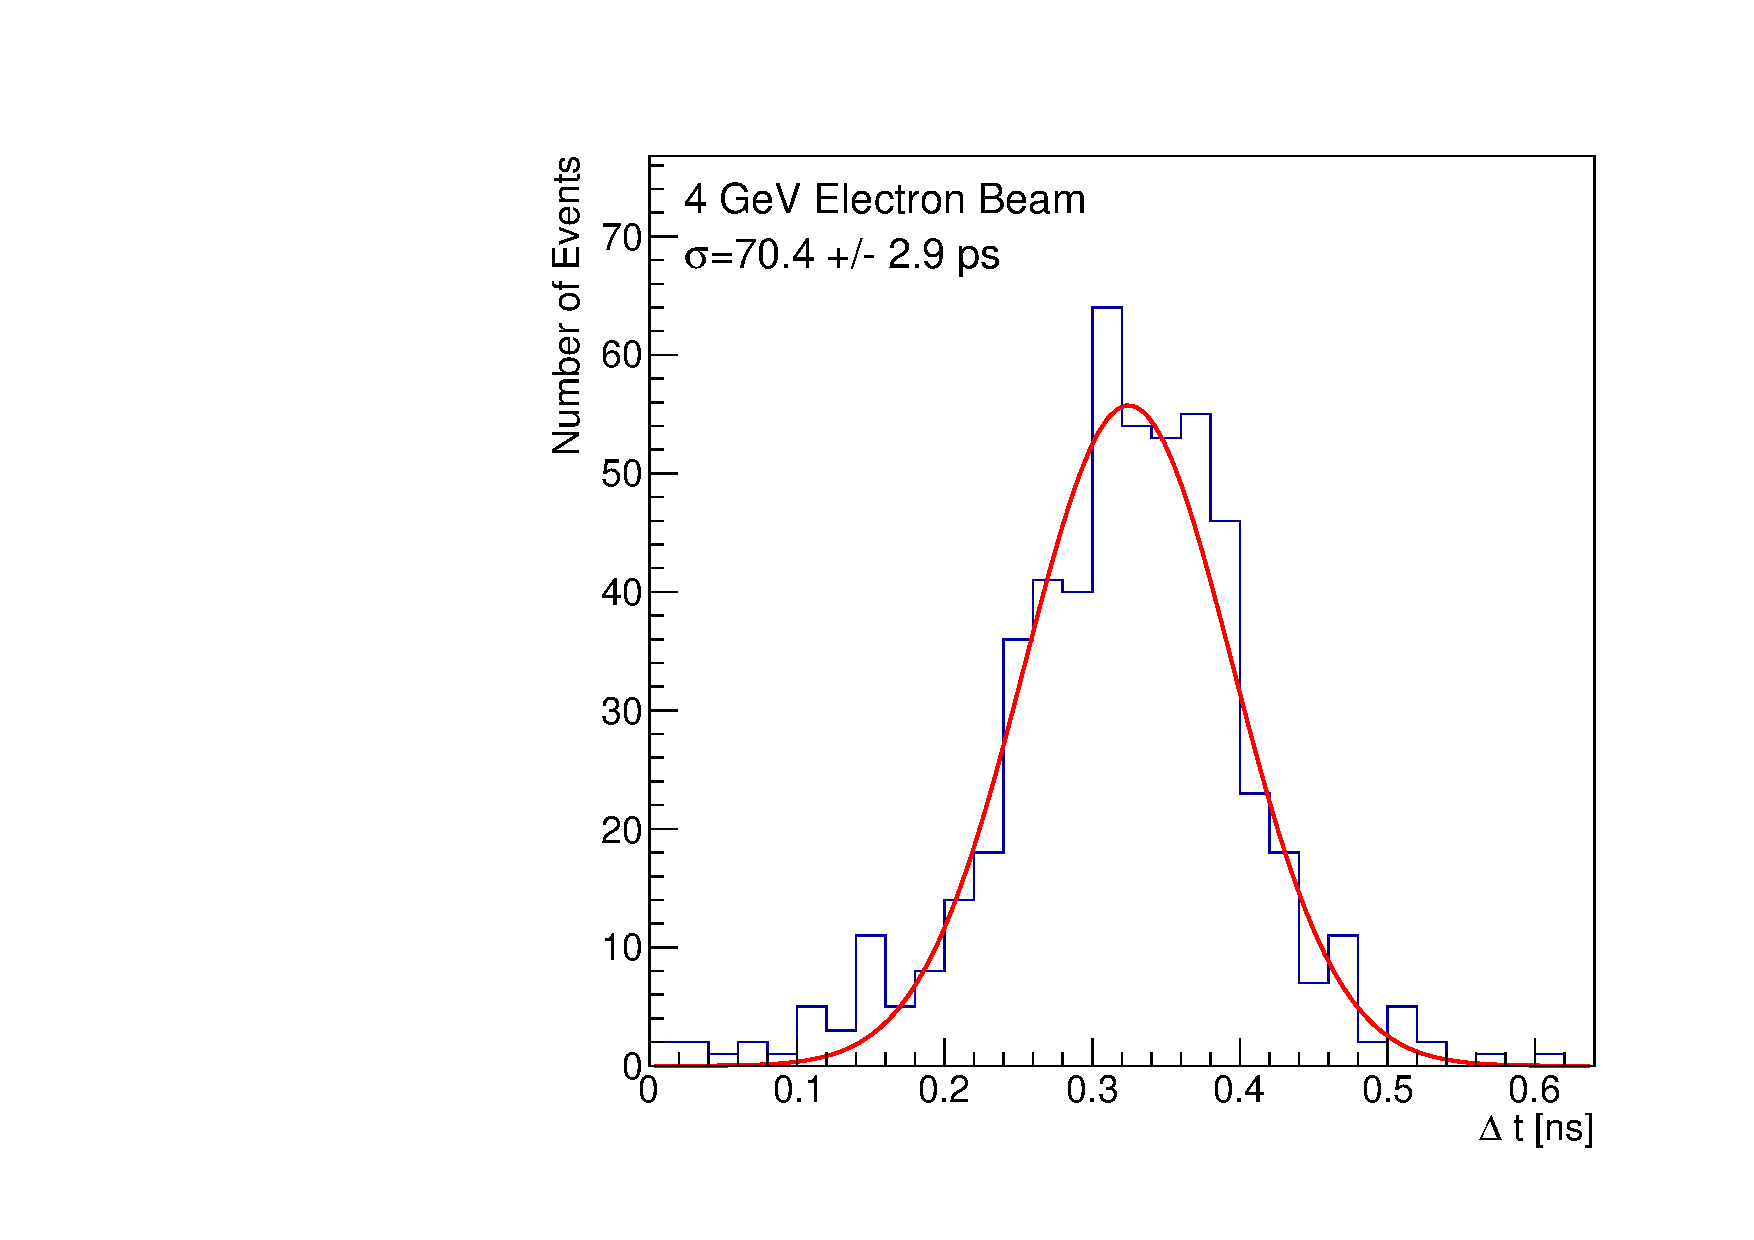
\includegraphics[width=0.23\textwidth]{figs/TOF_Electron_LYSOCube_4GeV} 
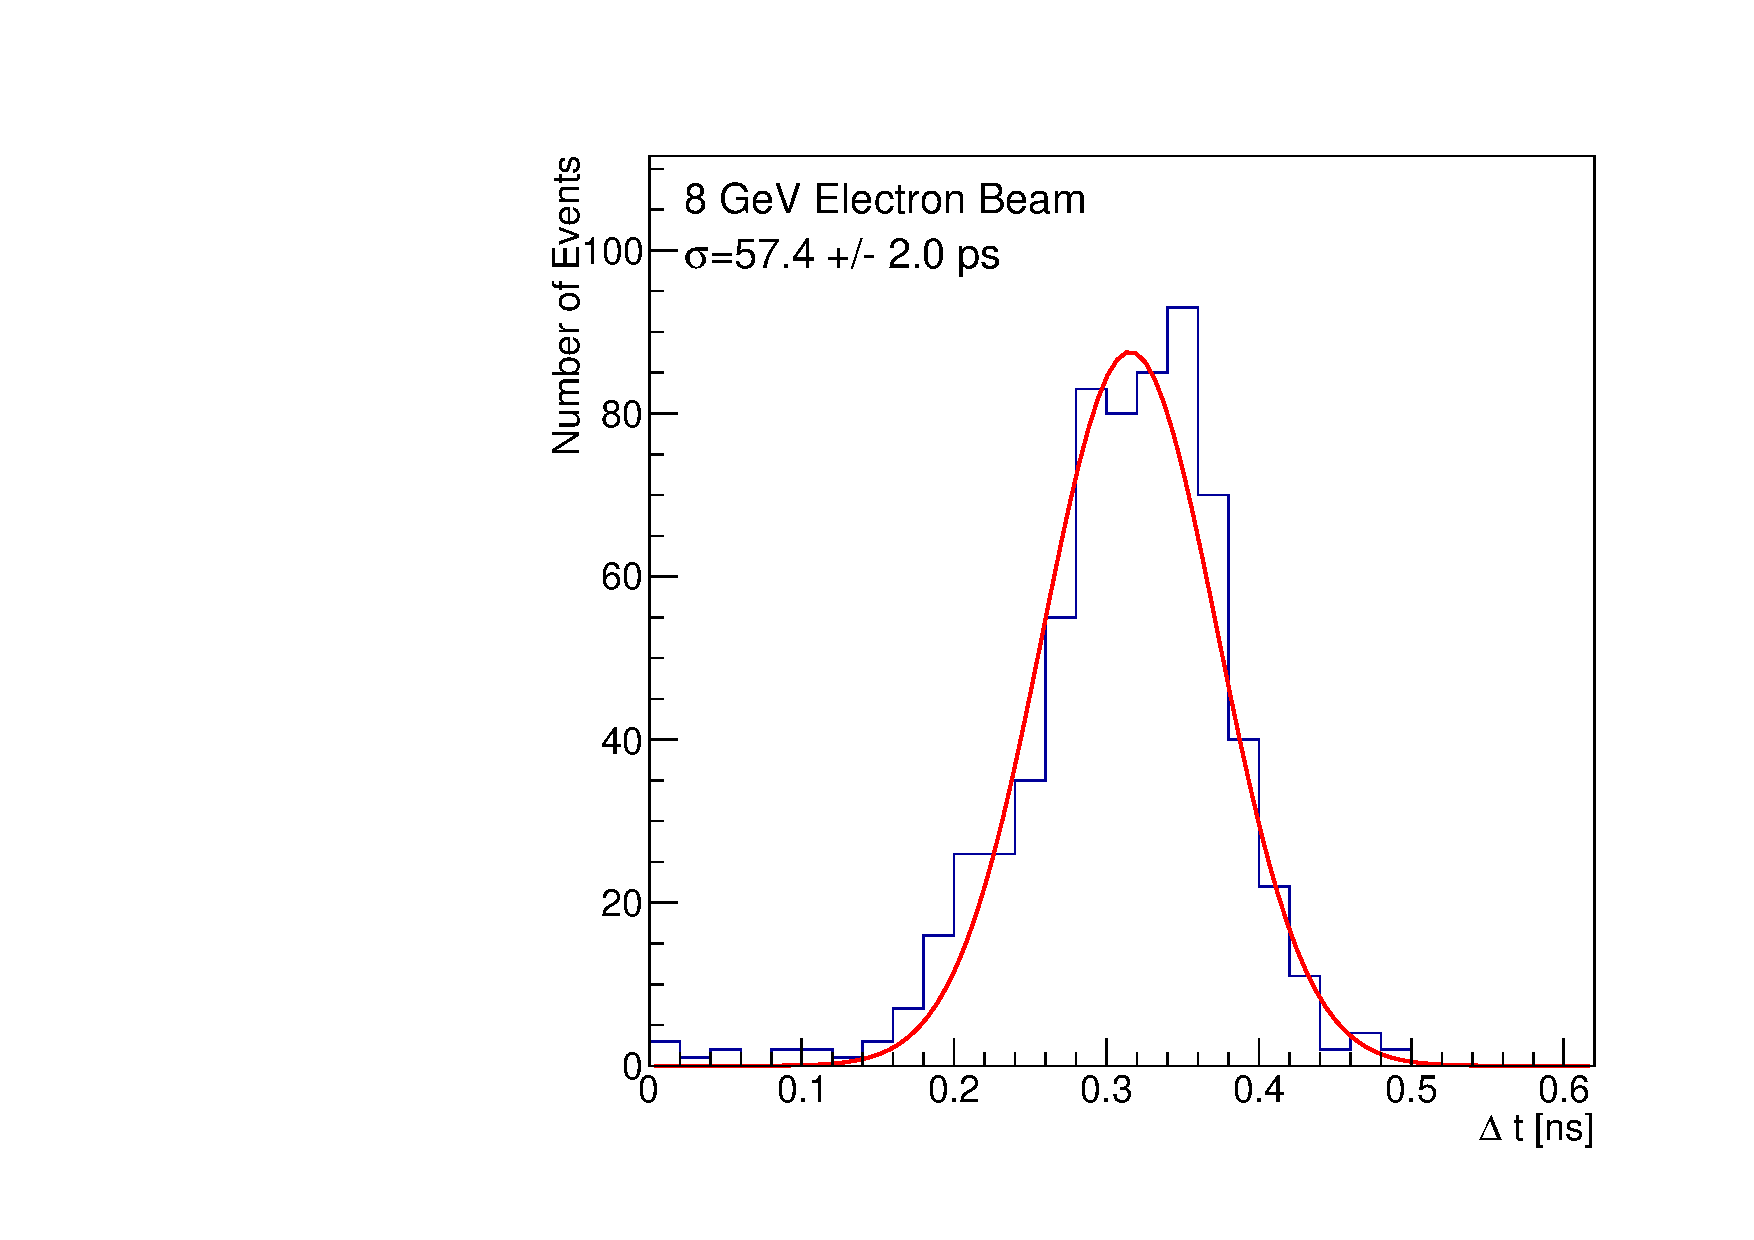
\includegraphics[width=0.23\textwidth]{figs/TOF_Electron_LYSOCube_8GeV} 
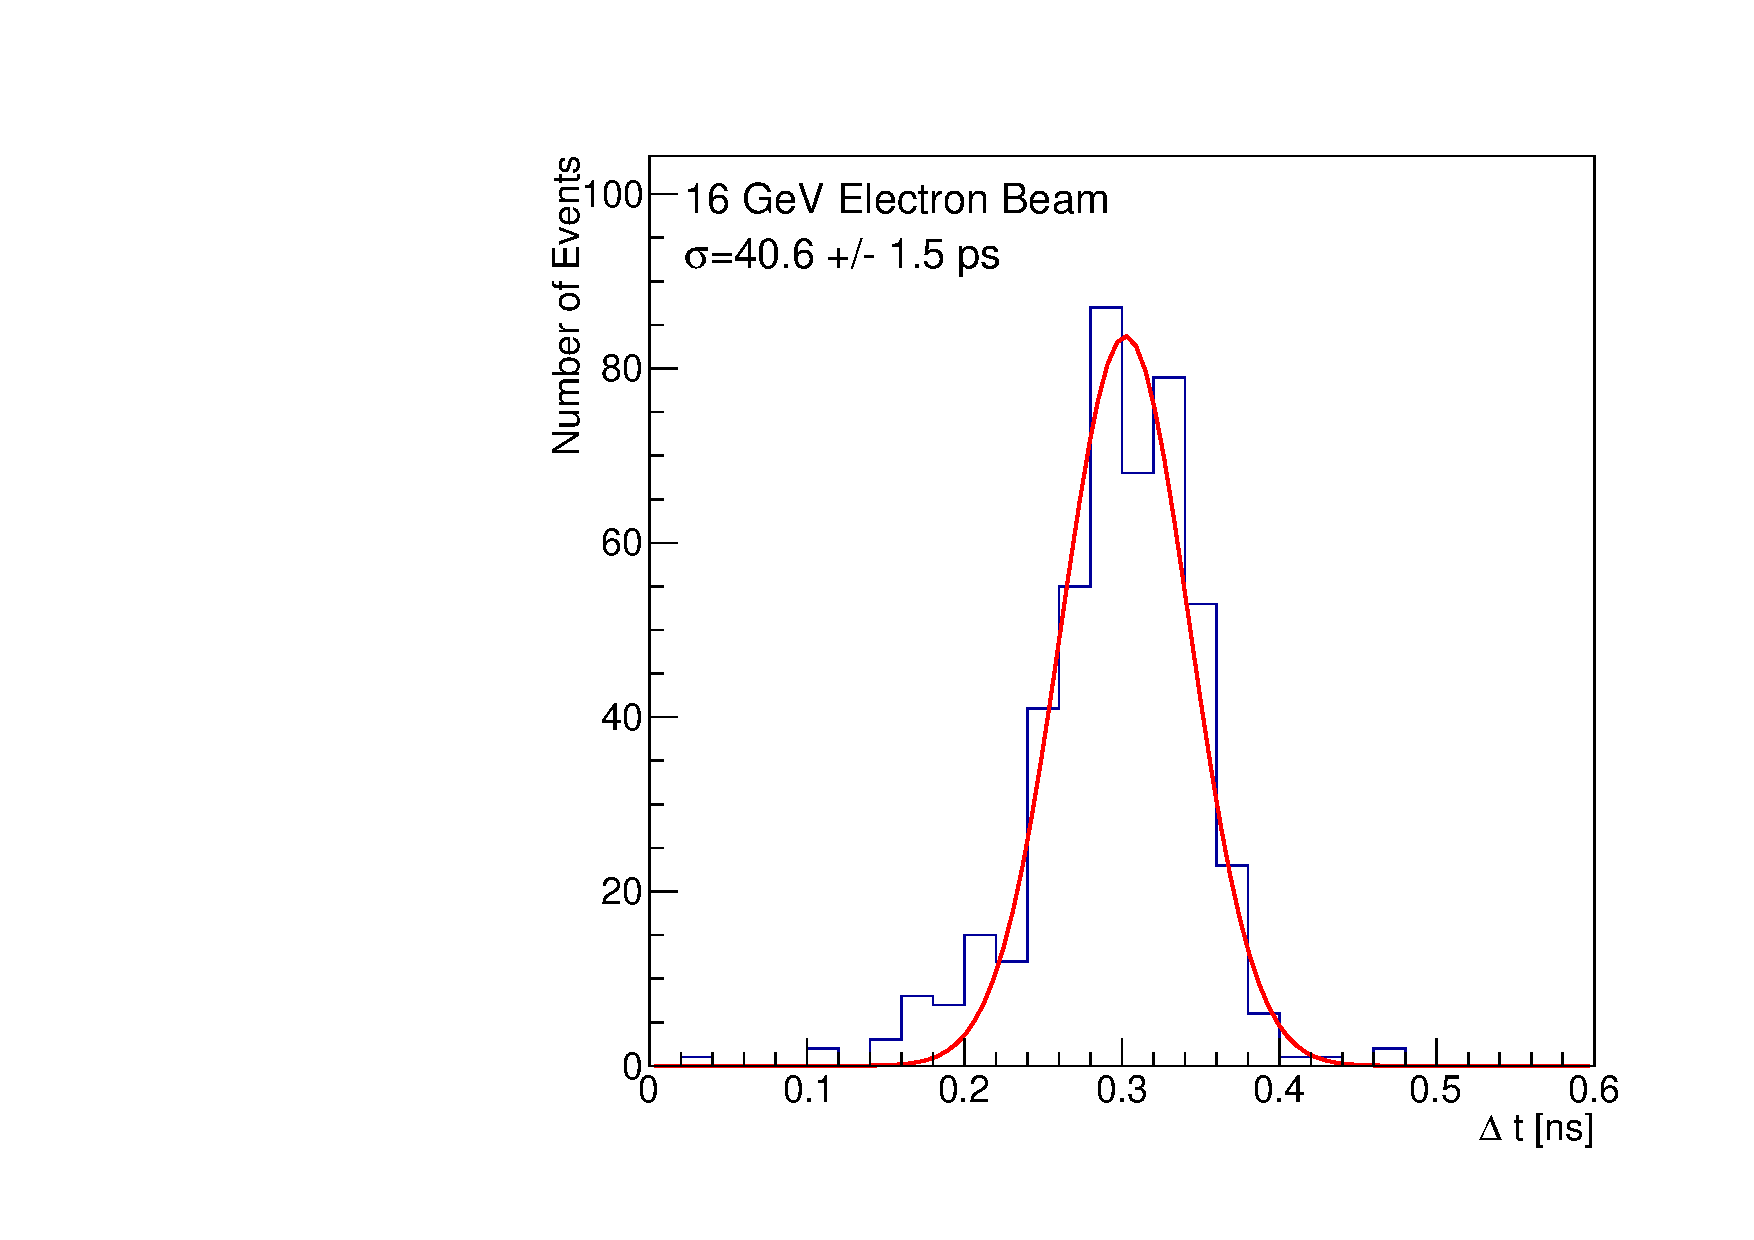
\includegraphics[width=0.23\textwidth]{figs/TOF_Electron_LYSOCube_16GeV} 
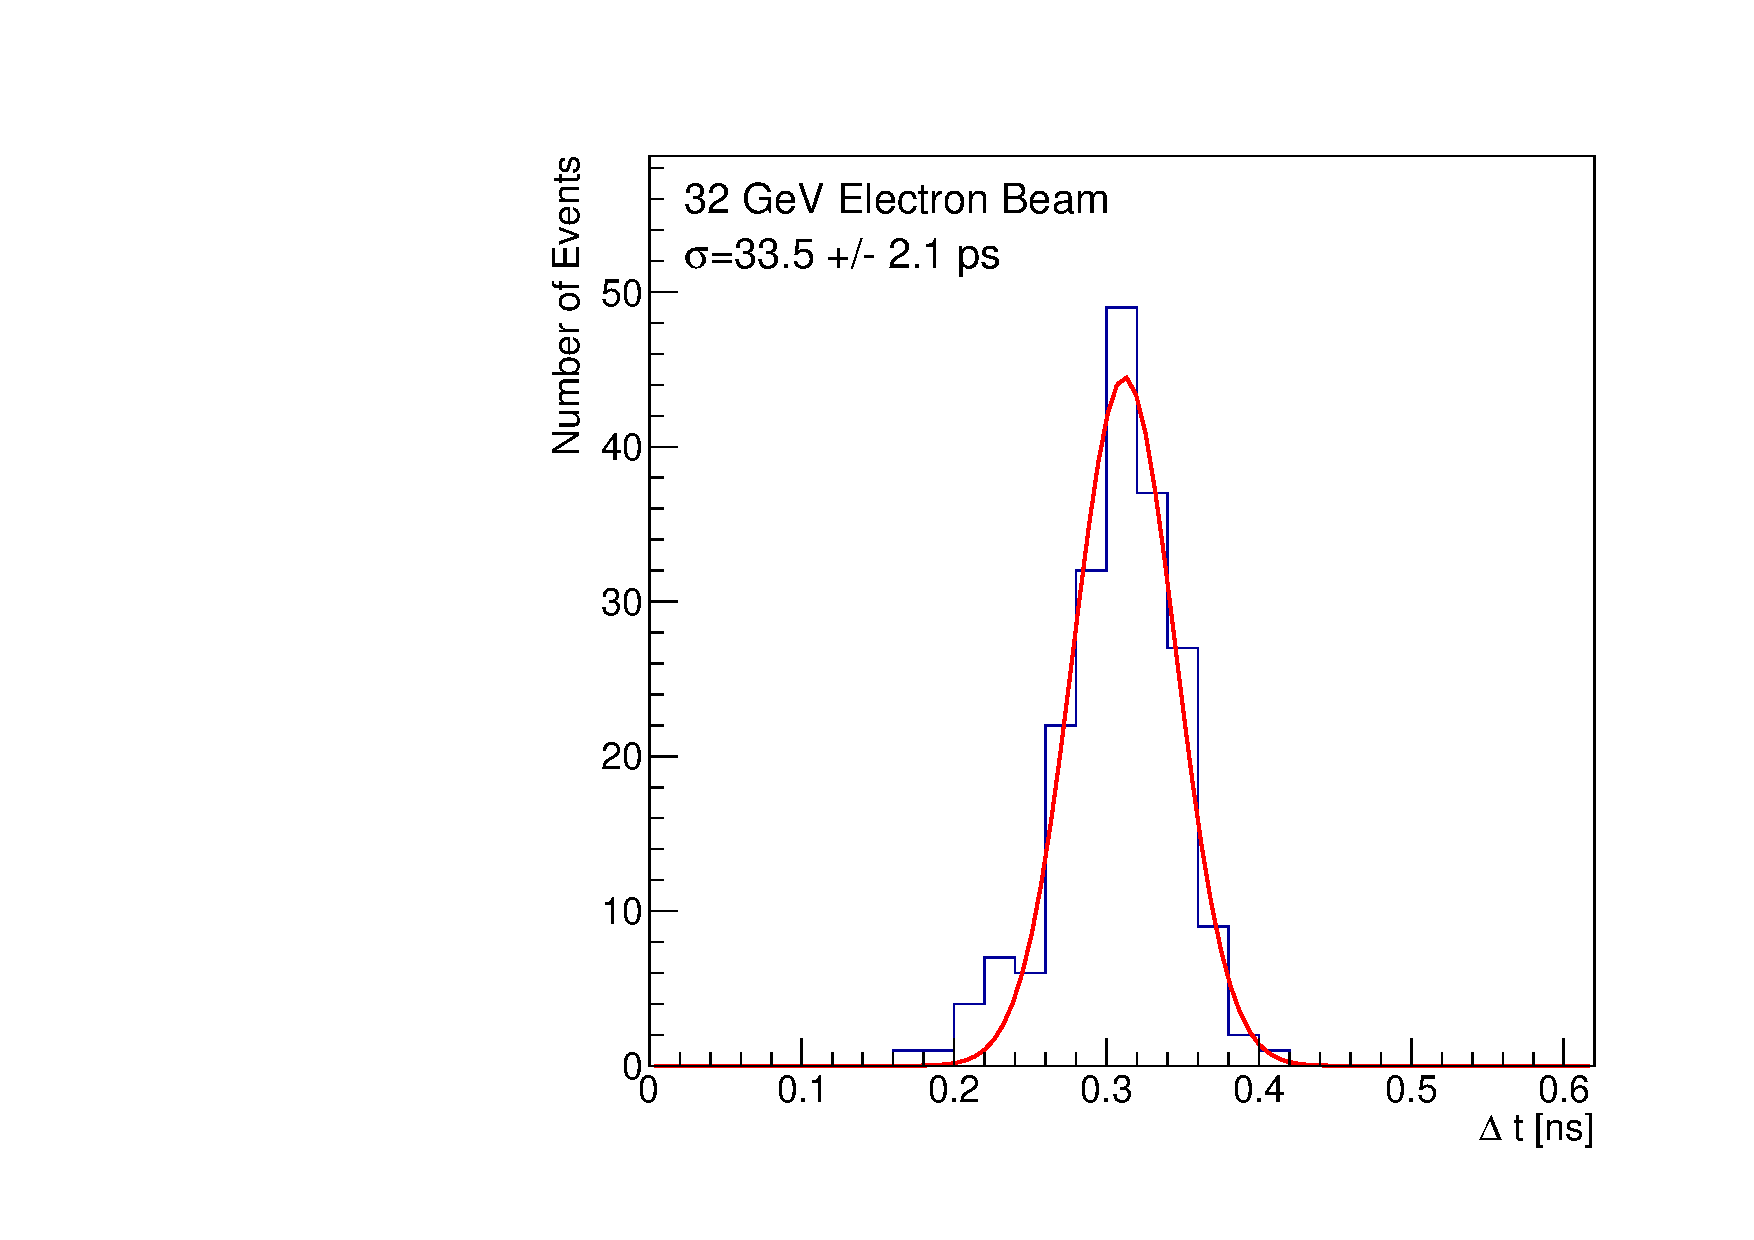
\includegraphics[width=0.23\textwidth]{figs/TOF_Electron_LYSOCube_32GeV} 
\caption{ \small Time of flight distributions for the LYSO cube sampling calorimeter
for 4 GeV (top left), 8 GeV(top right), 16 GeV (bottom left),  32 GeV (bottom right) electron beam energy. } 
\label{fig:LYSOCubeTOF}
\end{figure}

The time resolution measurement is plotted as a function of the
beam energy in Figure~\ref{fig:LYSOCubeTOFResolutionVsEnergy} (left). We fit the result to the sum of a 
$1/\sqrt{E}$ term and a constant term of about $11$~ps.   Given that we measure the contribution 
to the intrinsic time resolution of the photodetector and the DAQ electronics to be about 
$20$~ps~\cite{MCPFastCaloNIMA}, using the results from the 32 GeV electron beam, we infer 
that the combined contribution to the time resolution from the shower profile
fluctuations, the scintillation mechanism, and the light propagation time inside the
LYSO cube is about $27$~ps.  

\subsection{Timing Studies of the LYSO-Tungsten Shashlik Calorimeter}
\subsubsection{Wavelength shifting fibers readout (WLS Y11 \& DSB1)}
We study the time resolution of a LYSO-tungsten Shashlik calorimeter, one of the
proposed choices for the Phase 2 upgrade of the CMS endcap calorimeter
system~\cite{Contardo:1605208}. We compare the time resolution performance for
two alternative light propagation schemes. 

In our setup the scintillation light is collected by WLS fibers that
pass through a set of four holes in the LYSO and tungsten layers. In 
Figure~\ref{fig:ShashlikDiagram}, a shashlik cell and the light extraction 
scheme is illustrated. A schematic diagram and a photograph showing this experimental
setup are shown in Figure~\ref{fig:ShashlikFiberSetup}. Two MCP-PMTs  by 
Hamamatsu (R3809) are used to collect the scintillation light, while a Photek 240 
MCP-PMT is used as a reference time detector. 

\begin{figure}[ht!] \centering
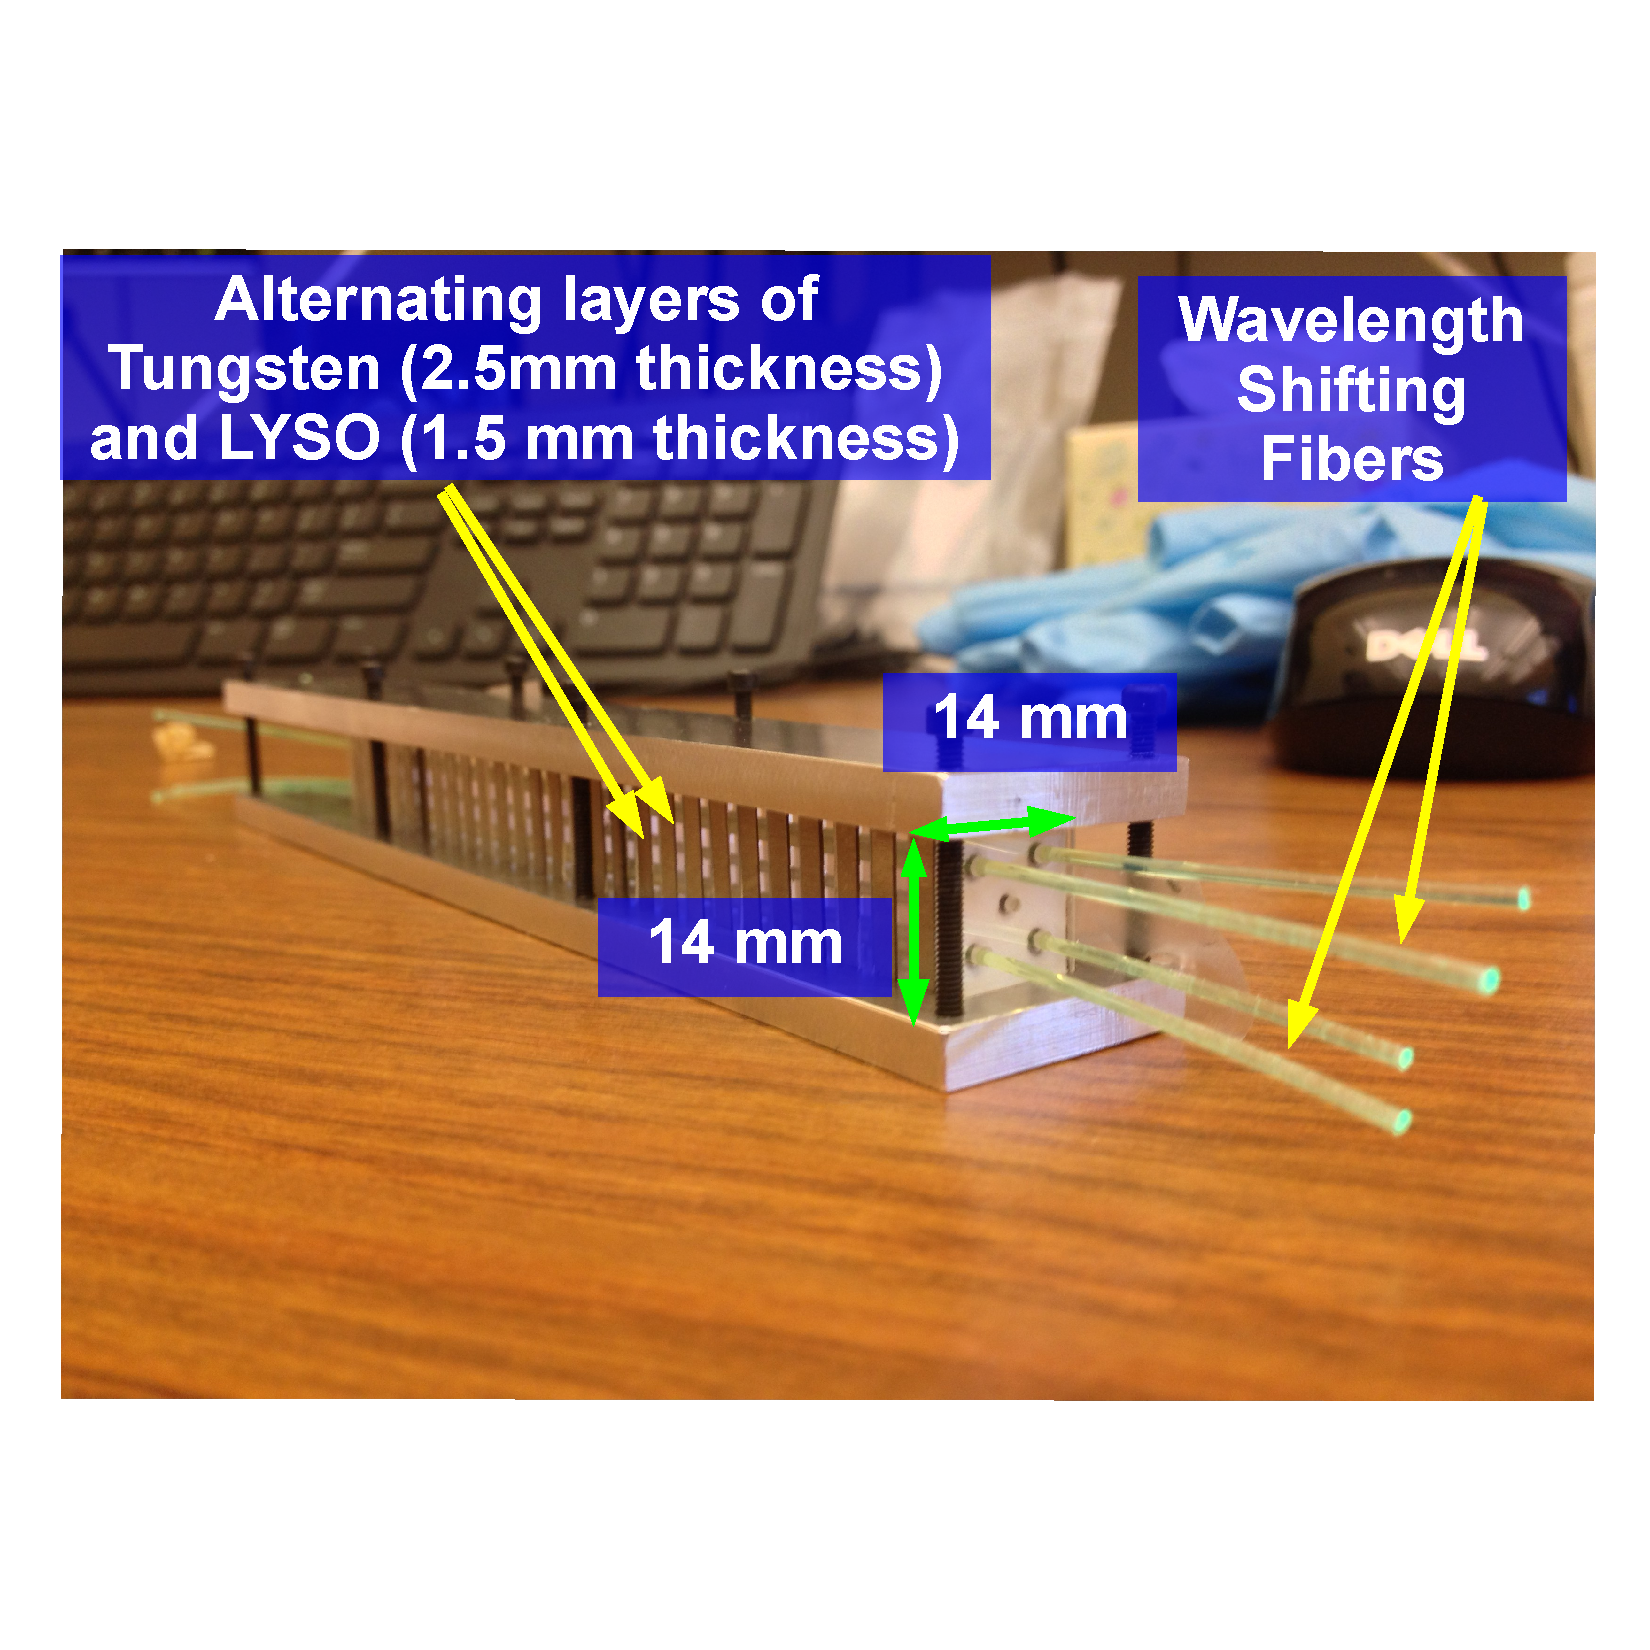
\includegraphics[width=0.6\textwidth]{figs/ShashlikCellPhoto.pdf} 
\caption{\small The shashlik configuration based upon interleaved W and LYSO layers. 
Twenty-eight LYSO crystal plates and twenty-seven W plates comprise the module.
Four WLS fibers are used to read out the scintillation light from the 
tiles. } 
\label{fig:ShashlikDiagram}
\end{figure}

\begin{figure}[ht!] \centering
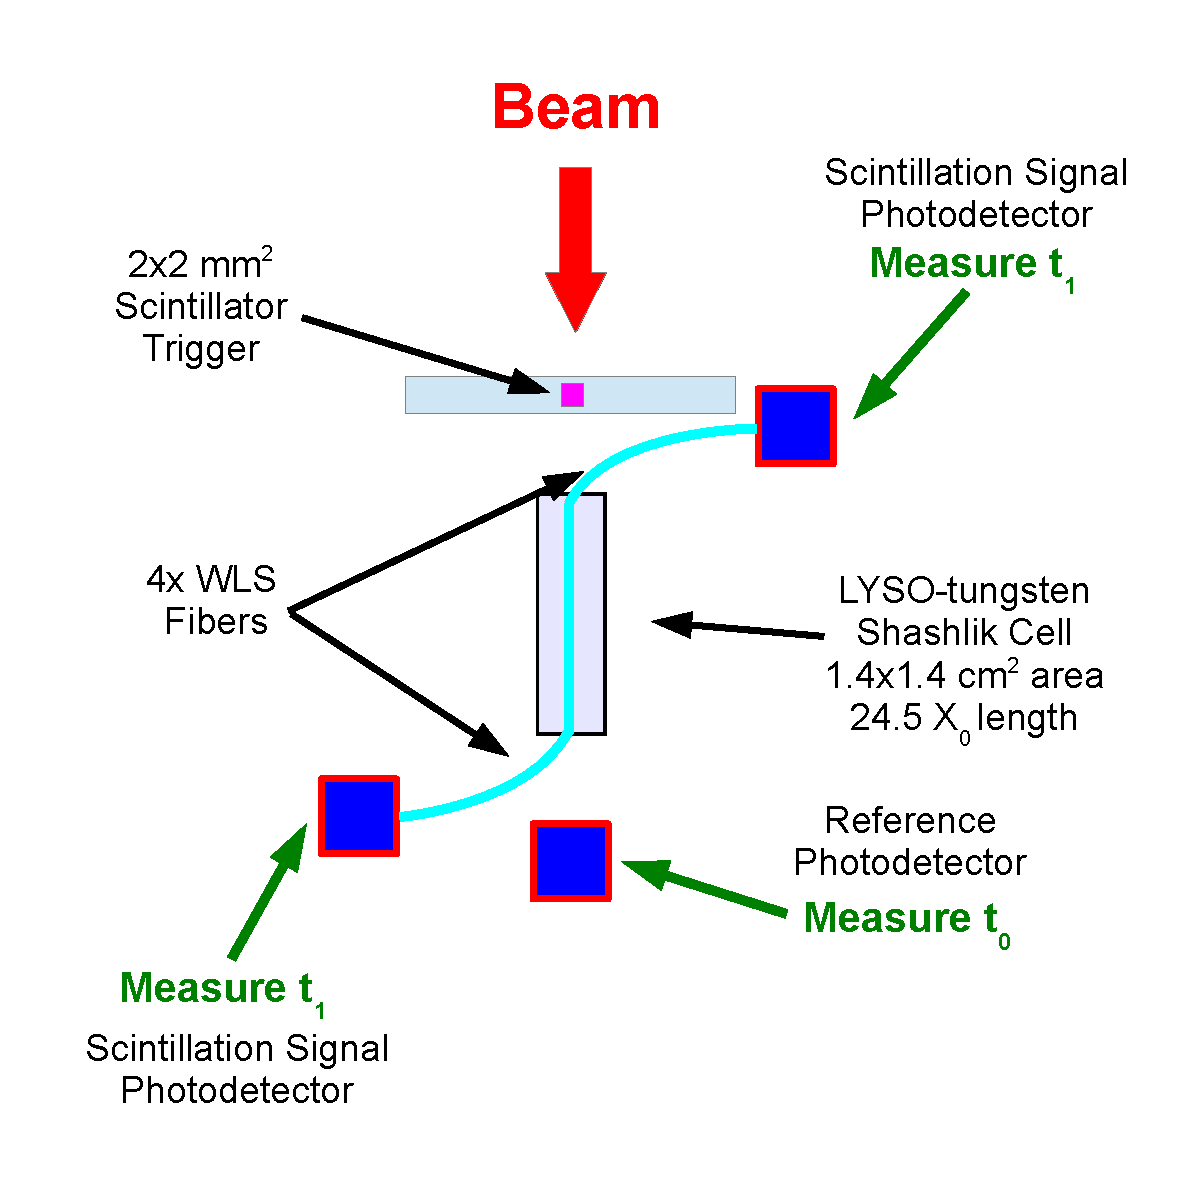
\includegraphics[width=0.45\textwidth]{figs/ShashlikFiberSetupSchematic} 
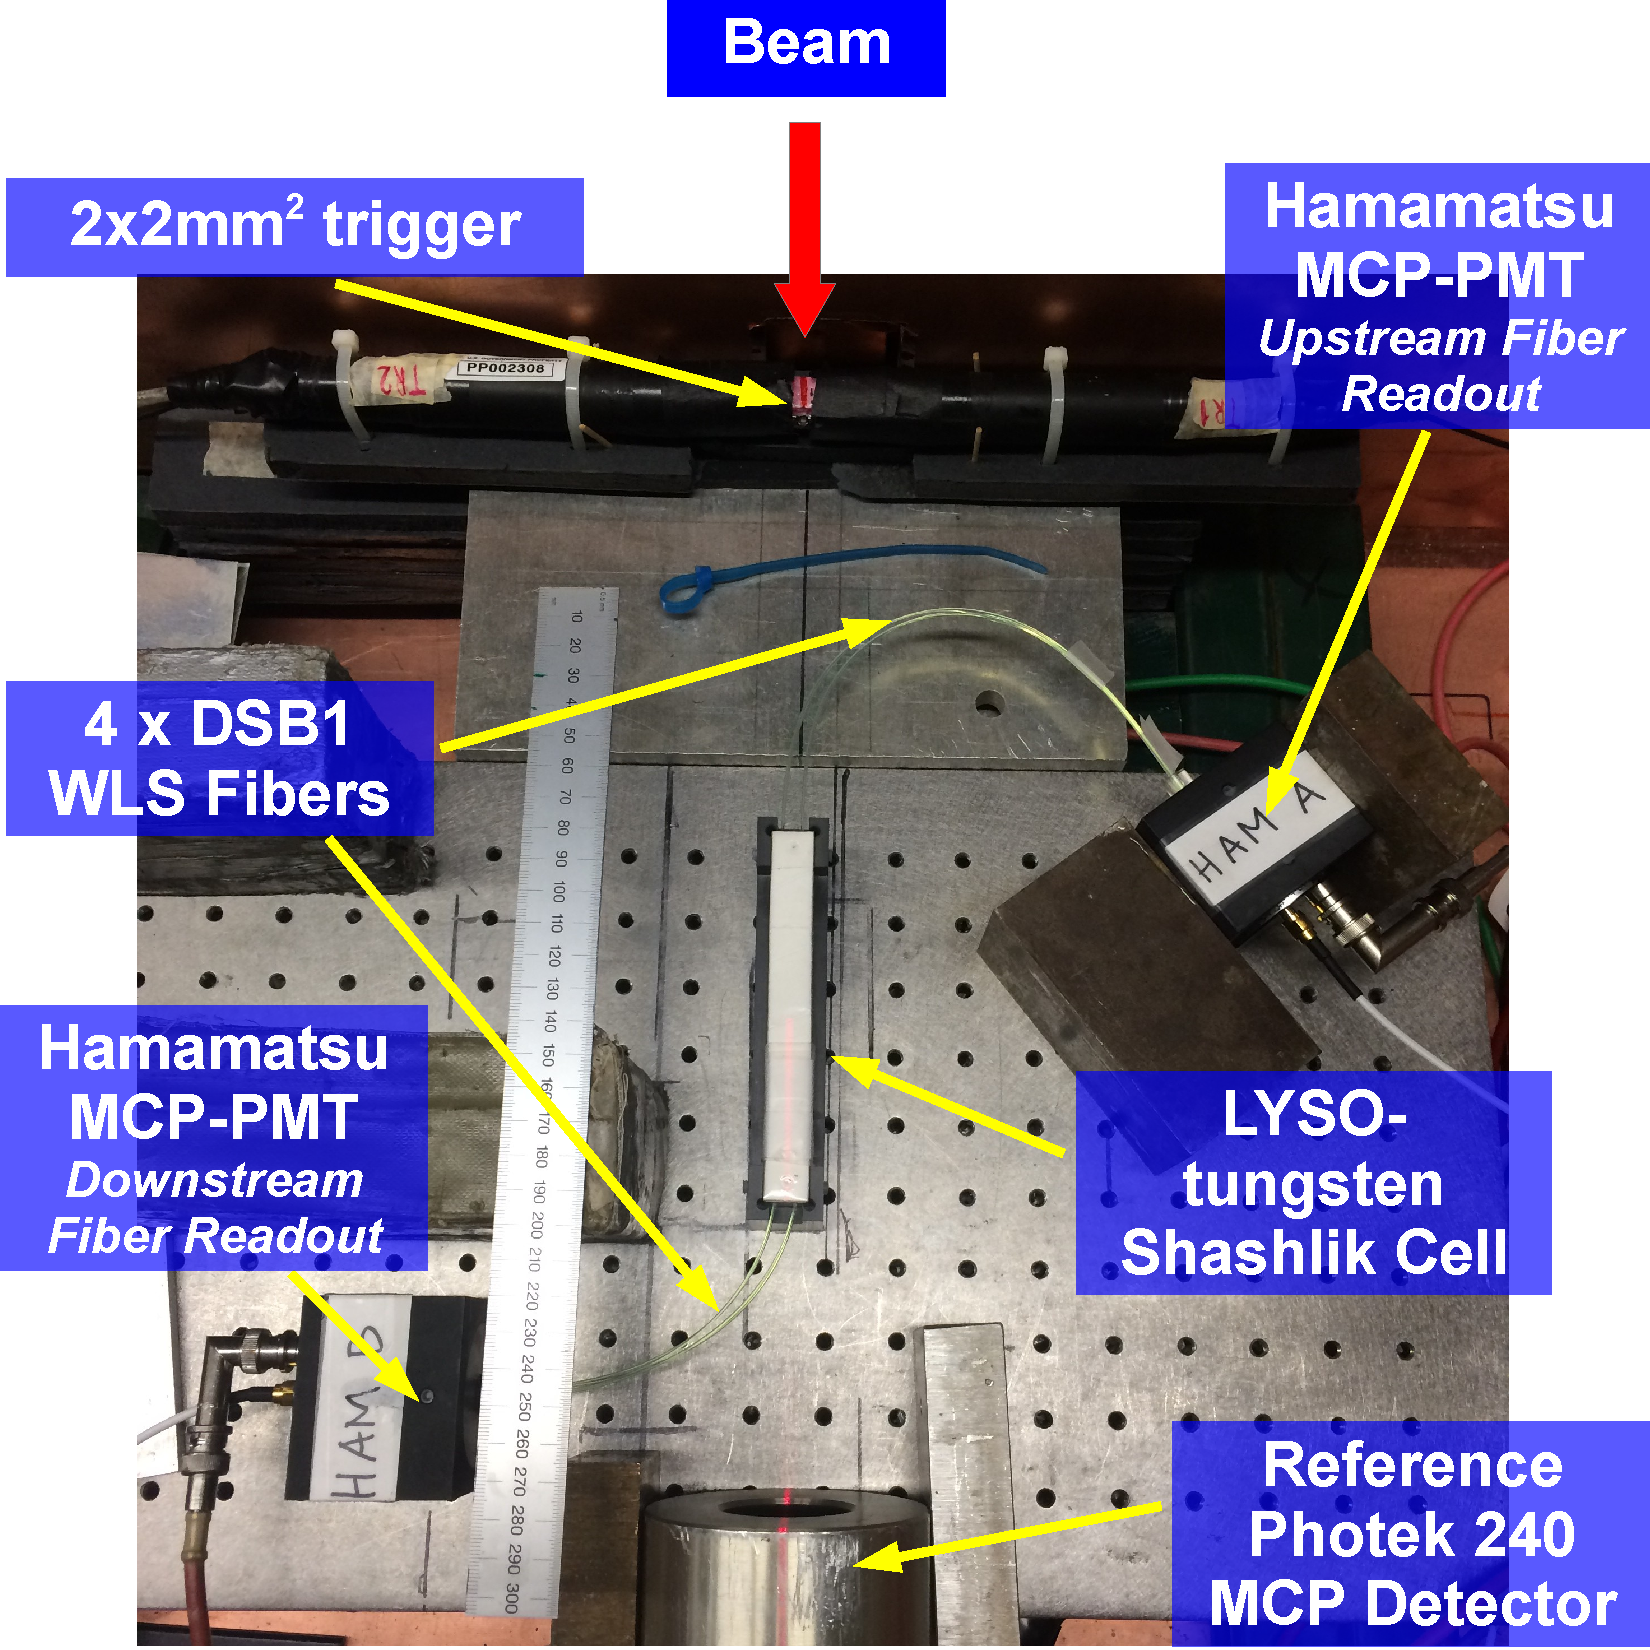
\includegraphics[width=0.45\textwidth]{figs/ShashlikFiberSetupPhoto} 
\caption{\small A schematic diagram of the experimental setup for the
time of flight measurement using the LYSO-tungsten shashlik calorimeter
with fiber signal extraction, along with a photograph of the
experimental setup. } 
\label{fig:ShashlikFiberSetup}
\end{figure}

%In this setup the wavelength shifting mechanism in the fibers affects the rise
%time and time jitter of the final signal pulse.
 %We investigate this effect in
%greater detail by 
 We compare the signal pulses obtained using two different
 types of WLS fiber in the same LYSO-tungsten shashlik calorimeter. In
 Figure~\ref{fig:FiberPulseComparison} (a) and (b) and we show the pulse shapes
 averaged over a few hundred events obtained using DSB1 fibers~\cite{Albrecht}
 and Y11 fibers, plotted in blue and red respectively. We find that the rise
 time of the pulse obtained using the DSB1 fibers, about $2.4$~ns, is
 significantly faster than the rise time of the pulse obtained using the Y11
 fibers, which is about $7.1$~ns. To optimize the time resolution of this type
 of calorimeter the DSB1 fiber provides a better choice than Y11 if only this
 parameter is considered. The signal rise times we observe are comparable to the
 measured decay times of the corresponding WLS fibers~\cite{Albrecht}. 
 
% compared
% with the average pulse shape obtained from direct optical coupling of the
% photodetector to the edge of one of the LYSO tiles, plotted in green. 
%


\begin{figure}[ht!] \centering
%\includegraphics[width=0.32\textwidth]{figs/FiberPulsesY11DSB1} 
%
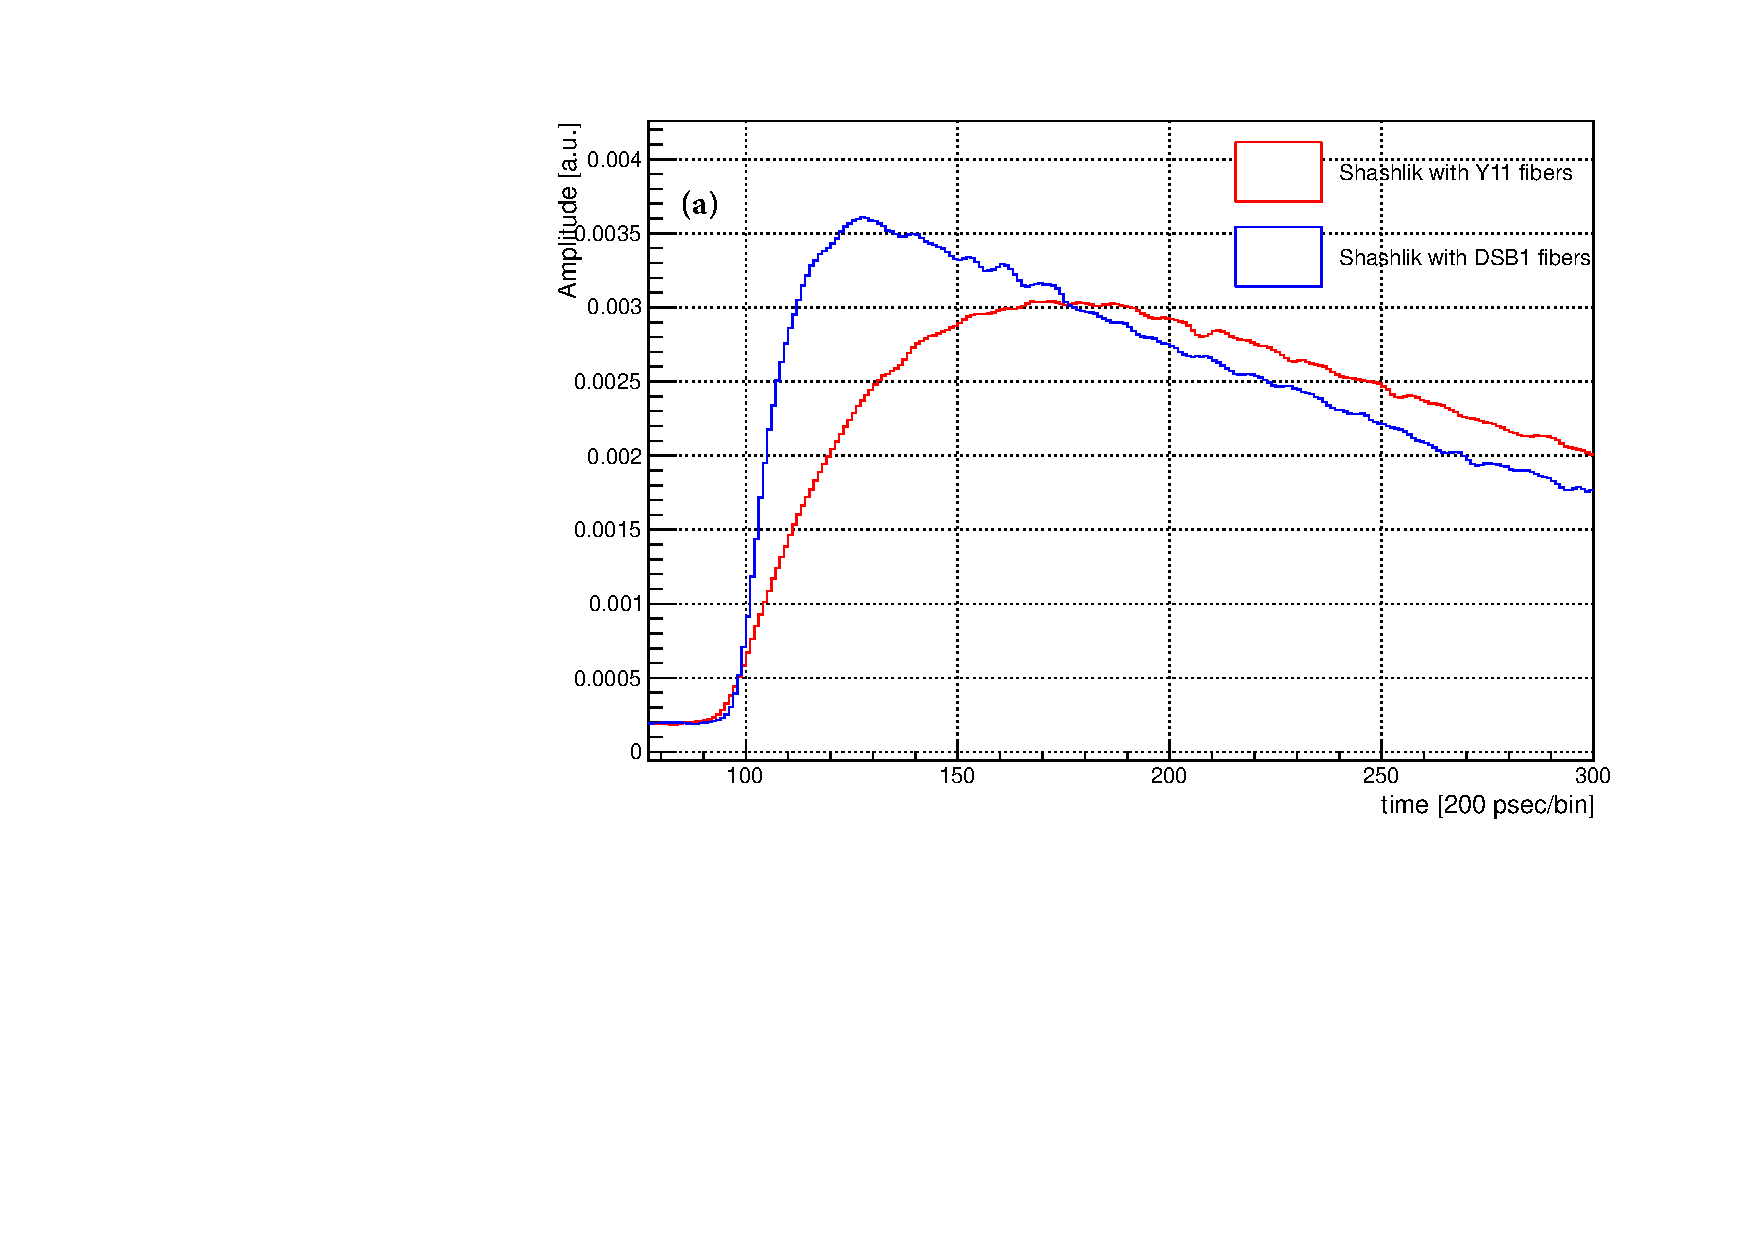
\includegraphics[width=0.48\textwidth]{figs/FiberPulsesZoomY11DSB1} 
%
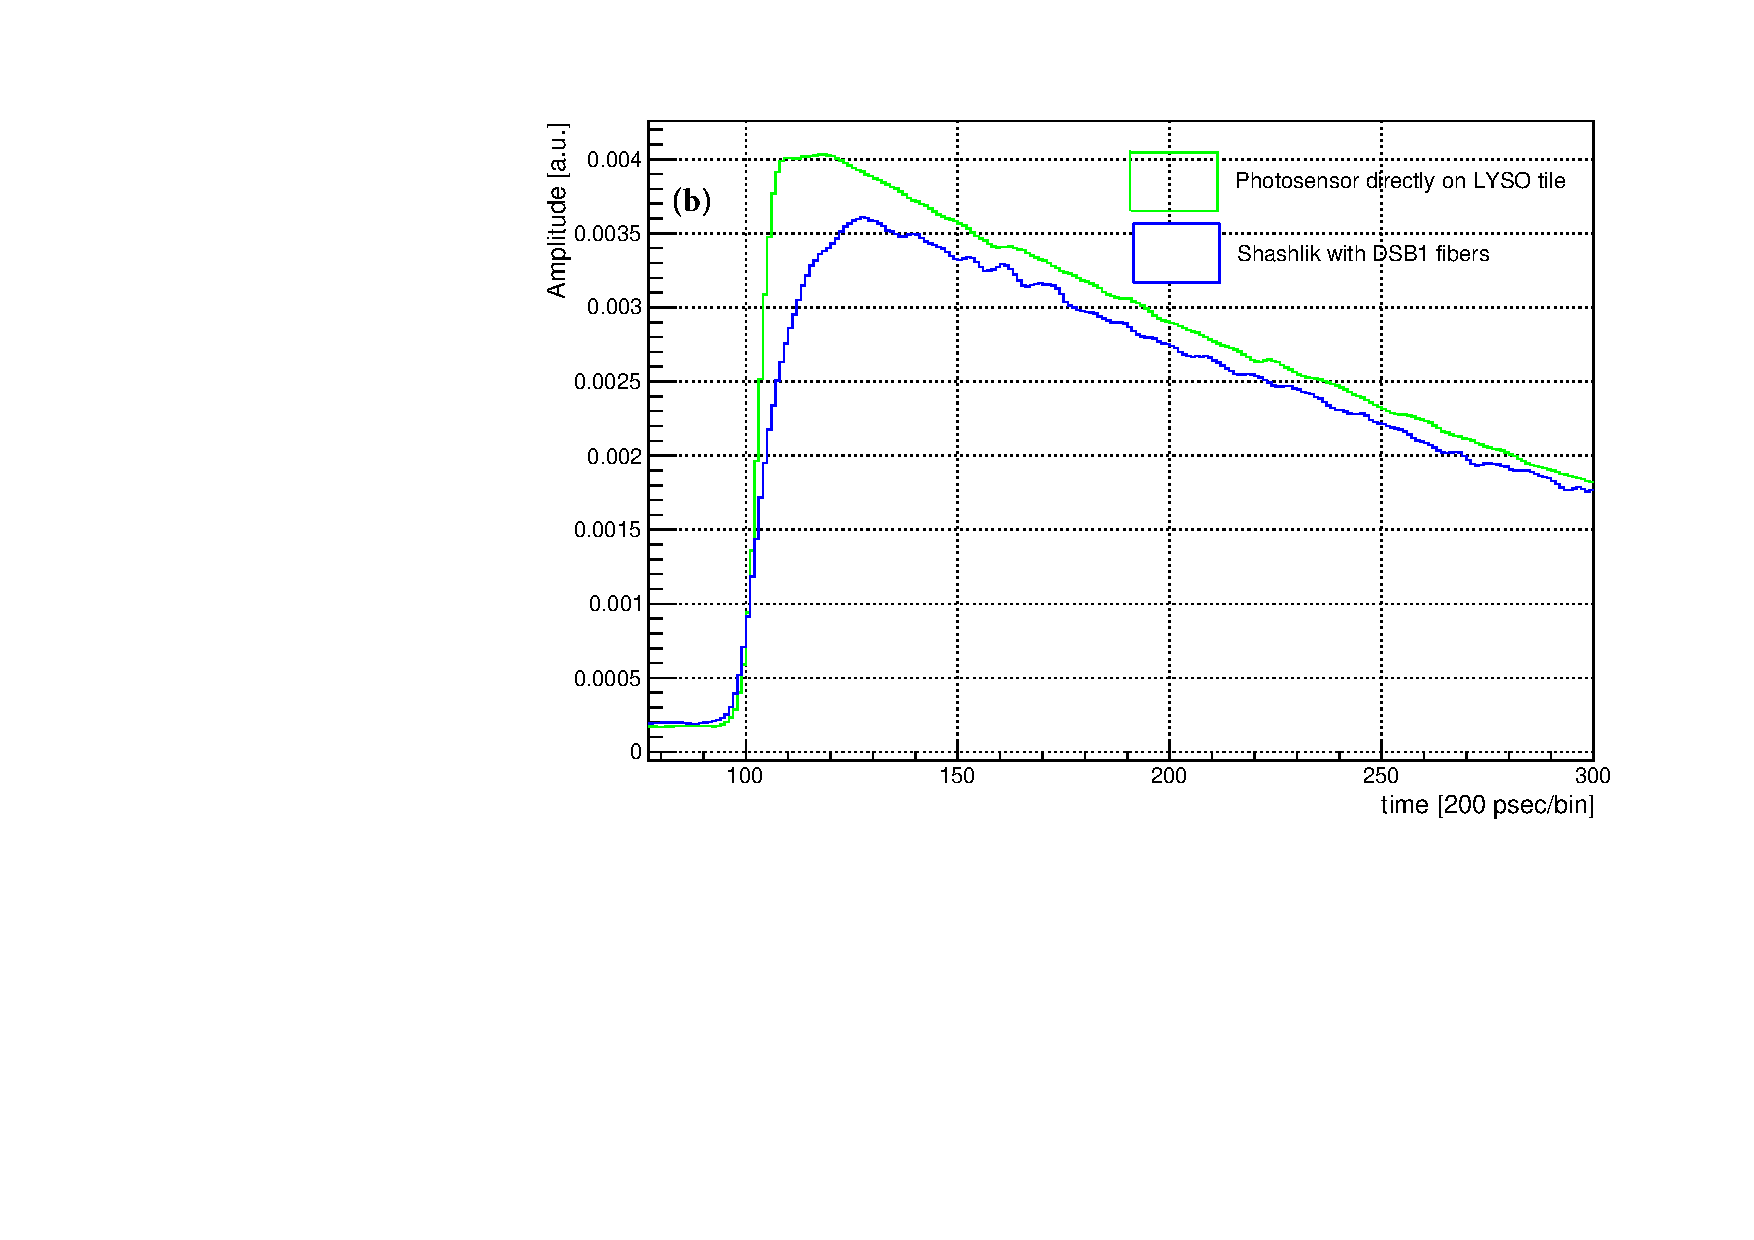
\includegraphics[width=0.48\textwidth]{figs/FiberPulsesZoomDirectDSB1} 
%
\caption{\small (a) Pulse shapes digitized by the DRS4 board and averaged over several hundred events 
obtained from the LYSO-tungsten shashlik calorimeter with light extracted using
DSB1 (blue) and Y11 (red) WLS fibers. 
 (b)  DSB1(blue) shashlik average light pulse shape compared with 
the averaged pulse shape obtained from direct optical coupling of the photodetector to one edge of  a LYSO tile in the shashlik calorimeter.  (green)} 
\label{fig:FiberPulseComparison}
\end{figure}


Using the shashlik calorimeter cell with DSB1 fibers, we measure the time resolution
for electron beams with energy varying between $4$~GeV and $32$~GeV.
In Figure~\ref{fig:ShashlikFiberEnergy32GeV} (b) we show the distribution
of the pulse integral which is proportional to the total collected charge,
for the $32$~GeV beam, and observe an energy resolution of about $5\%$
while for the small LYSO cube shown in ~\ref{fig:ShashlikFiberEnergy32GeV} (a),  the energy 
resolution was about 20\%. For this particular run in the Shashlik setup, no electron identification 
requirements could be made due to a misconfiguration of the upstream Cherenkov counter, 
so the background is visible.


Time of flight distributions, fitted to gaussian functions,
are shown in Figure~\ref{fig:ShashlikFiberTOF}, and the 
$\sigma$ parameter of the gaussian fit is plotted as a function of the
beam energy in Figure~\ref{fig:ShashlikSideReadoutTOFResolutionVsEnergy}.
We find that the dependence of the time resolution on
beam energy follows a $1/\sqrt{E}$ functional form, indicating
that the current calorimeter setup remains in the photostatistics limited regime. 
The best time resolution we obtain with this setup is $104$~ps. As the measurements are 
photostatistics limited, the result can be improved in the future if the light collection
efficiency is increased.
\begin{figure}[ht!] \centering
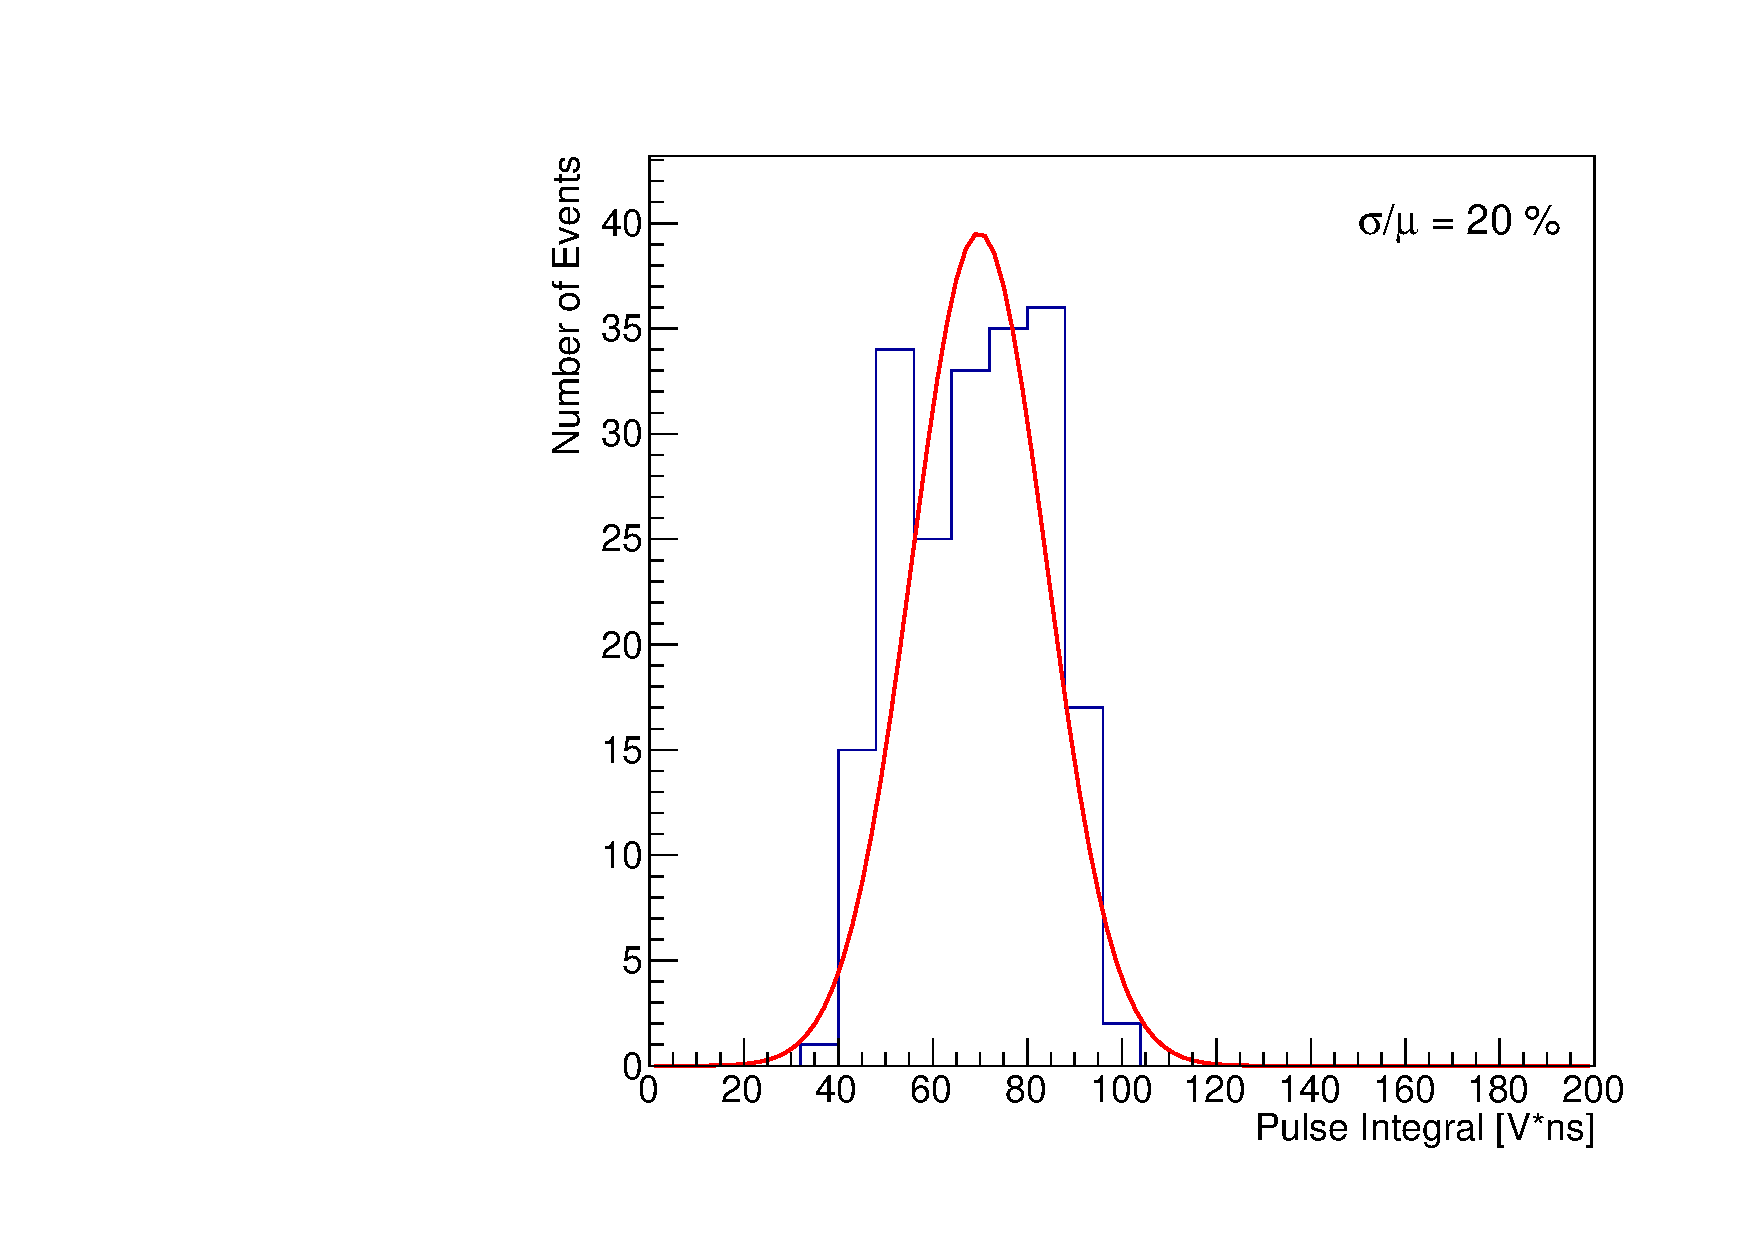
\includegraphics[width=0.45\textwidth]{figs/TOF_Electron_LYSOCube_32GeV_energy} 
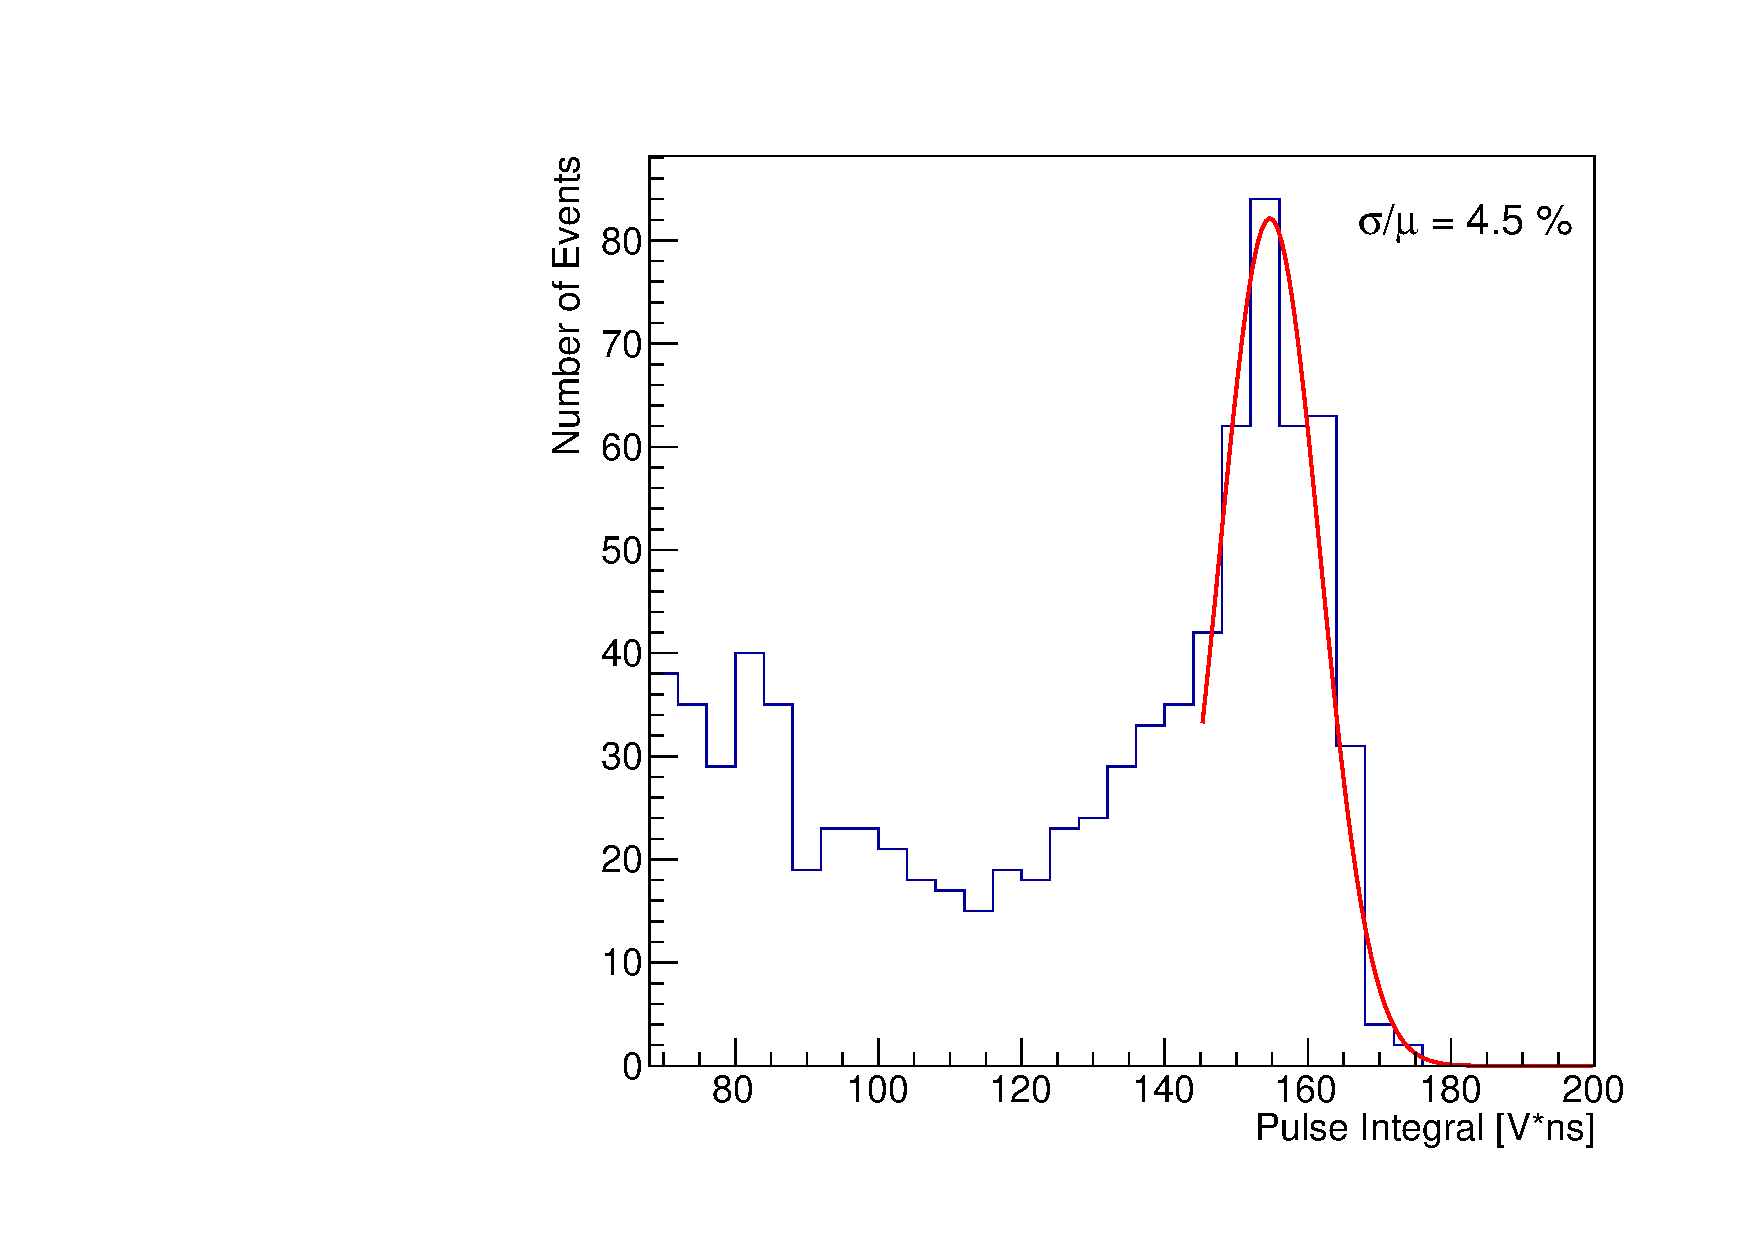
\includegraphics[width=0.45\textwidth]{figs/TOF_ShashlikDSB1Fiber_Electron_32GeV_energy} 
\caption{ (Left) Histogram of the pulse integral which is proportional to the
total collected charge is shown for events recorded using the LYSO cube sampling
calorimeter for a $32$~GeV electron beam. (Right) Histogram of the pulse
integral for events recorded using the LYSO-tungsten shashlik calorimeter using
DSB1 fibers, for a $32$~GeV electron beam. The background is included due to a
misconfiguration of the Cherenkov counter. } 
\label{fig:ShashlikFiberEnergy32GeV}
\end{figure}

\begin{figure}[ht!] \centering
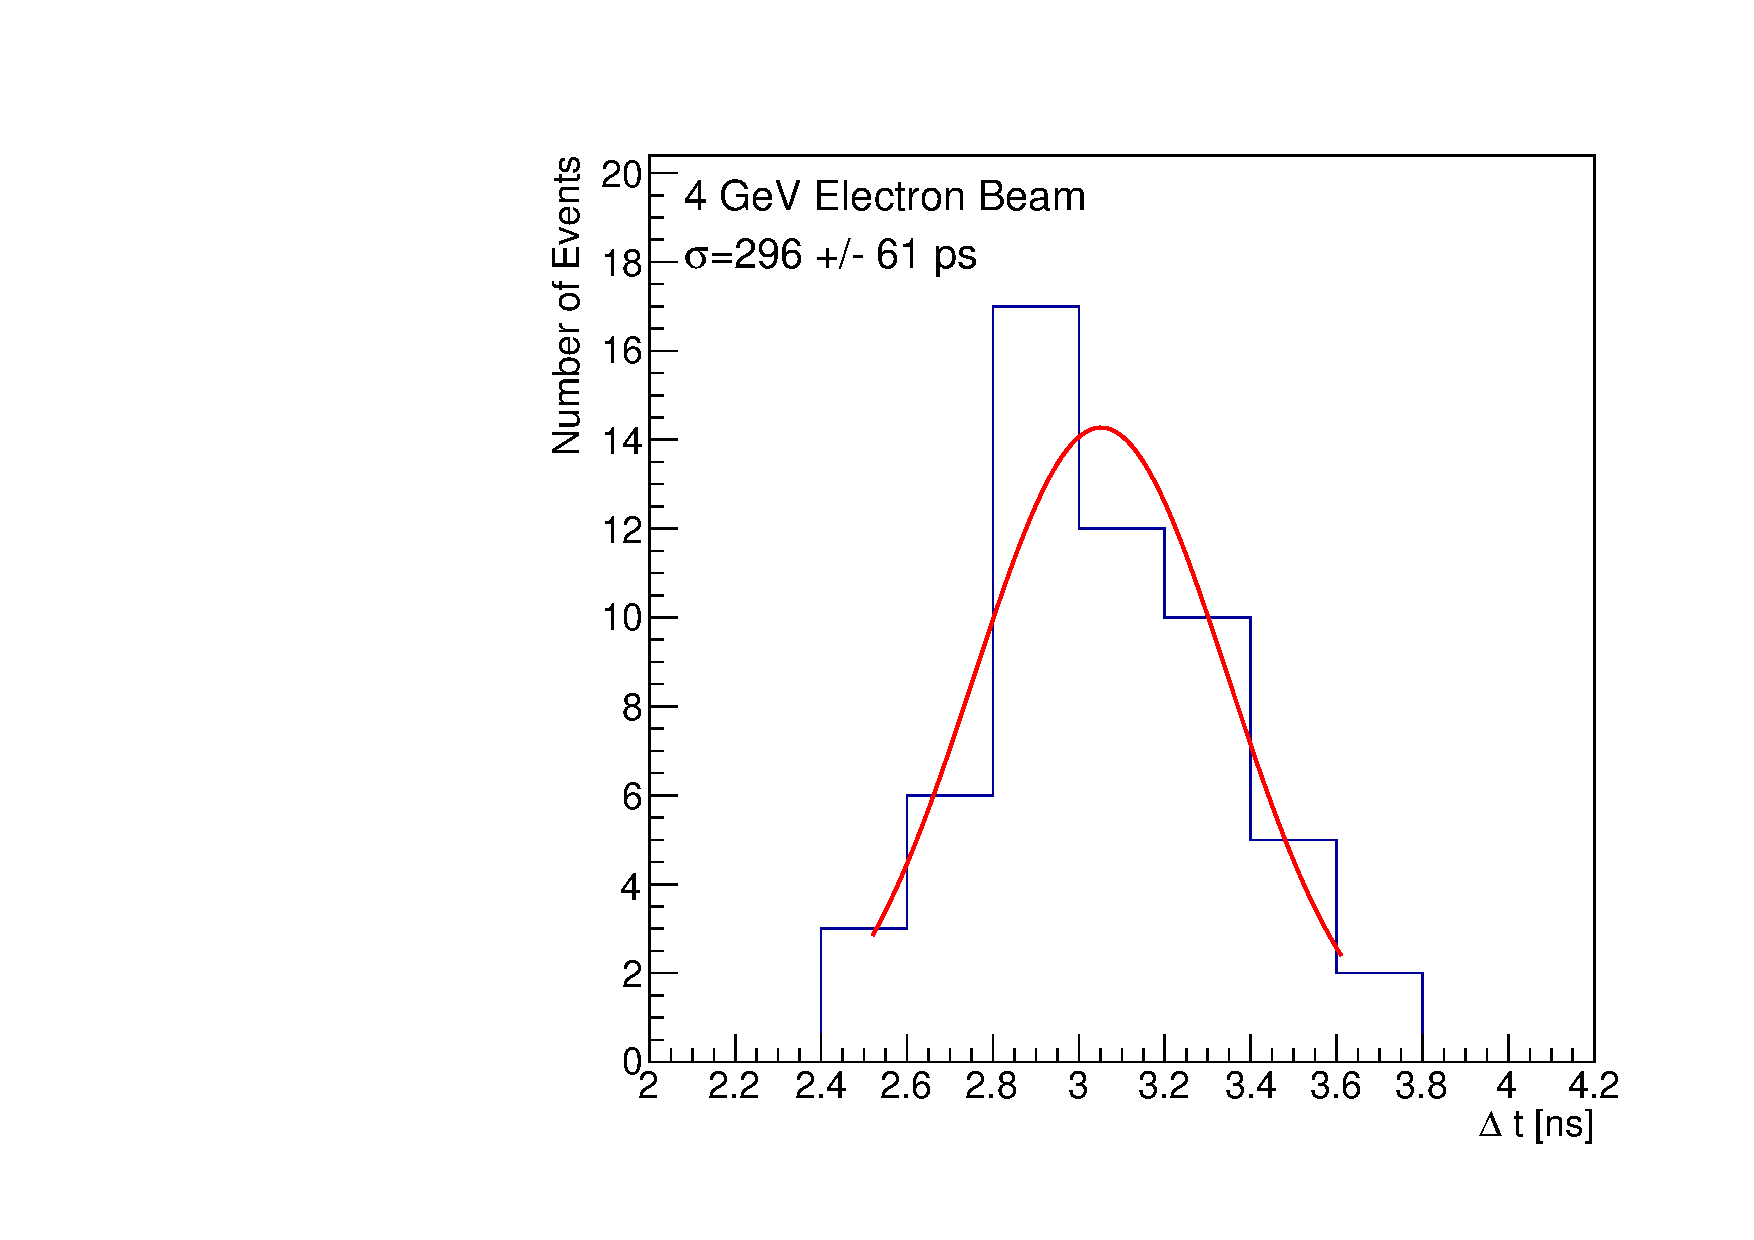
\includegraphics[width=0.23\textwidth]{figs/TOF_ShashlikDSB1Fiber_Electron_4GeV} 
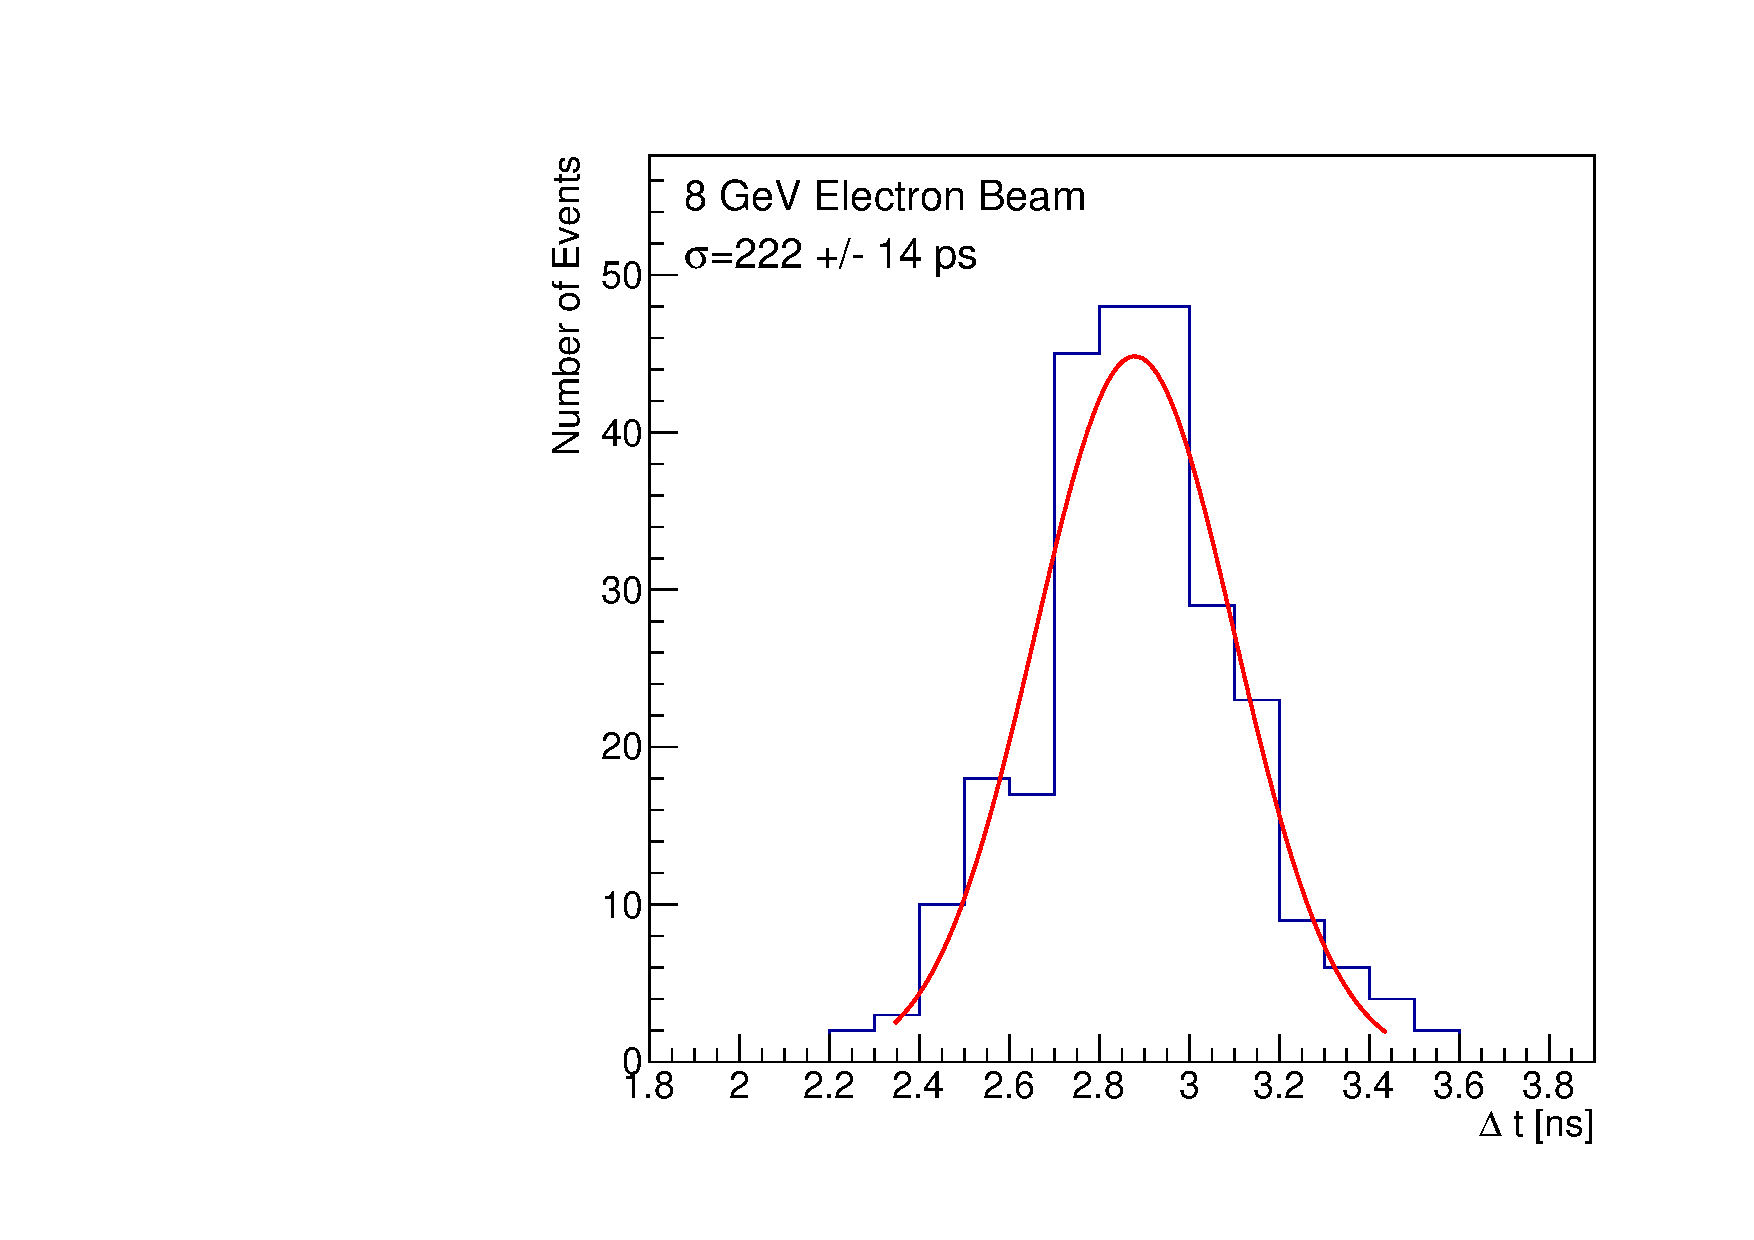
\includegraphics[width=0.23\textwidth]{figs/TOF_ShashlikDSB1Fiber_Electron_8GeV} 
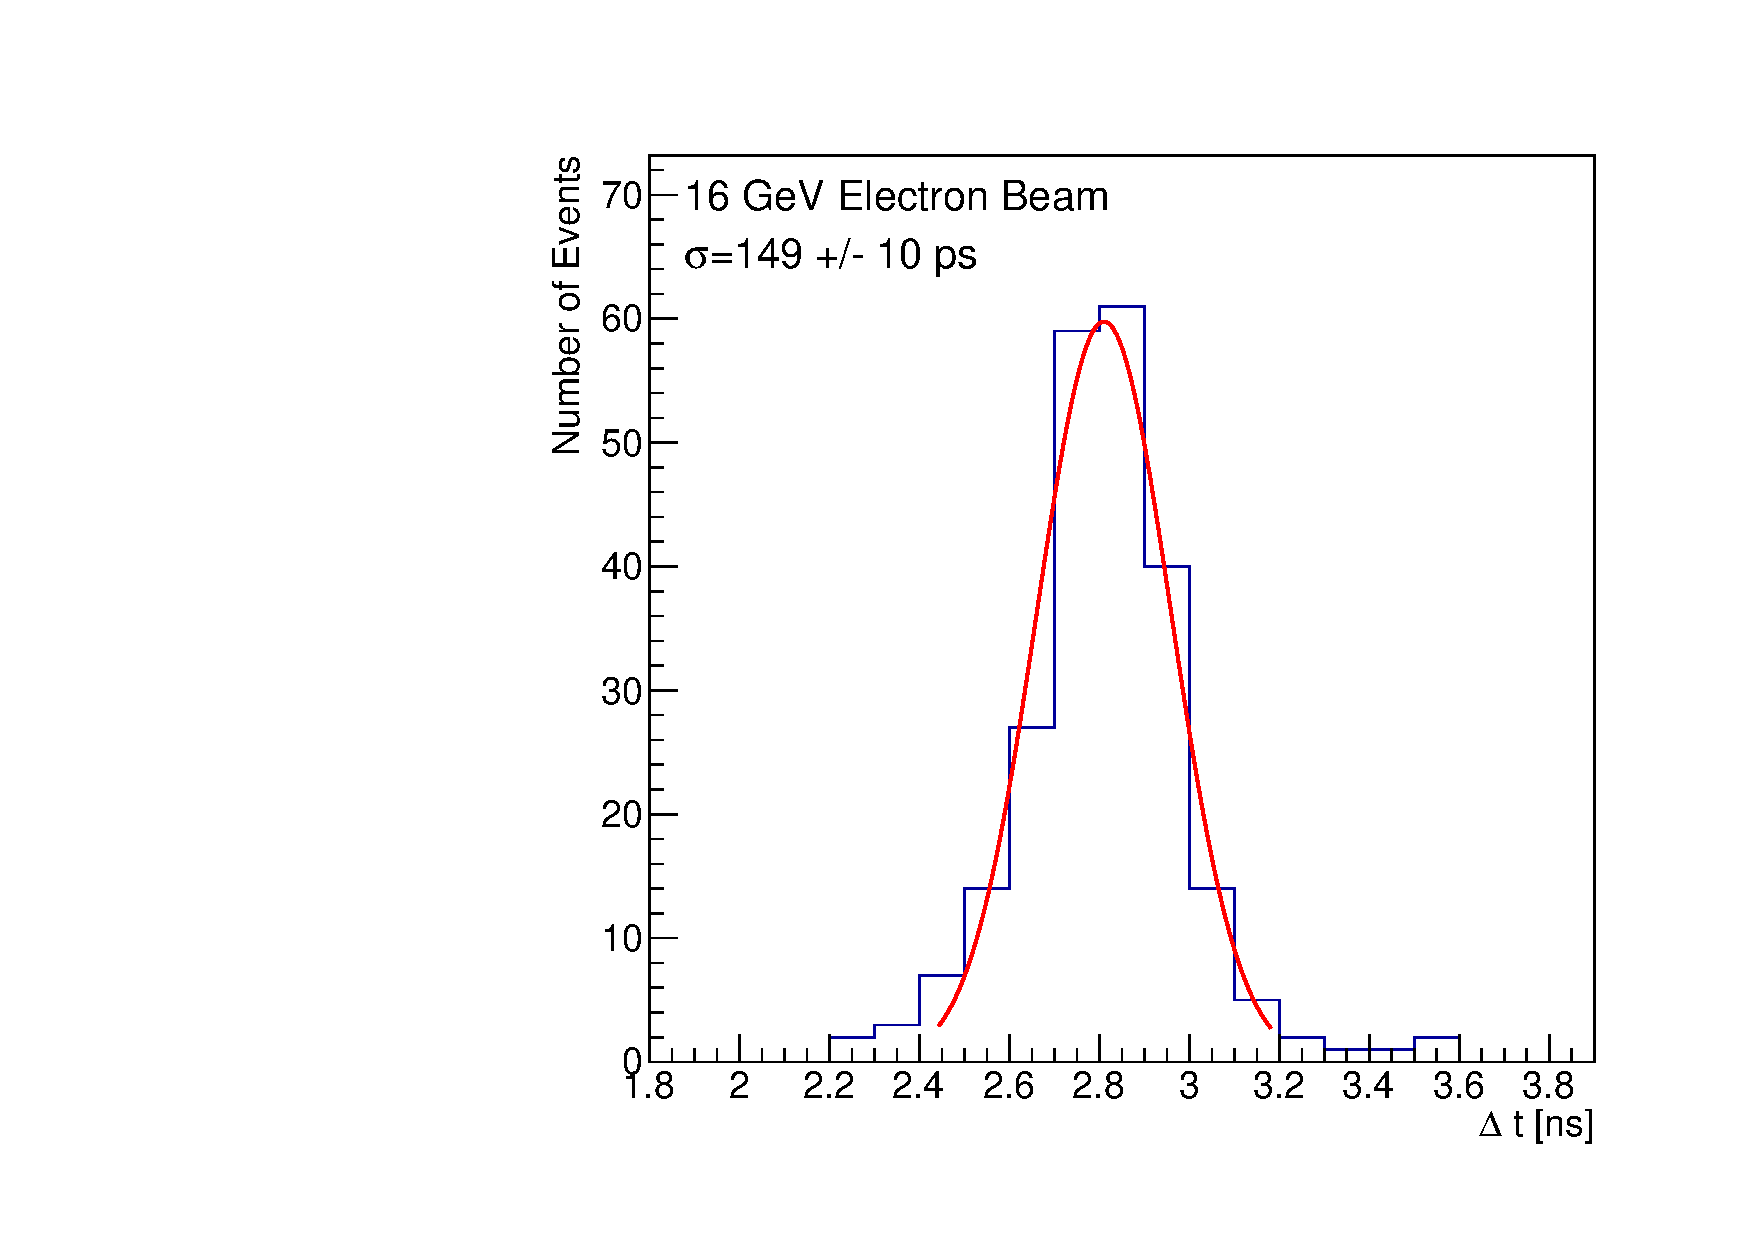
\includegraphics[width=0.23\textwidth]{figs/TOF_ShashlikDSB1Fiber_Electron_16GeV} 
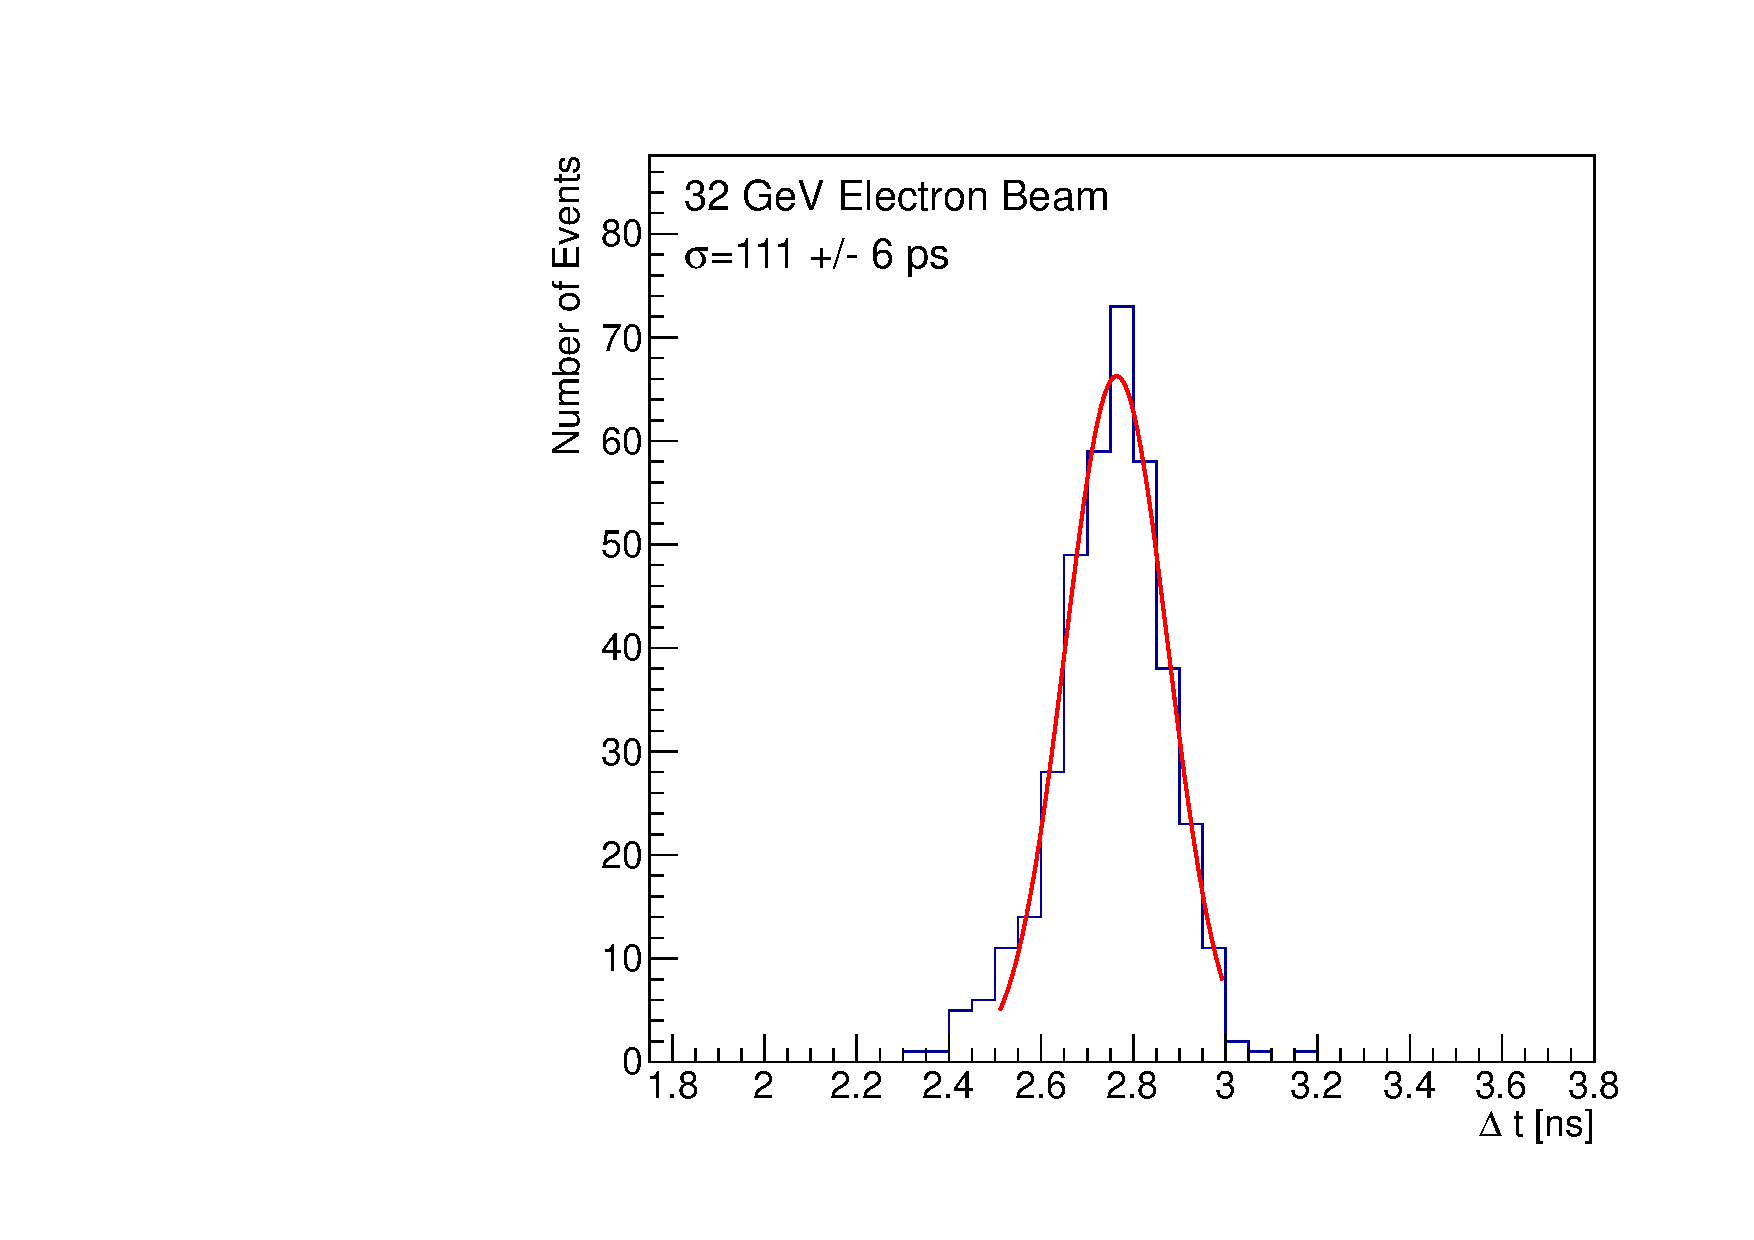
\includegraphics[width=0.23\textwidth]{figs/TOF_ShashlikDSB1Fiber_Electron_32GeV} 
\caption{\small Time of flight distributions for the LYSO-tungsten shashlik calorimeter
using DSB1 fibers for electron beams with varying beam energies.} 
\label{fig:ShashlikFiberTOF}
\end{figure}

\subsubsection{Directly coupled MCP-PMTs to LYSO shashlik plates}
In this setup the MCP-PMT photodetectors are directly coupled to the edges of two adjacent LYSO layers in the shashlik
calorimeter and scintillation light is directly transported to the photodetector
through the edges of the tile layers. A schematic diagram and corresponding
picture  of the experimental setup are shown in
Figure~\ref{fig:ShashlikSideReadoutSetup}. In
Figure~\ref{fig:ShashlikSideReadoutExposedLayersPhoto}, we show a zoomed-in
photograph of the exposed LYSO plates from which the scintillation light signal
is extracted.

\begin{figure}[ht!] \centering
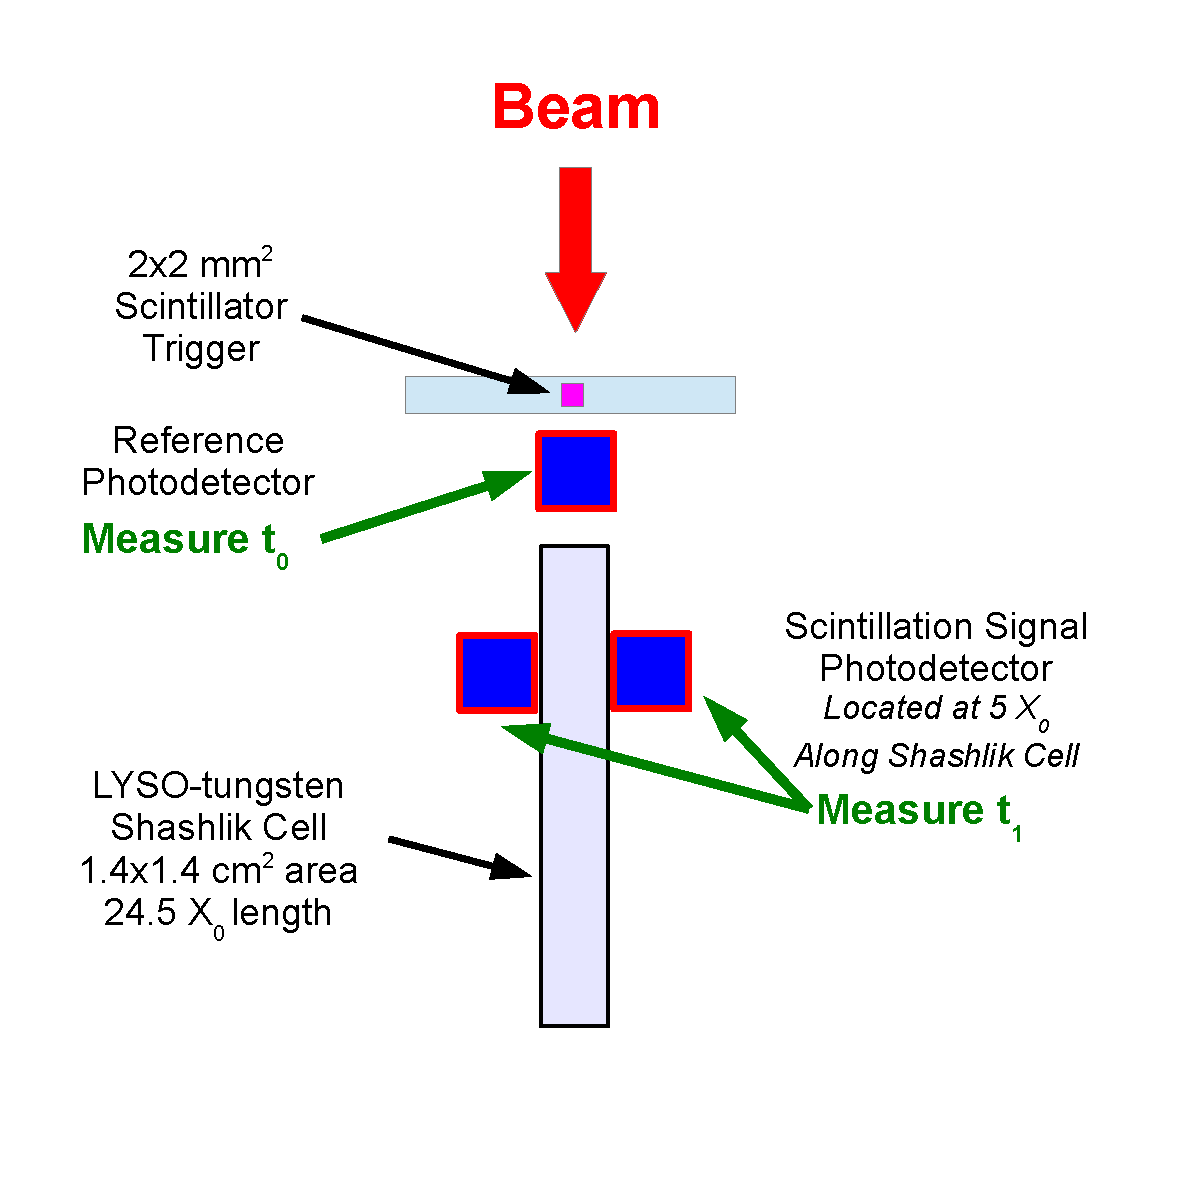
\includegraphics[width=0.45\textwidth]{figs/ShashlikSideReadoutSetupSchematic} 
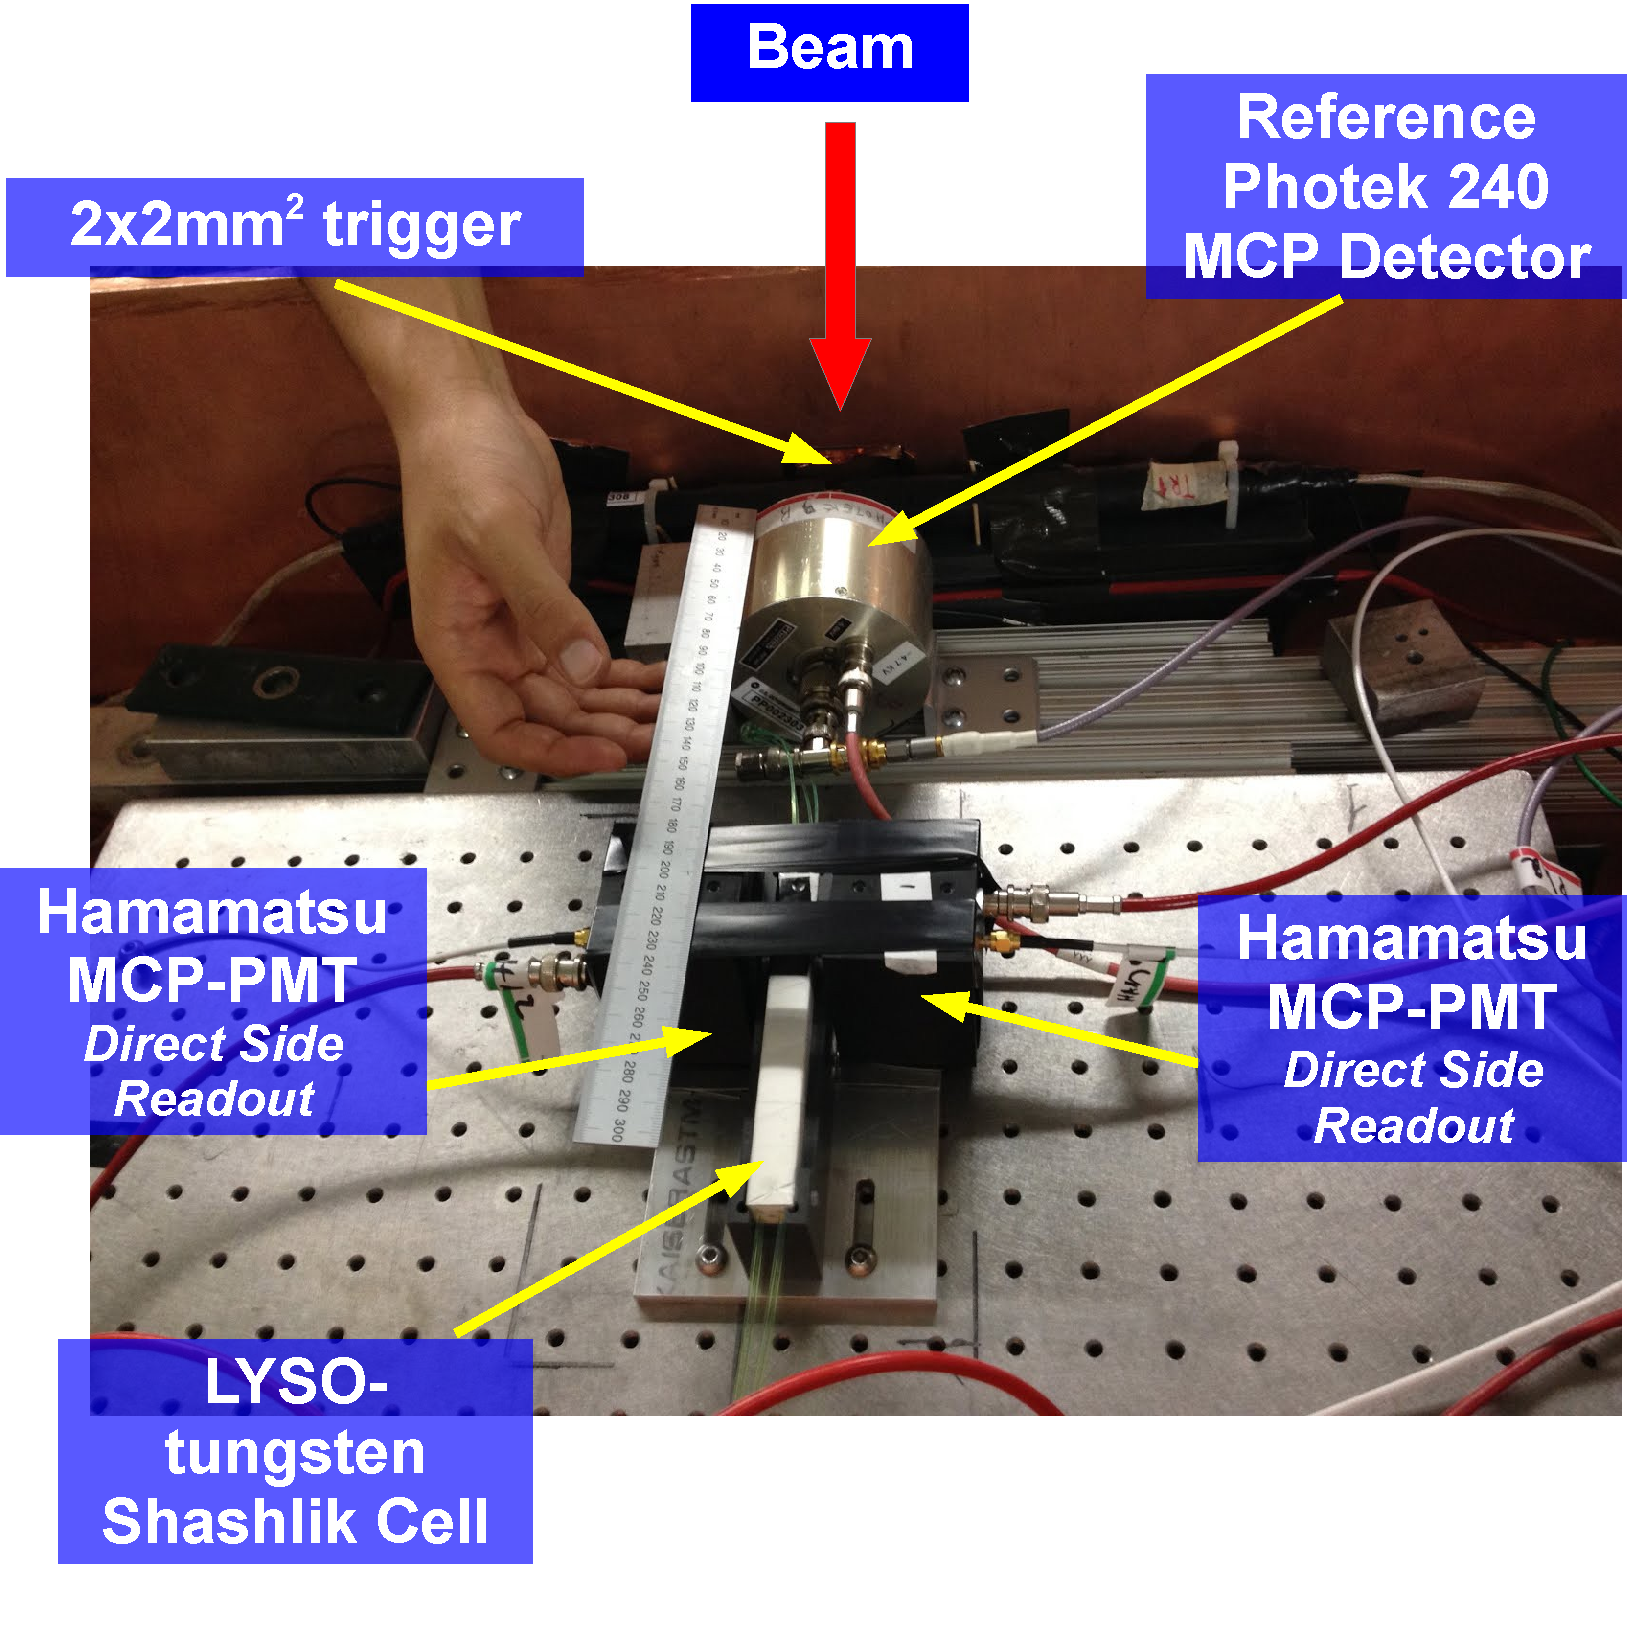
\includegraphics[width=0.45\textwidth]{figs/ShashlikSideReadoutPhotoB} 
\caption{ \small A schematic diagram of the experimental setup for the
time of flight measurement using the LYSO-tungsten shashlik calorimeter
with signal extraction from the edges of two LYSO plates, along
with a picture of the experimental setup. } 
\label{fig:ShashlikSideReadoutSetup}
\end{figure}

\begin{figure}[ht!] \centering
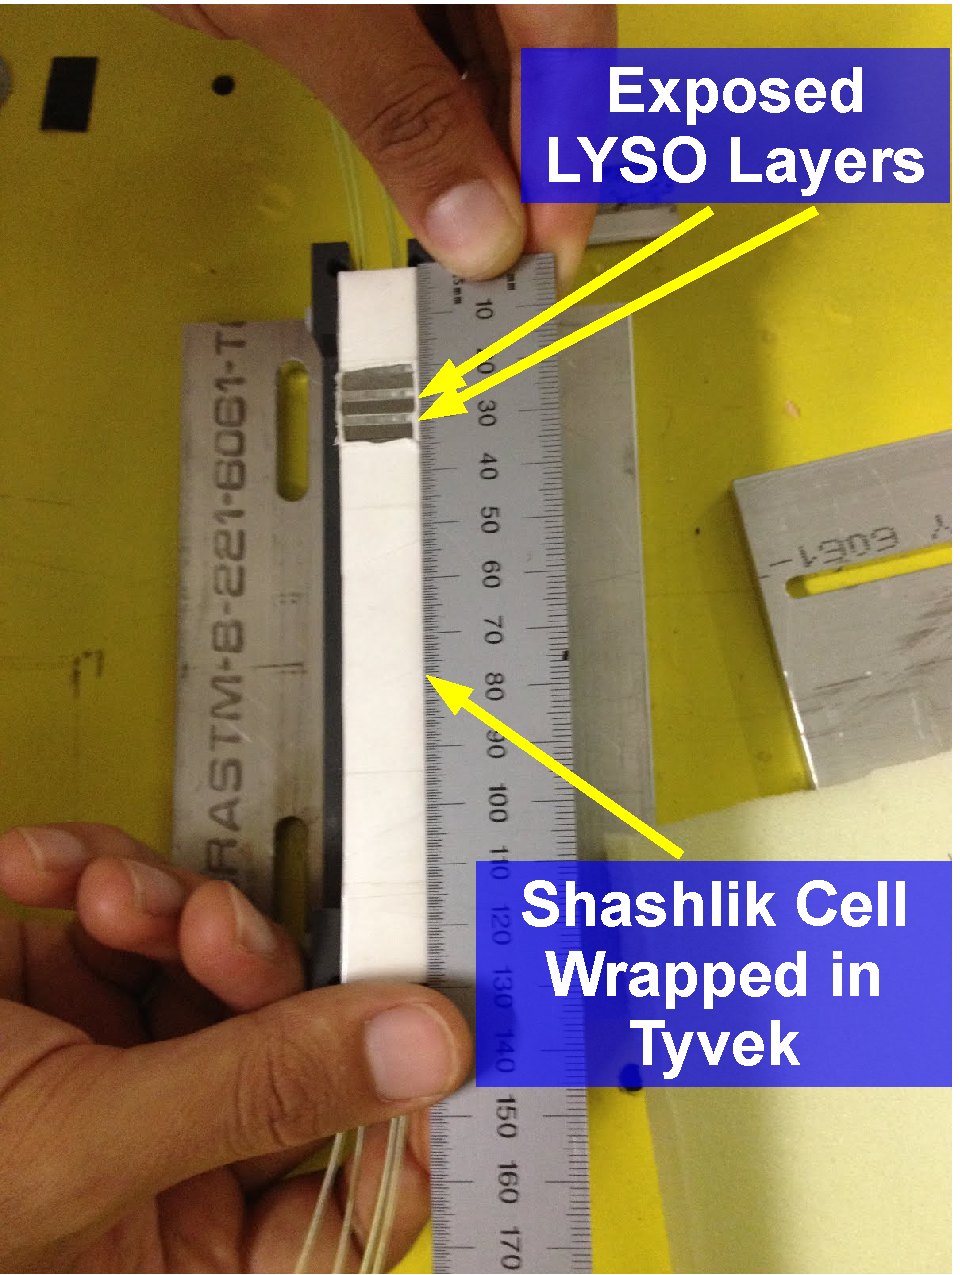
\includegraphics[width=0.30\textwidth]{figs/ShashlikSideReadoutPhotoA} 
\caption{\small A photograph of the two exposed LYSO layers in the shashlik cell.
The scintillation light signal is extracted by optically coupling
the edges of these two exposed LYSO layers to MCP-PMT
photodetectors. } 
\label{fig:ShashlikSideReadoutExposedLayersPhoto}
\end{figure}


With this setup we invoke an interplay between the light propagation jitter 
and the limited photostatistics. By placing the photodetectors in direct contact with the edges 
of two LYSO layers, we minimize the distance the scintillation light  travels to reach the 
photodetectors, and reduce the impact of light propagation jitter on the time measurement 
resolution. However in this setup we have also reduced the available photostatistics, as we collect 
light from only a small fraction of the shashlik cell. In Figure~\ref{fig:ShashlikSideReadoutTOF},
we show the time of flight distributions for electron beams at various energies,
fitted to gaussian functions. The width of the best-fit gaussian is plotted as a
function of the beam energy in Figure~\ref{fig:ShashlikSideReadoutTOFResolutionVsEnergy}. The 
best time resolution that we obtain is about $55$~ps, and fitting the result to the sum of
a $1/\sqrt{E}$ term and a constant term, we find a constant term of about
$30$~ps. 

\begin{figure}[ht!] \centering
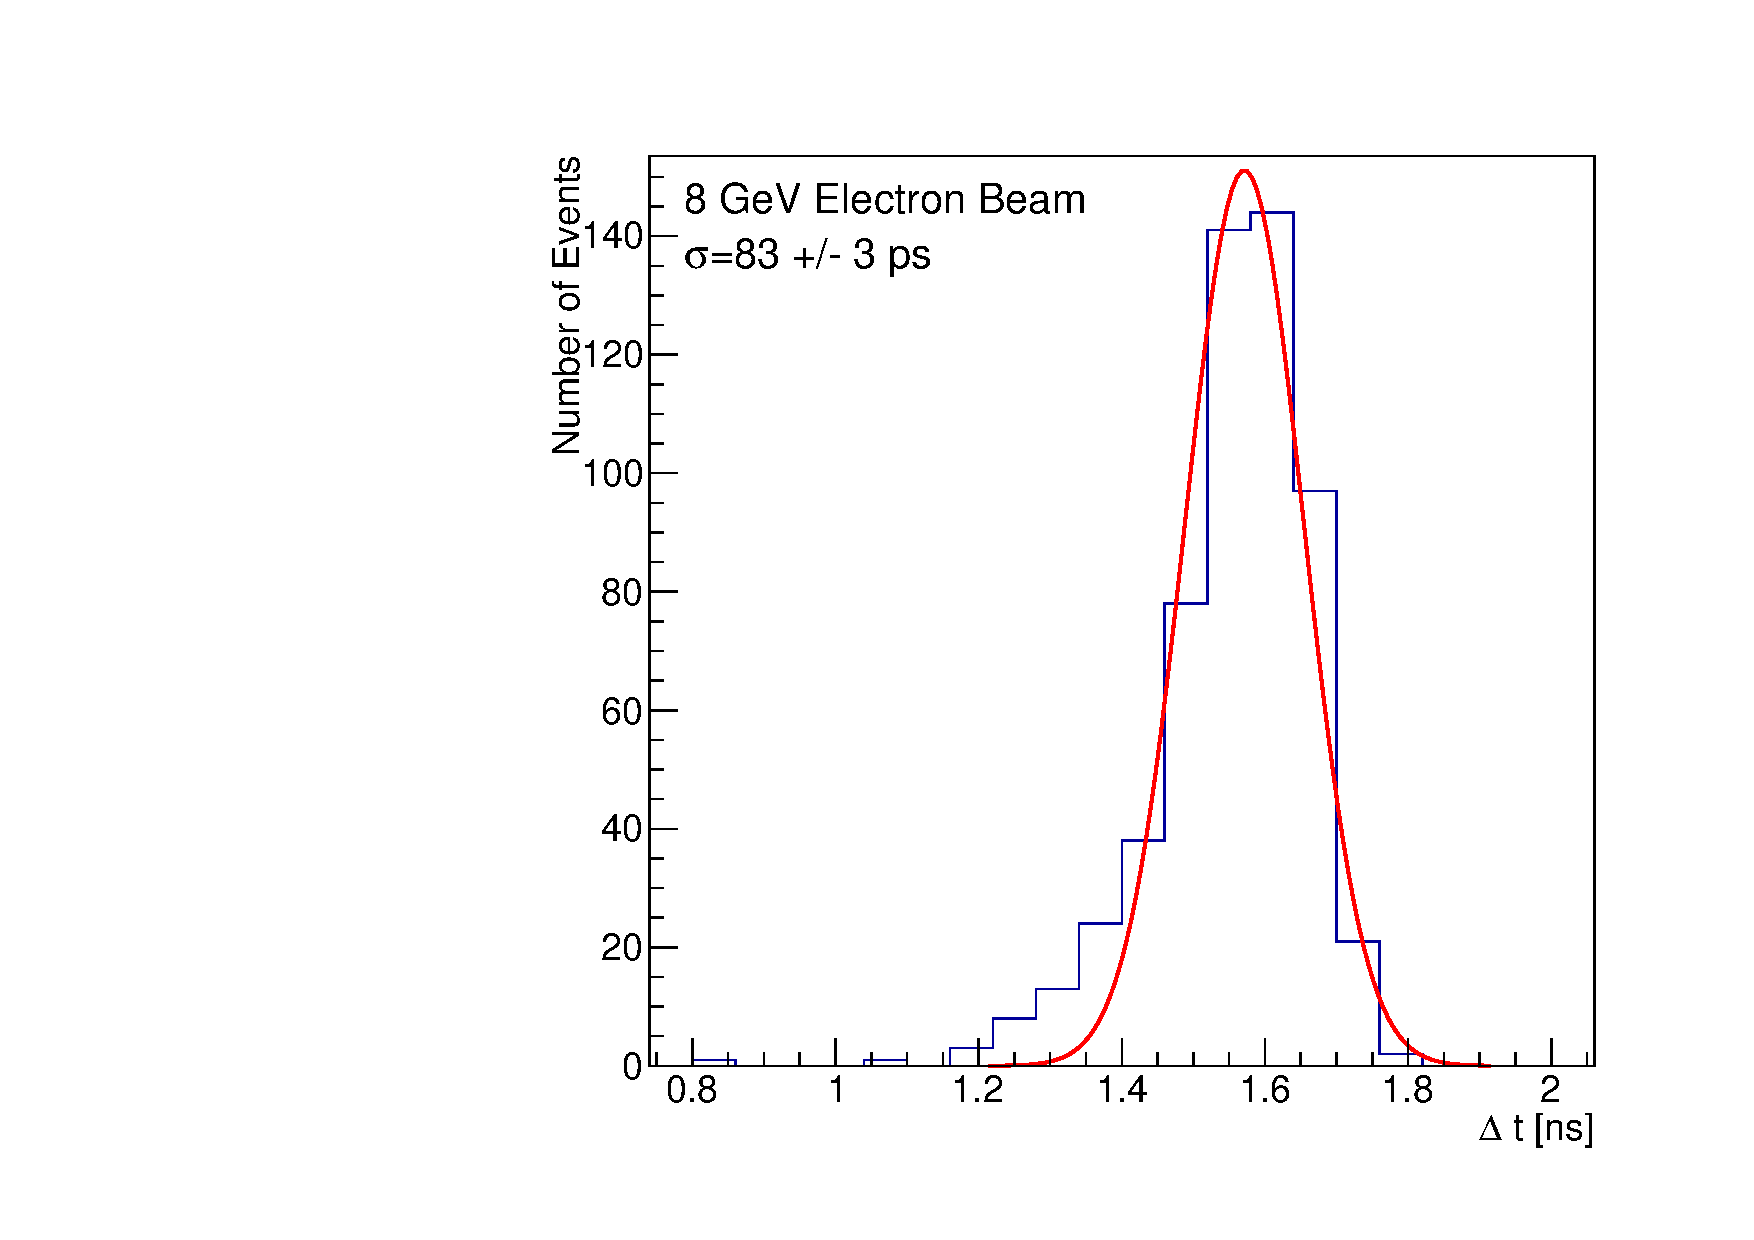
\includegraphics[width=0.32\textwidth]{figs/TOF_ShashlikSideReadout_Electron_8GeV} 
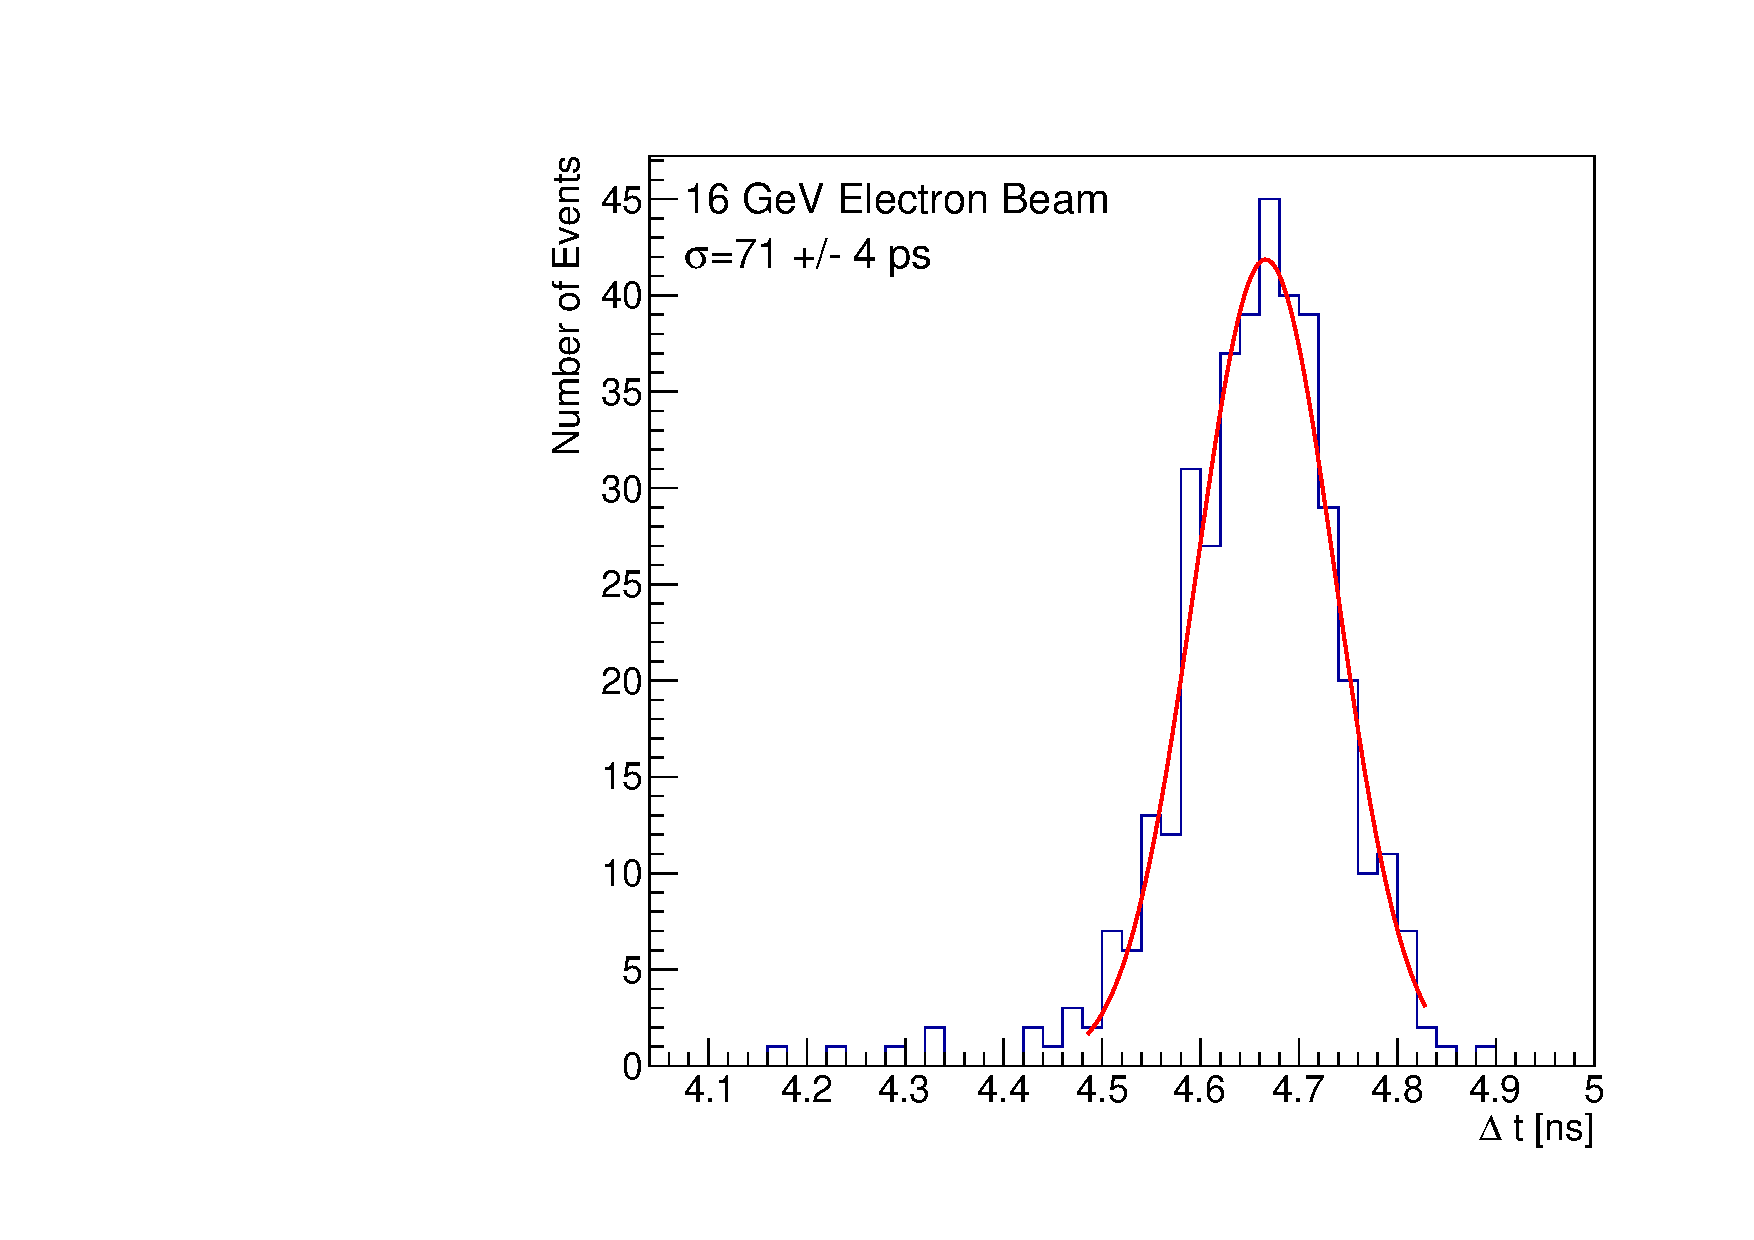
\includegraphics[width=0.32\textwidth]{figs/TOF_ShashlikSideReadout_Electron_16GeV} 
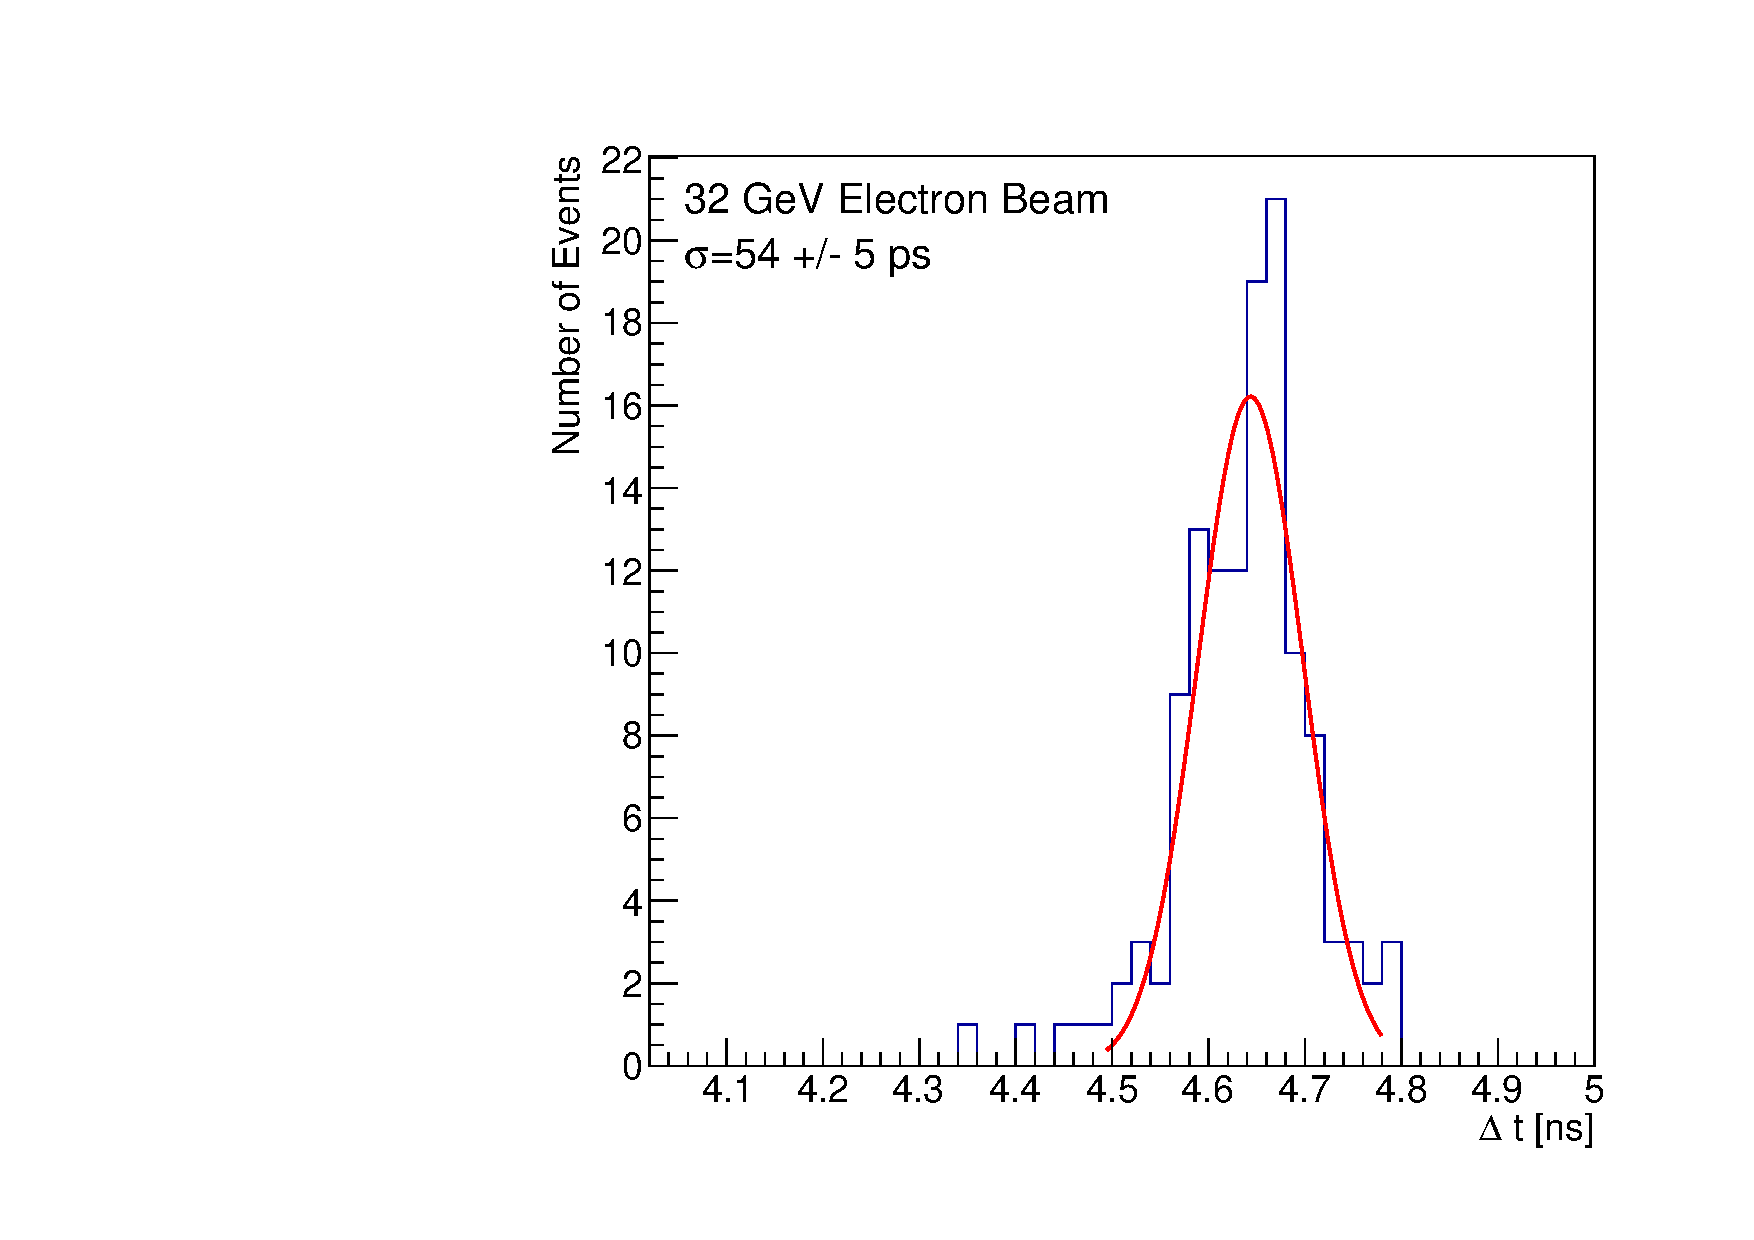
\includegraphics[width=0.32\textwidth]{figs/TOF_ShashlikSideReadout_Electron_32GeV} 
\caption{ Time of flight distributions for the LYSO-tungsten shashlik calorimeter
with signal extracted from the edges of two LYSO layers. } 
\label{fig:ShashlikSideReadoutTOF}
\end{figure}


\begin{figure}[h] \centering
\caption{\small}
\label{fig:LYSOCubeTOFResolutionVsEnergy}
\end{figure}
\begin{figure}[ht!] \centering
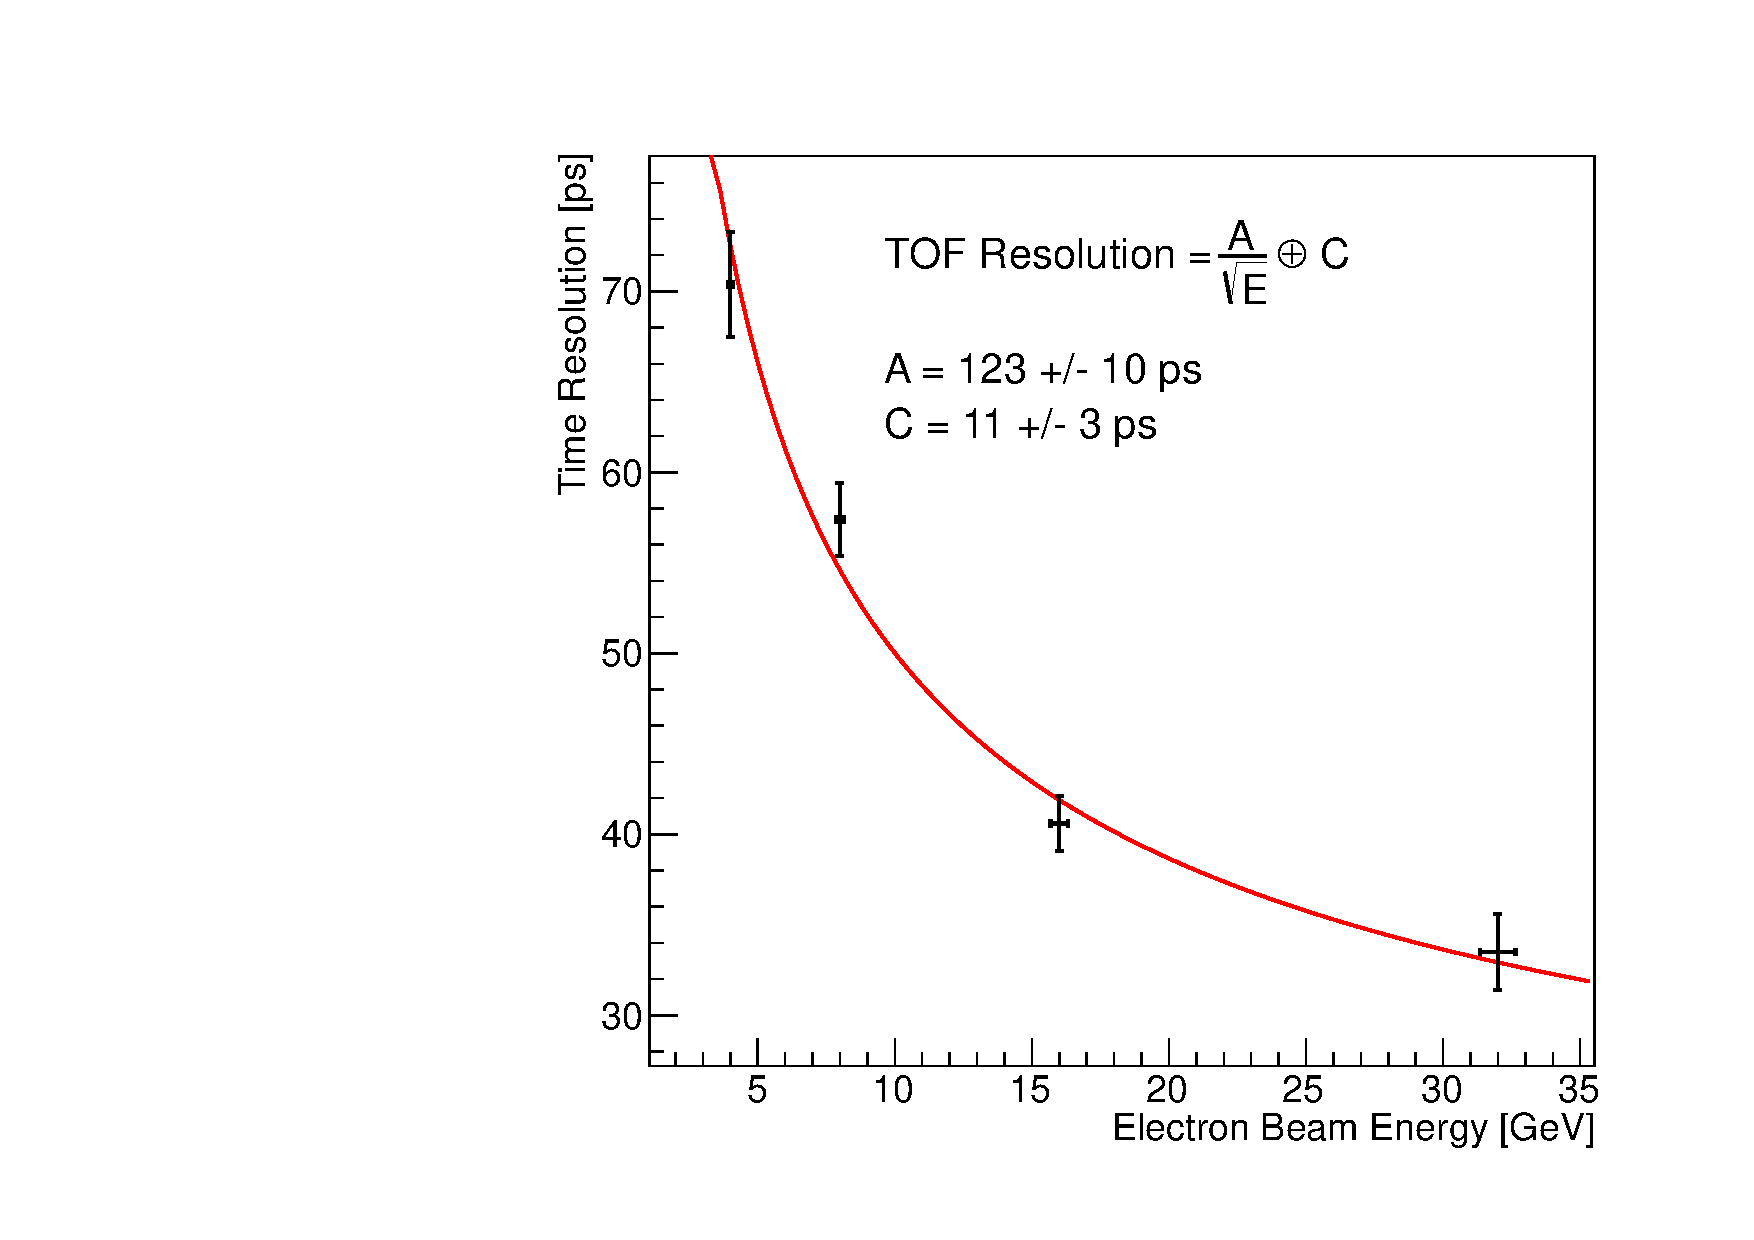
\includegraphics[width=0.32\textwidth]{figs/TimeResolutionVsEnergy_CrystalCube} 
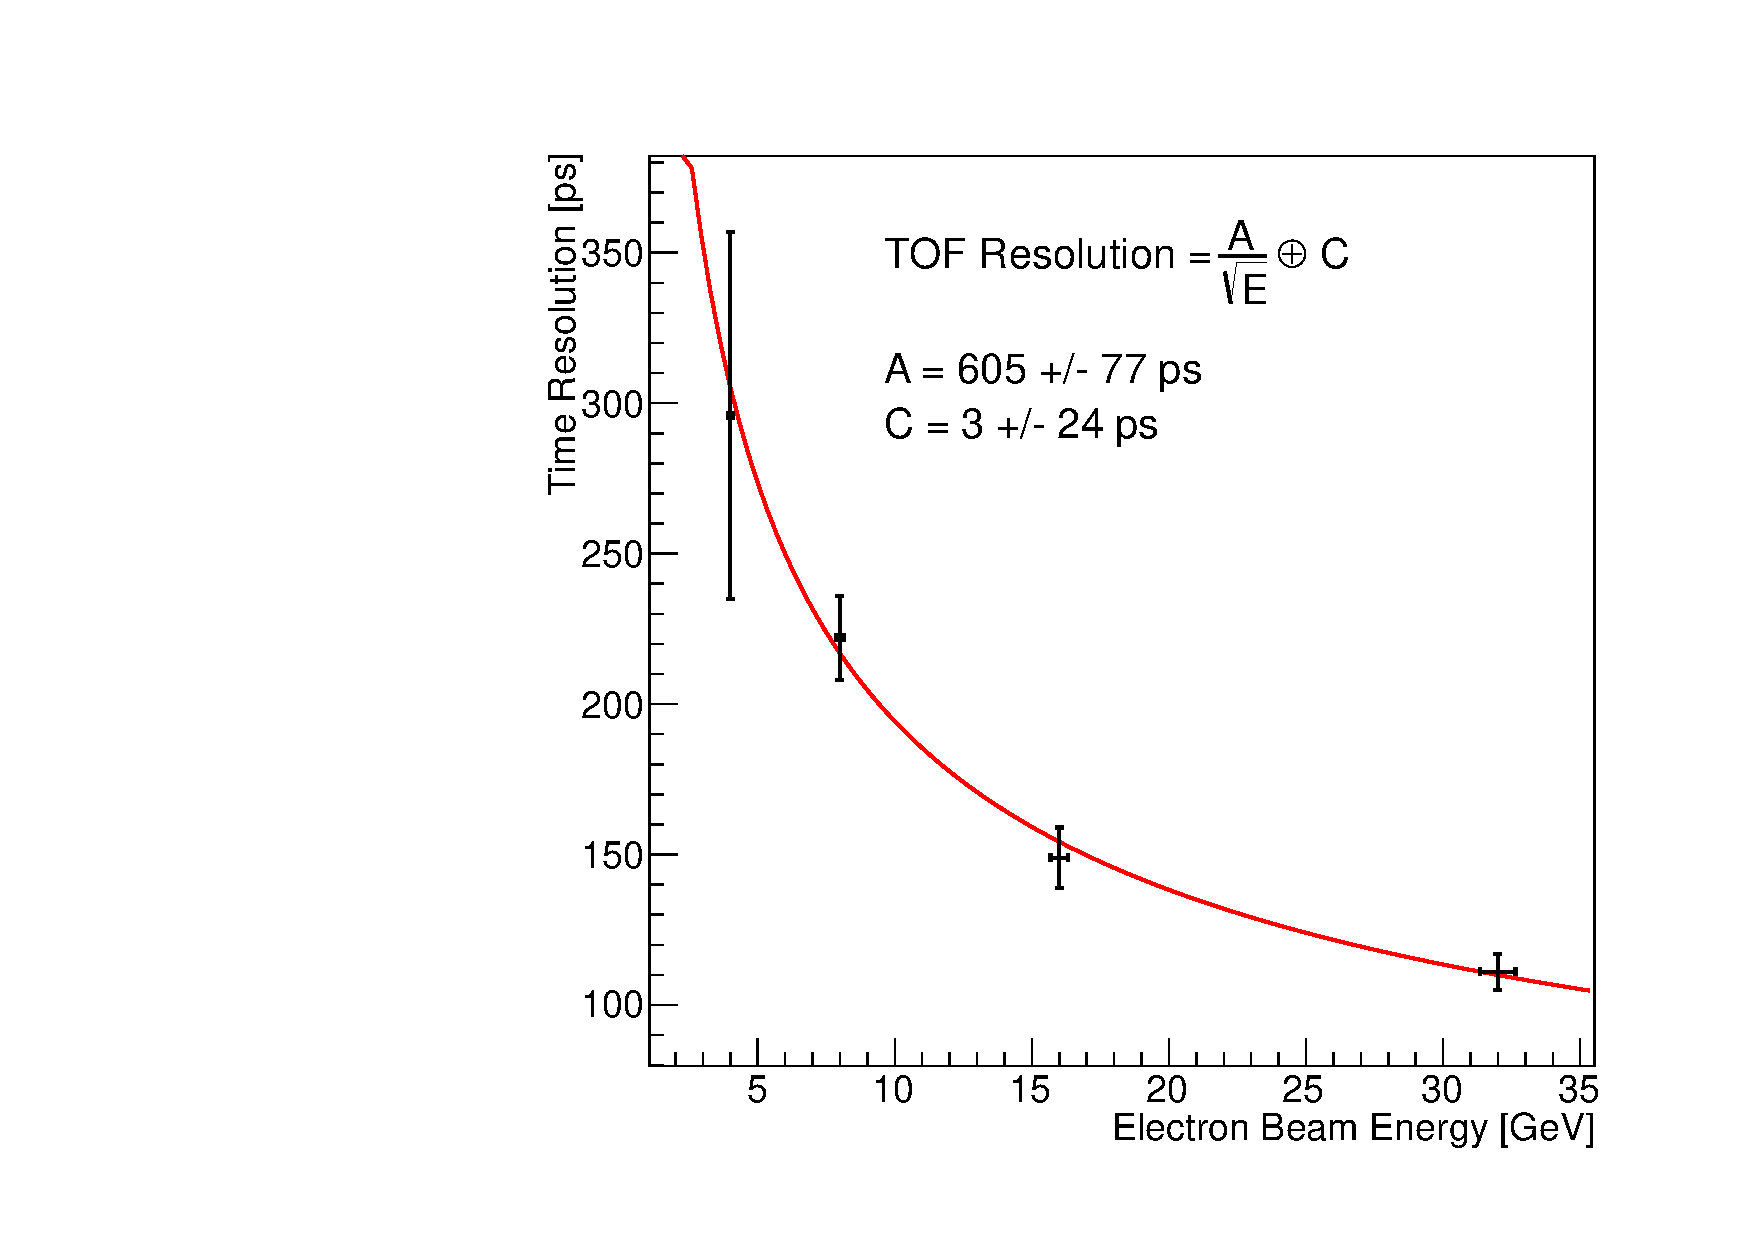
\includegraphics[width=0.32\textwidth]{figs/TimeResolutionVsEnergy_ShashlikDSB1Fiber} 
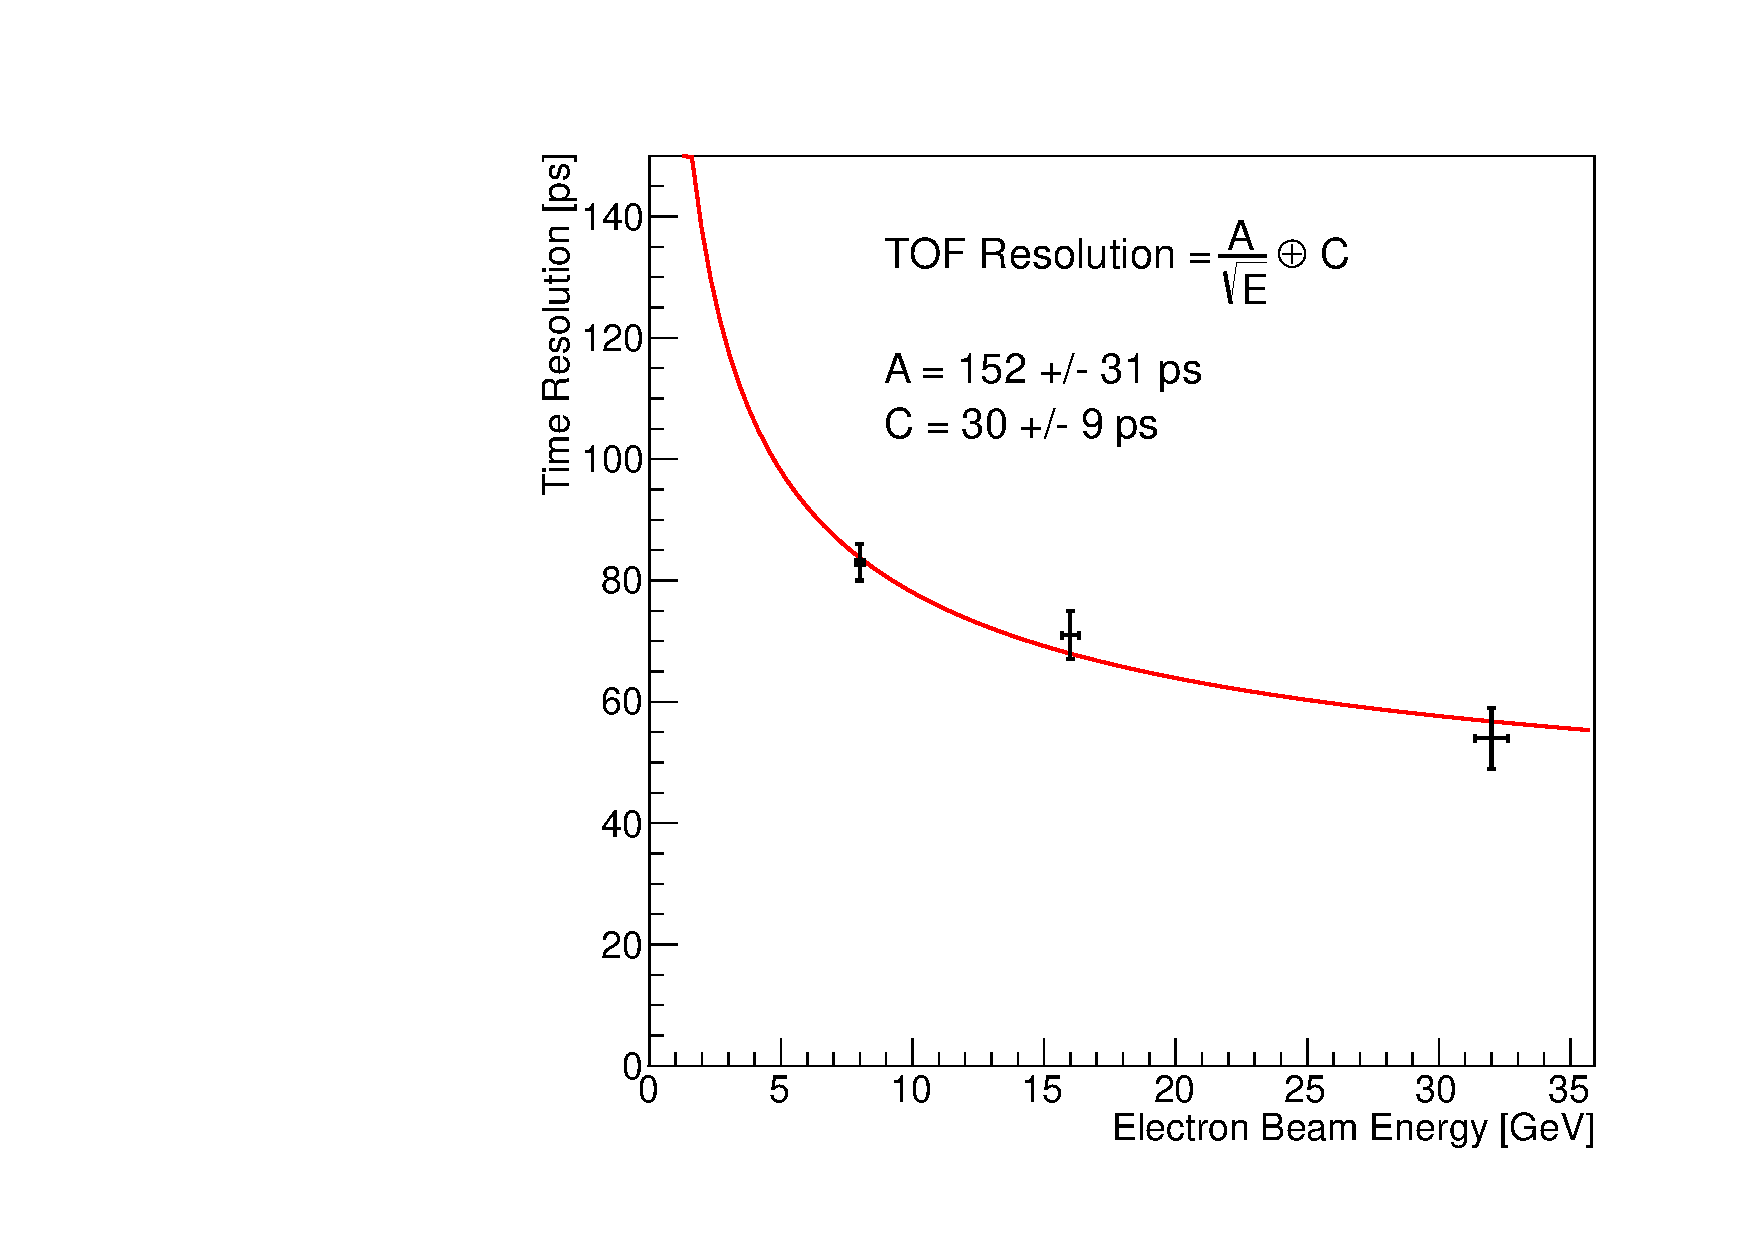
\includegraphics[width=0.32\textwidth]{figs/TimeResolutionVsEnergy_ShashlikSideReadout} 
\caption{ Timing resolution measurement as a function of the electron beam energy for (left) the LYSO cube
sampling calorimeter  
%Note that the energy absorbed in the LYSO cube is a small fraction of the incident electron energy. (Middle)The time resolution measured using  
(middle) the LYSO-tungsten shashlik
calorimeter read-out with  DSB1 fibers %is plotted as a function of
%the electron beam energy, and fitted to a $1/\sqrt{E}$ functional form. 
(right)  the LYSO-tungsten shashlik calorimeter read-out directly by optically coupling to the edges of two LYSO layers. 
%is plotted as a function of the electron beam energy, and fitted to the sum 
In all cases we fit the data with a function of $1/\sqrt{E}$  and a constant term. }
\label{fig:ShashlikSideReadoutTOFResolutionVsEnergy}
\end{figure}

In summary, we find that removing the impact of the wavelength shifting
mechanism and minimizing the impact of optical transit does indeed improve the
time resolution, but at a cost in photostatistics. Results obtained in this
experiment suggest that a LYSO-tungsten shashlik calorimeter with edge readout
can likely achieve $30$~ps resolution provided some improvement to the light
collection efficiency is achieved.

\section{Results Discussion and Summary }
This section described studies characterizing the timing performance
of LYSO-based calorimeters. Using a (1.7~cm)$^{3}$ LYSO crystal that
samples the electromagnetic showers created by electrons of various energies
ranging from $4$~GeV to $32$~GeV at about $4.5$~$X_{0}$, we infer that the
contribution to the time resolution from event-by-event fluctuations of the
shower profile, the scintillation process, and the light propagation is less than
$30$~ps. Studies using different wavelength shifting fibers in a LYSO-tungsten shashlik calorimeter 
demonstrates that the choice of the fiber affects the timing performance. Besides the absorption 
and re-emission processes in the fibers, we found that another important factor influencing
the timing performance is the light extraction efficiency. Using DSB1 fibers, despite being 
photostatistics limited, we obtained a best time resolution of about $100$~ps.  A future 
development of such a detector will  be focused on increasing the light collection efficiency.
In a setup where  the scintillation light from the LYSO-tungsten
shashlik calorimeter is extracted via the edges of two LYSO layers, thereby
removing completely the wavelength shifting mechanism and long light propagation distance, 
we achieve a best time resolution of $55$~ps. The result  indicates  that such a
calorimeter design can achieve the $30$~ps time resolution benchmark obtained with the LYSO cube
provided some improvement to the light collection efficiency. 

In comparing results using different light extraction schemes, we find that at a
given light yield the time resolution depends significantly on the light
propagation fluctuations. As the light yield increases the dependence on the
light propagation fluctuations is reduced. The effect can be seen in the summary
Figure~\ref{fig:ShashlikFiberAndCubeTOF} where we show the dependence of the
time resolution on the average pulse height for the shashlik cell with light
extracted through the DSB1 fibers and for the sampling calorimeter with the LYSO
cube. For the same average pulse height of 500 mV, the LYSO cube time resolution
is about half of the shashlik using the DSB1 fibers which have also twice the
rise time. As the pulse height increases the time resolution improves.
Extrapolating to the regime of very large light yield, we should be able to
reach asymptotically the best resolution without limitations from the light
propagation fluctuations. 


\begin{figure}[ht!] \centering
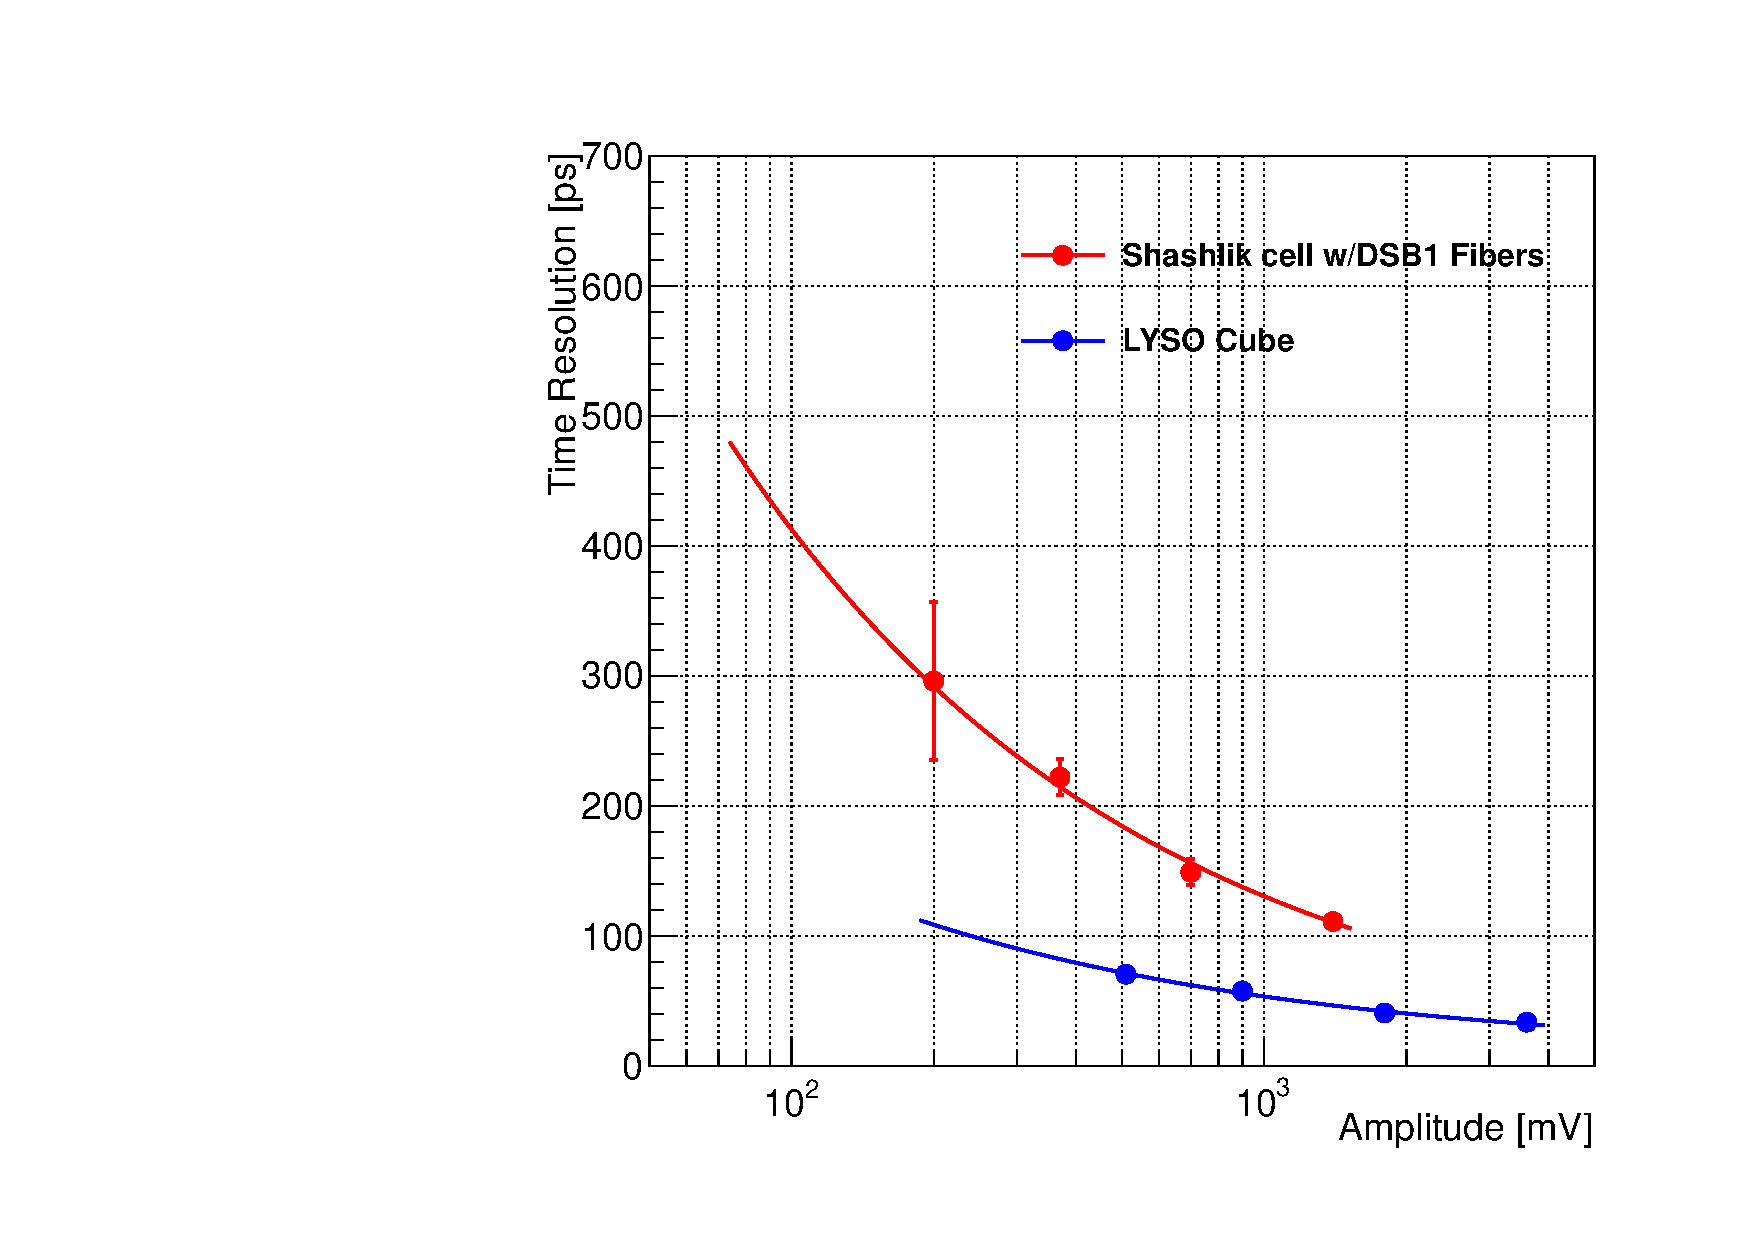
\includegraphics[width=0.55\textwidth]{figs/TimeResolutionVsEnergy_ShashlikDSB1FiberAndCube} 
\caption{\small Comparison of time resolutions obtained with the $(1.7$~cm$)^{3}$ LYSO cube (blue), 
and the LYSO-tungsten shashlik calorimeter with light extracted using DSB1 fibers (red). 
 The x-axis in this figure displays the amplitude of the
signal, corrected for the attenuation factors. }
\label{fig:ShashlikFiberAndCubeTOF}
\end{figure}

In summary, using a LYSO-based calorimeter and different light propagation experimental setups 
we obtain about $30$~ps resolution time measurement for the maximum light yield achieved. 
As a follow-up we will investigate the time resolution in the limit of very large light yield, 
and attempt to improve the light collection efficiency in these types of detectors.

\section{Acknowledgements} 
I would like to thank Erik Ramberg and Sergey Los for their help and support of this work, and Aria Soha and the FTBF test beam facility for
the beam delivery and control. We thank Randy Ruchti for providing us with
the DSB1 fibers used in the measurements, and Eileen Hahn for the high quality
work in polishing the fibers. We would also like to thank Ewa Skup and Geoff Savage for help with
operation of the Cherenkov counters, and to Todd Nobel for organizing and providing
supporting equipment at FTBF.

This work is supported by funding from Fermi Research Alliance, LLC under Contract No. DE-AC02-07CH11359 with the United States Department of Energy and from California Institute of Technology High Energy Physics under Contract DE-SC0011925 with the United States Department of Energy. 

\clearpage
\chapter{MCP-BASED Calorimeters}\label{mcp-cal}
In this chapter another precision timing calorimetric propototype using micro-channel plates (MCP)  as the
sensitive medium is studied.

\section{Introduction}
The use of micro-channel plates (MCP) as the sensitive element of a shower-maximum
detector or a calorimeter has been studied in the
past~\cite{Derevshchikov:1990ej,Albayrak-Yetkin:2013xga}. These studies
demonstrated the linearity in the multiplicity of secondary shower particles
that have energies that the MCP can detect. Such detectors are also a promising
option for achieving time measurement precision at the level of a few tens of
picoseconds~\cite{MCPFastCaloNIMA,Ronzhin:2015pba,Ronzhin2015288,Brianza2015216}.
Moreover, such devices are intrinsically radiation hard and thus would tolerate
the harsh radiation environment at future hadron colliders, particularly when
operated without the reliance on a photocathode. In
reference~\cite{Ronzhin2015288}, it has been demonstrated that the intrinsic
fluctuations of electromagnetic showers induce jitter on the time measurement
that is less than $10$~ps, removing one important potential fundamental
limitation. A further advantage of MCPs is their capability for highly
segmented readout, allowing for the possibility of a highly granular calorimeter
with sub-millimeter spatial resolution. Such high-granularity calorimeters have
been studied in the context of detector concepts for the
ILC~\cite{Grondin:2010fe} and the HL-LHC upgrade of the CMS
experiment~\cite{Butler:2020886}, indicating that such calorimeters have
promising potential for substantial improvement in physics reach at the TeV
scale. The results in this chapter complement past
results~\cite{Anderson:2015gha,MCPFastCaloNIMA,Ronzhin:2015pba,Ronzhin2015288}
with additional studies of the position and time resolution for a calorimeter
prototype with highly granular readout.

The studies in this chapter use three different MCP-PMTs:
\begin{itemize}
\item Photek 240: the most performant device, which provides the best
      time resolution, and excellent uniformity across the detector. The main parameters
      of the Photek 240 were reported in Ref.~\cite{MCPFastCaloNIMA}. The pore
      size is 10~$\mu$m and the distance from the photocathode to the first
      amplification stage is 5.3~mm. The Photek 240 has a 41~mm$^2$ circular
      sensitive area, and it was operated 4.8~kV high voltage (HV). The gain at
      this voltage is about 10$^6$. The non-uniformity of the time response of the signal 
      is limited to below 3.9~ps across the full sensitive area.
\item Photonis XP85011: the anode of this MCP is composed of 64 pads, arranged
      as an $8\times8$ matrix. The size of each pad is $6\times6$~$\mathrm{mm}^{2}$. 
      The pore size is 25 $\mu$m. The non-uniformity  of the time response across the photocathode
      is $37$~ps~\cite{MCPFastCaloNIMA, Ronzhin2015288}. The HV applied to the Photonis XP85011 
      was 2.4~kV, with a corresponding gain of $10^6$. 
\item Photonis XP85012: mostly identical to XP85011, also composed of 64 pixels arranged as
      an $8\times8$ matrix. Additionally it can be operated in a mode with a reverse voltage applied 
      to photocathode, which enables us to effectively turn off any signals from 
      the photocathode. When operated in this mode, the only signals are 
      directly from secondary shower particles~\cite{Ronzhin:2015pba}.  
\end{itemize}

This chapter reports on the studies of the high-granularity shower-maximum detector prototype 
that uses the Photonis XP85011 MCP as the active element. As demonstrated in 
reference~\cite{MCPFastCaloNIMA}, due to the fact that the input window is very thin, the signal in this device is dominated by direct detection of secondary shower particles, 
while Cherenkov photon signals contribute only $30\%$ of the amplitude.
The MCP is used to sample the electromagnetic shower induced by a beam
of electrons impinging into a tungsten absorber layer that has a thickness of about 4 radiation lengths ($X_{0}$). The
MCP-PMT is read out with a pixelated anode, with square pixels of size 
$6\times6$~$\mathrm{mm}^{2}$. The energy of the electromagnetic showers is reconstructed 
using the total collected charge and the positions are reconstructed using a simple
energy-weighting algorithm, described in Section~\ref{sec:position}.
Through the use of a high-precision motorized stage, a position scan is
performed during beam-tests and the position resolution of the shower-maximum
detector is obtained. Finally, the precision of measuring the
arrival time of electromagnetic showers with such a pixellated shower-maximum
detector is investigated.

This chapter is organized as follows. Section~\ref{sec:setup} gives a
description of the
experimental setup,
Section~\ref{sec:reconstruction} presents the event selection and pulse
reconstruction, Section~\ref{sec:position} and~\ref{sec:timing} the
presents the results on position measurements and timing resolutions, respectively. 

\section{Experimental Setup} \label{sec:setup} The experiment was performed at
the MTEST location of the Fermilab Test Beam Facility using an $8$~GeV beam
primarily comprised of electrons. A differential Cherenkov counter, located
further upstream of the MTEST location, was used to enhance the purity of
electrons and to suppress pions, by requiring a signal consistent with a passage
of electrons through the device. All other detectors were placed inside a dark
box lined with copper foil for electromagnetic shielding. A photograph of the
experimental setup within the dark box is shown in Figure~\ref{fig:setup}. A
scintillator of size $1.7$~mm$\times$~$2.0$~mm optically coupled to two
photomultiplier tubes, one on each side, was used to trigger the data
acquisition and to constrain the trajectory of the electrons from the beam.
Downstream of the trigger, a tungsten absorber with a thickness of about $1$~cm,
equivalent to about 4 radiation lengths, was placed. The Photonis XP85011
MCP-PMT with pixelated readout was set on a high precision motorized stage and
placed behind the tungsten absorber. The precision of the motorized stage is
about $0.1$~mm. To avoid unintended early showers due to interactions with the
material of the casing and MCP device, the Photek 240 MCP-PMT was placed behind
the Photonis XP85011 MCP-PMT. 

\begin{figure}[htbp] 
\centering
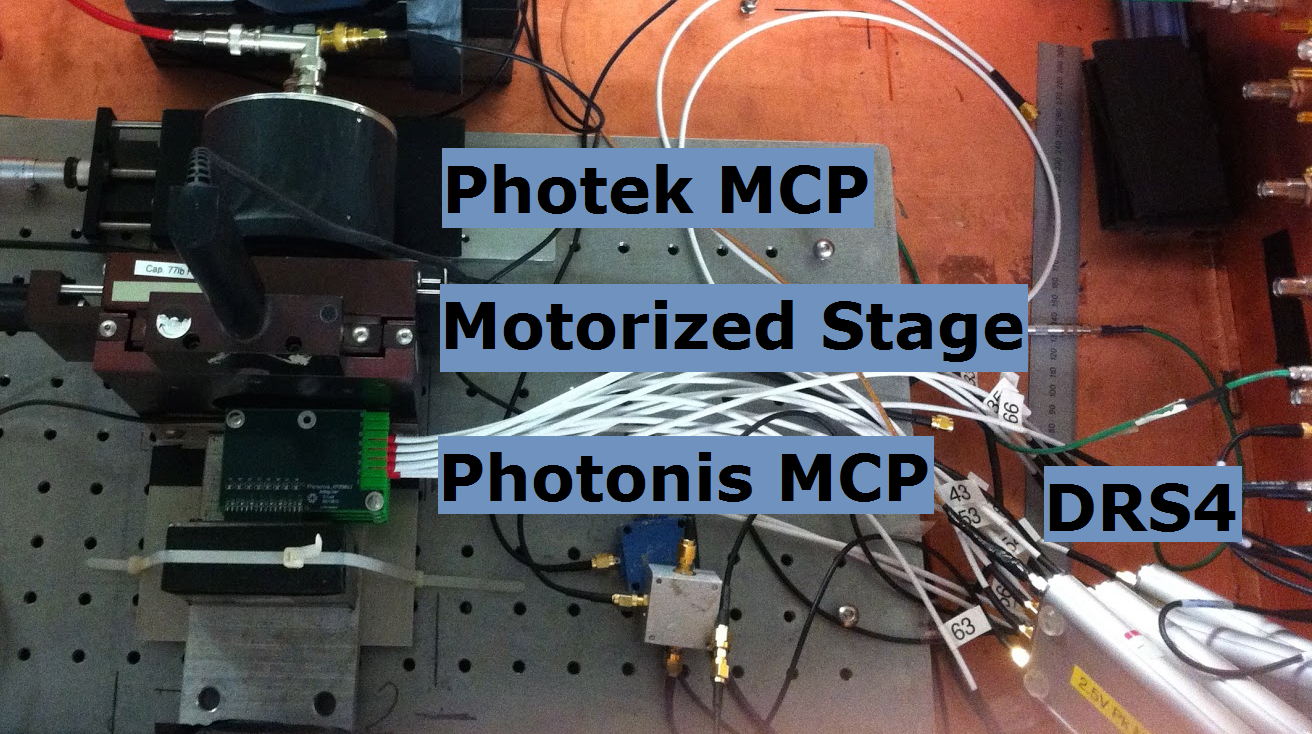
\includegraphics[width=0.8\textwidth]{Images/setup/setup.png} 
\caption{The experimental setup inside of the dark box is shown. The beam direction is from
the bottom of the photograph to the top. The detector elements shown in the
order from upstream to downstream of the beam are: the tungsten absorber, the
Photonis XP85011 MCP-PMT located on the motorized stage, and the Photek 240
MCP-PMT used as a time reference detector. The DRS4 waveform digitizers are also
shown on the lower right side.} 
\label{fig:setup} 
\end{figure} 

An external view
of the Photonis XP85011 MCP-PMT is shown on the left of Figure~\ref{fig:photonis},
and a schematic diagram is shown on the right. There are a total of 64 pixels
arranged in an $8\times8$ square that can be read out individually. For our
experiment, the nine pixels shown within the red square are used. During the
course of the experiment we found that the pixel labelled 44 in
Figure~\ref{fig:photonis} did not function properly and was therefore not used
in the analysis of the data. 

\begin{figure}[htbp] 
\centering
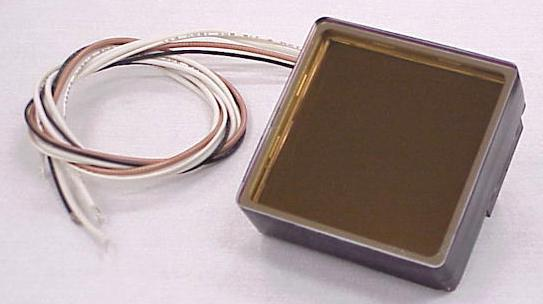
\includegraphics[width=0.49\textwidth]{Images/photonis/photonis.jpg}
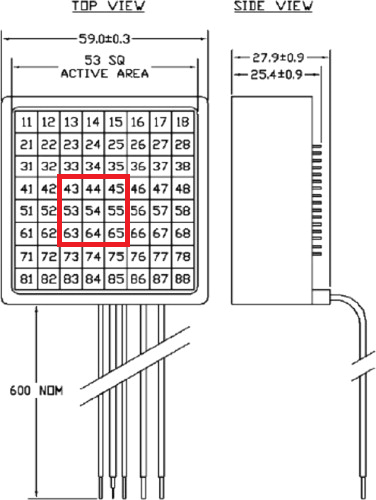
\includegraphics[width=0.49\textwidth]{Images/photonis/photonis2.png}
\caption{The external view of the Photonis XP85011 MCP-PMT is shown on the left, and
the schematic diagram is shown on the right. The red square indicates the pixels
used for the experiment and data analysis.} 
\label{fig:photonis} 
\end{figure}

Four DRS4 high speed waveform digitizers were used to acquire the signals from
the Photek 240 MCP-PMT, the cherenkov counter, and the eight operational
channels from the Photonis XP85011 MCP-PMT. In order to allow a synchronized
readout of four separate DRS4 units we split the signals from the Photek 240
MCP-PMT into four, and connected them to each of the four DRS4 units, thus achieving
a ``calibration'' between the four different units.  

% should draw a diagram of how the channels were distributed among the 4 DRS %units


\section{Event Selection and Pulse Reconstruction}\label{sec:reconstruction}
Reconstruction of the signal pulses and timestamps is performed using the
identical methods described in our past
studies~\cite{Anderson:2015gha,MCPFastCaloNIMA,Ronzhin:2015pba}.
In Figure~\ref{fig:expulse}, we show example pulses from one pixel channel of
the Photonis XP85011 MCP-PMT and the Photek 240 MCP-PMT digitized by the DRS4.

We measure time resolution as the standard deviation of the Gaussian fit to the
time-of-flight distribution $t_0-t_1$, where $t_0$ is the time recorded at the
``start'' detector, and $t_1$ is that of the ``stop'' detector. To assign a time
stamp for each signal pulse, we first determine the time position of the pulse
peak. A Gaussian function is fitted to the pulse maximum using three points
before the maximum of the pulse peak and four points after the maximum. The mean
value of the Gaussian was used as the time stamp for each pulse. A Photek 240
MCP-PMT, whose time resolution was previously measured to be less than
$10$~ps~\cite{Ronzhin:2015pba} was used as a ``start'' signal, while pulses from
individual pixels on the Photonis XP85011 MCP-PMT were used as ``stop'' signals.
More details on the pulse reconstruction algorithms that we use are presented in
Ref.~\cite{MCPFastCaloNIMA}. The integrated charge for each pulse is used as a
proxy for the measured energy deposit in each channel, and is computed using
four time samples before and after the peak of the pulse. Each time sample is
approximately $0.2$~ns in time. Events containing pulses above $500$~mV in
amplitude are rejected as they saturate the DRS4. Only pulses with amplitude
larger than $20$~mV are used for time measurements, to reduce the impact of the
electronics noise in the DRS4. Other event selection and pulse cleaning
procedures are used to eliminate abnormal pulses in the readout, as described
in~\cite{MCPFastCaloNIMA}. 

\begin{figure}[htbp]
  \centering
  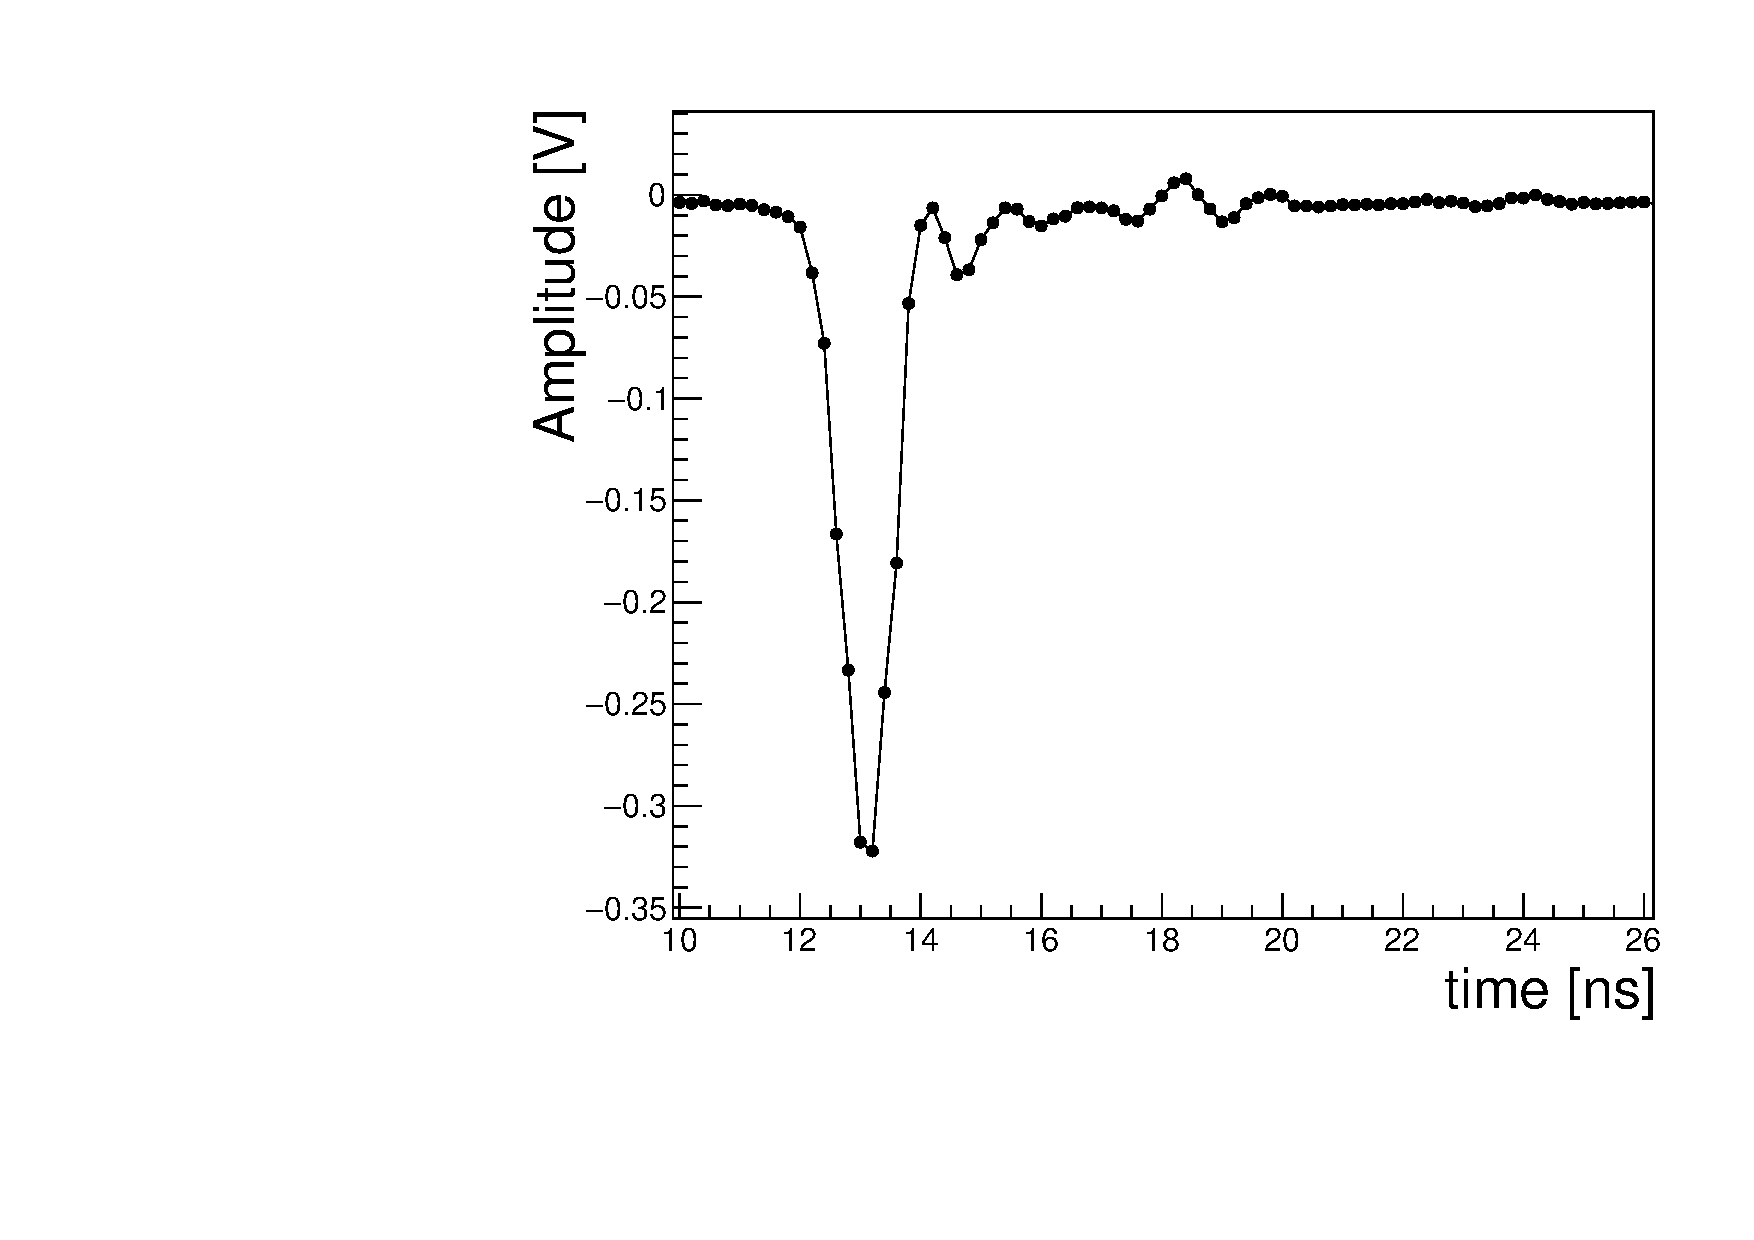
\includegraphics[width=0.49\textwidth]{Images/expulse/pulsepix_30_2_12.pdf}
  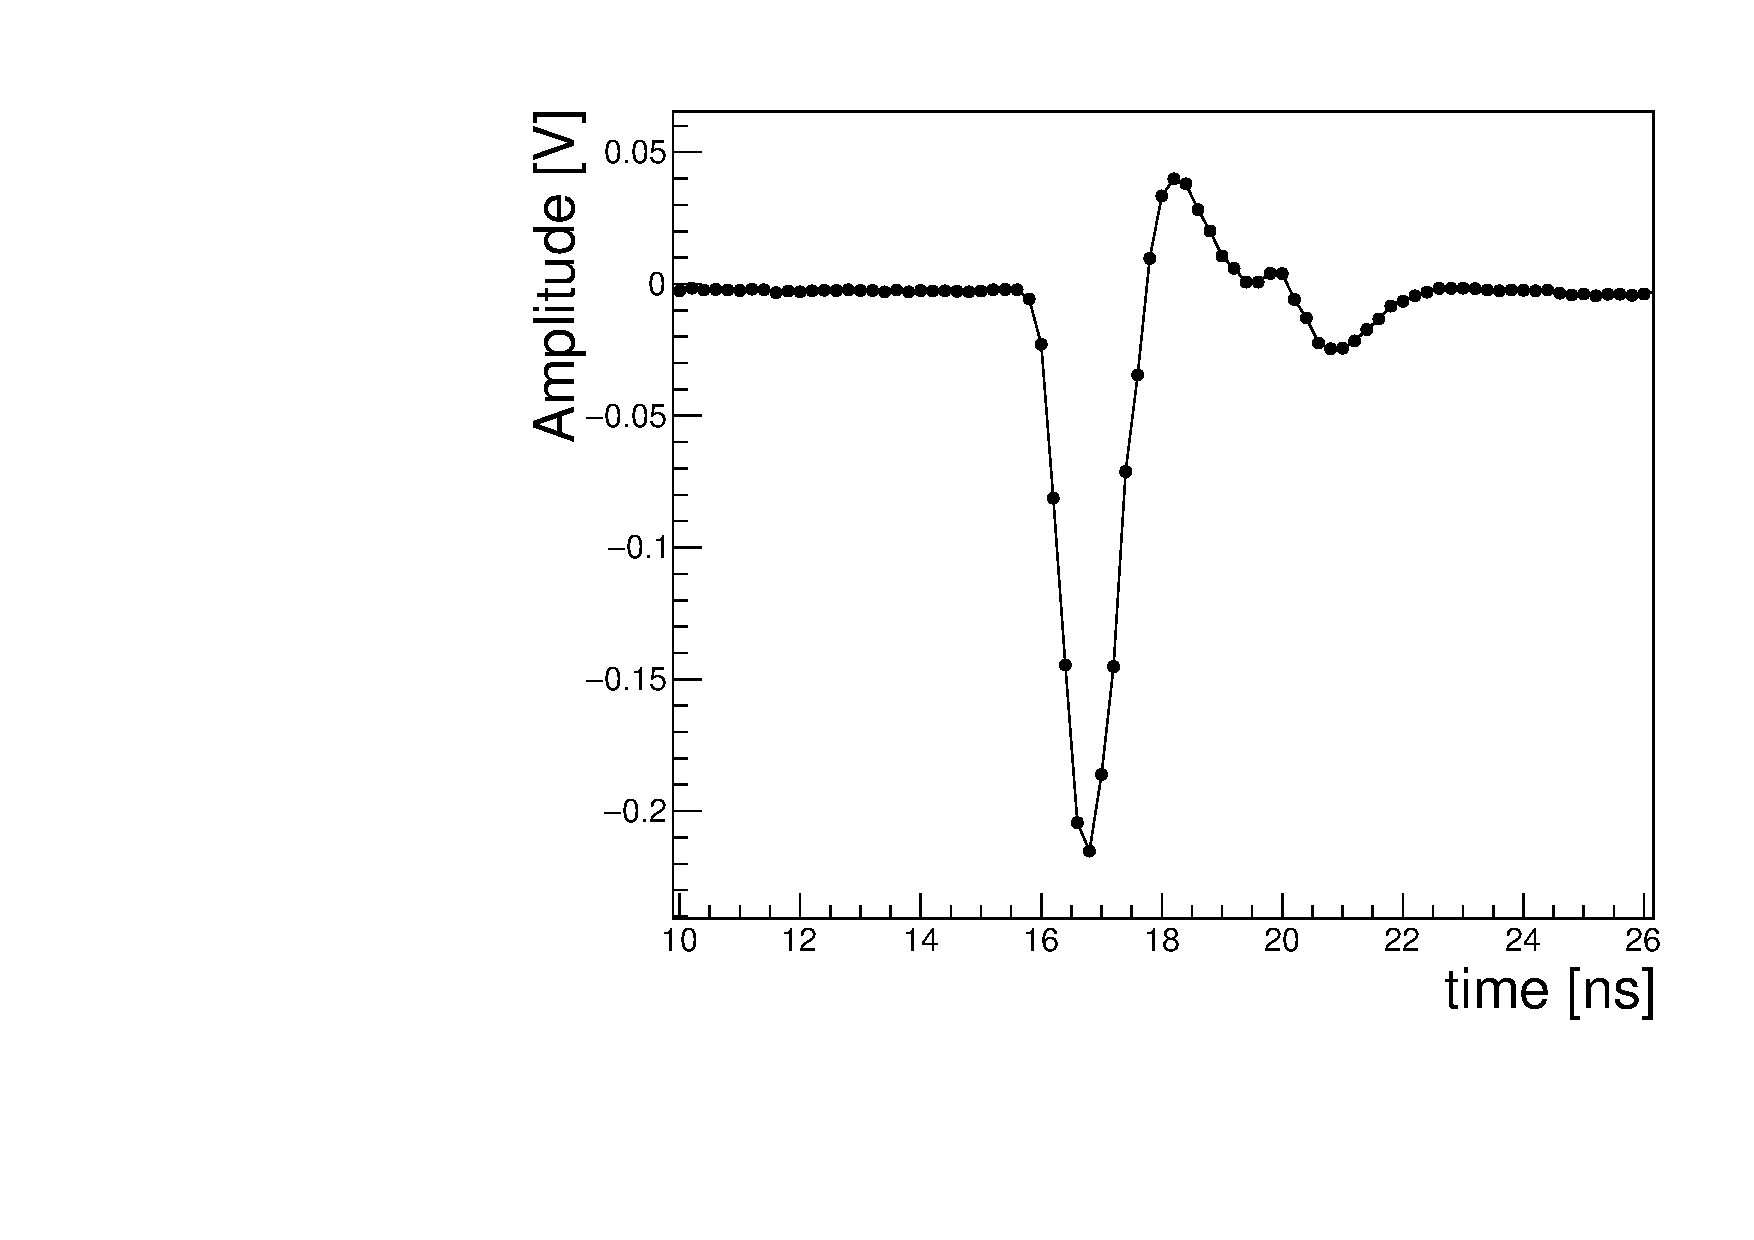
\includegraphics[width=0.49\textwidth]{Images/expulse/pulseref_30_2_10.pdf}
  \caption{\small Example of a digitized signal from a single Photonis pixel
(left) and Photek (right) MCP-PMT following a high-energy electron shower, via DRS4.}
  \label{fig:expulse}
\end{figure}


\section{ Electromagnetic Shower Position Reconstruction and Resolution}\label{sec:position}
The transverse shape of electromagnetic showers is very
well known and has a characteristic width given by the Moliere radius. For
tungsten, the Moliere radius is about $9$~mm and therefore we expect the shower
to be contained within two of the pixels in the Photonis XP85011 MCP-PMT. In
Figure~\ref{fig:exavint}, we show the mean charge measured in each of the pixels
for one example run where the Photonis MCP-PMT was held in a fixed location
approximately centered on the beam. The electron beam has a width of about
$1$~cm. 

\begin{figure}[htbp] 
\centering
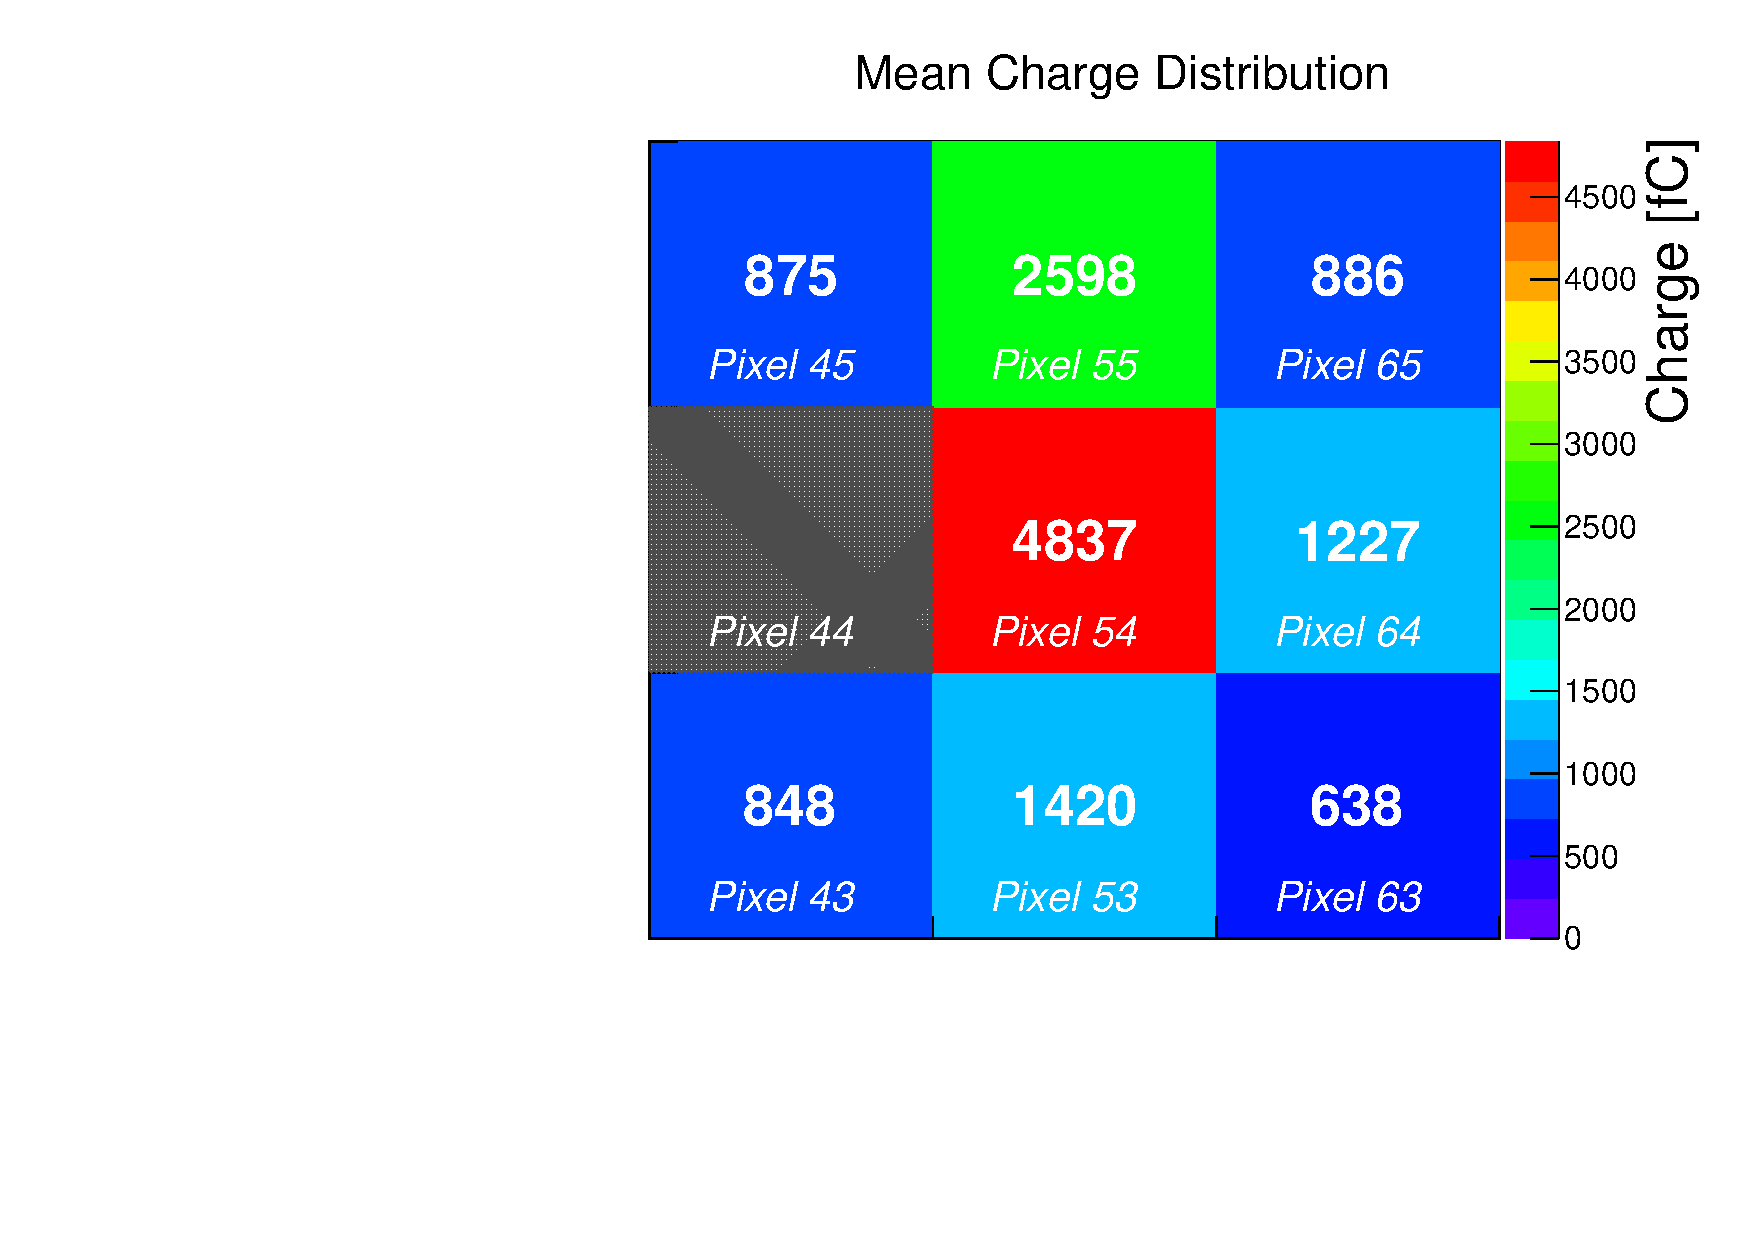
\includegraphics[width=8cm]{Images/exavint/exintrun30.pdf} 
\caption{\small The mean charge measured for each pixel for one example run is shown. During this run, the Photonis MCP-PMT was held in the same location. Based on the distribution
of the mean charge among the pixels, we can infer that the beam center is
located in the upper half of the center pixel. Pixel 44 is not shown as it was
found to be not operational. } 
\label{fig:exavint} 
\end{figure} 

Each electron impacting the shower-maximum detector will induce an
electromagnetic shower, and we define such an occurrence as an event. For each
event, we reconstruct the center position, $\vec{p}$ of the electromagnetic
shower based on the the pixel positions weighted by the corresponding integrated
charge as follows: 
\begin{equation} 
 \vec{\mathbf{{p}}} =
\frac{\sum_{i\in\mathrm{pixels}} Q_{i} \vec{p}_i} {\sum_{i\in\mathrm{pixels}}
Q_{i}} 
\end{equation} 

where $i$ labels the individual pixels, $Q_{i}$ is the charge collected in pixel
$i$, and $\vec{p}_{i}$ is the vector describing the $x$ and $y$ coordinates of
the center of pixel $i$. The origin of the coordinate system is chosen to be at
the lower left corner of the $3\times3$ array of pixels.

Multiple runs were taken scanning different beam positions relative to the
Photonis MCP-PMT by moving the motorized stage. In
Figure~\ref{fig:EMShowerPositions} we show the distributions of the
reconstructed shower positions for three example runs in which the beam was
located near the top, center, and bottom of the center pixel. The distributions
of the reconstructed $y$ coordinate for the three corresponding runs are shown
together in Figure~\ref{fig:EMShowerYPositionComparison}. The measured beam-spot
is observed to move consistent with the known movement of the motorized stage.

\begin{figure*}[htbp] \centering
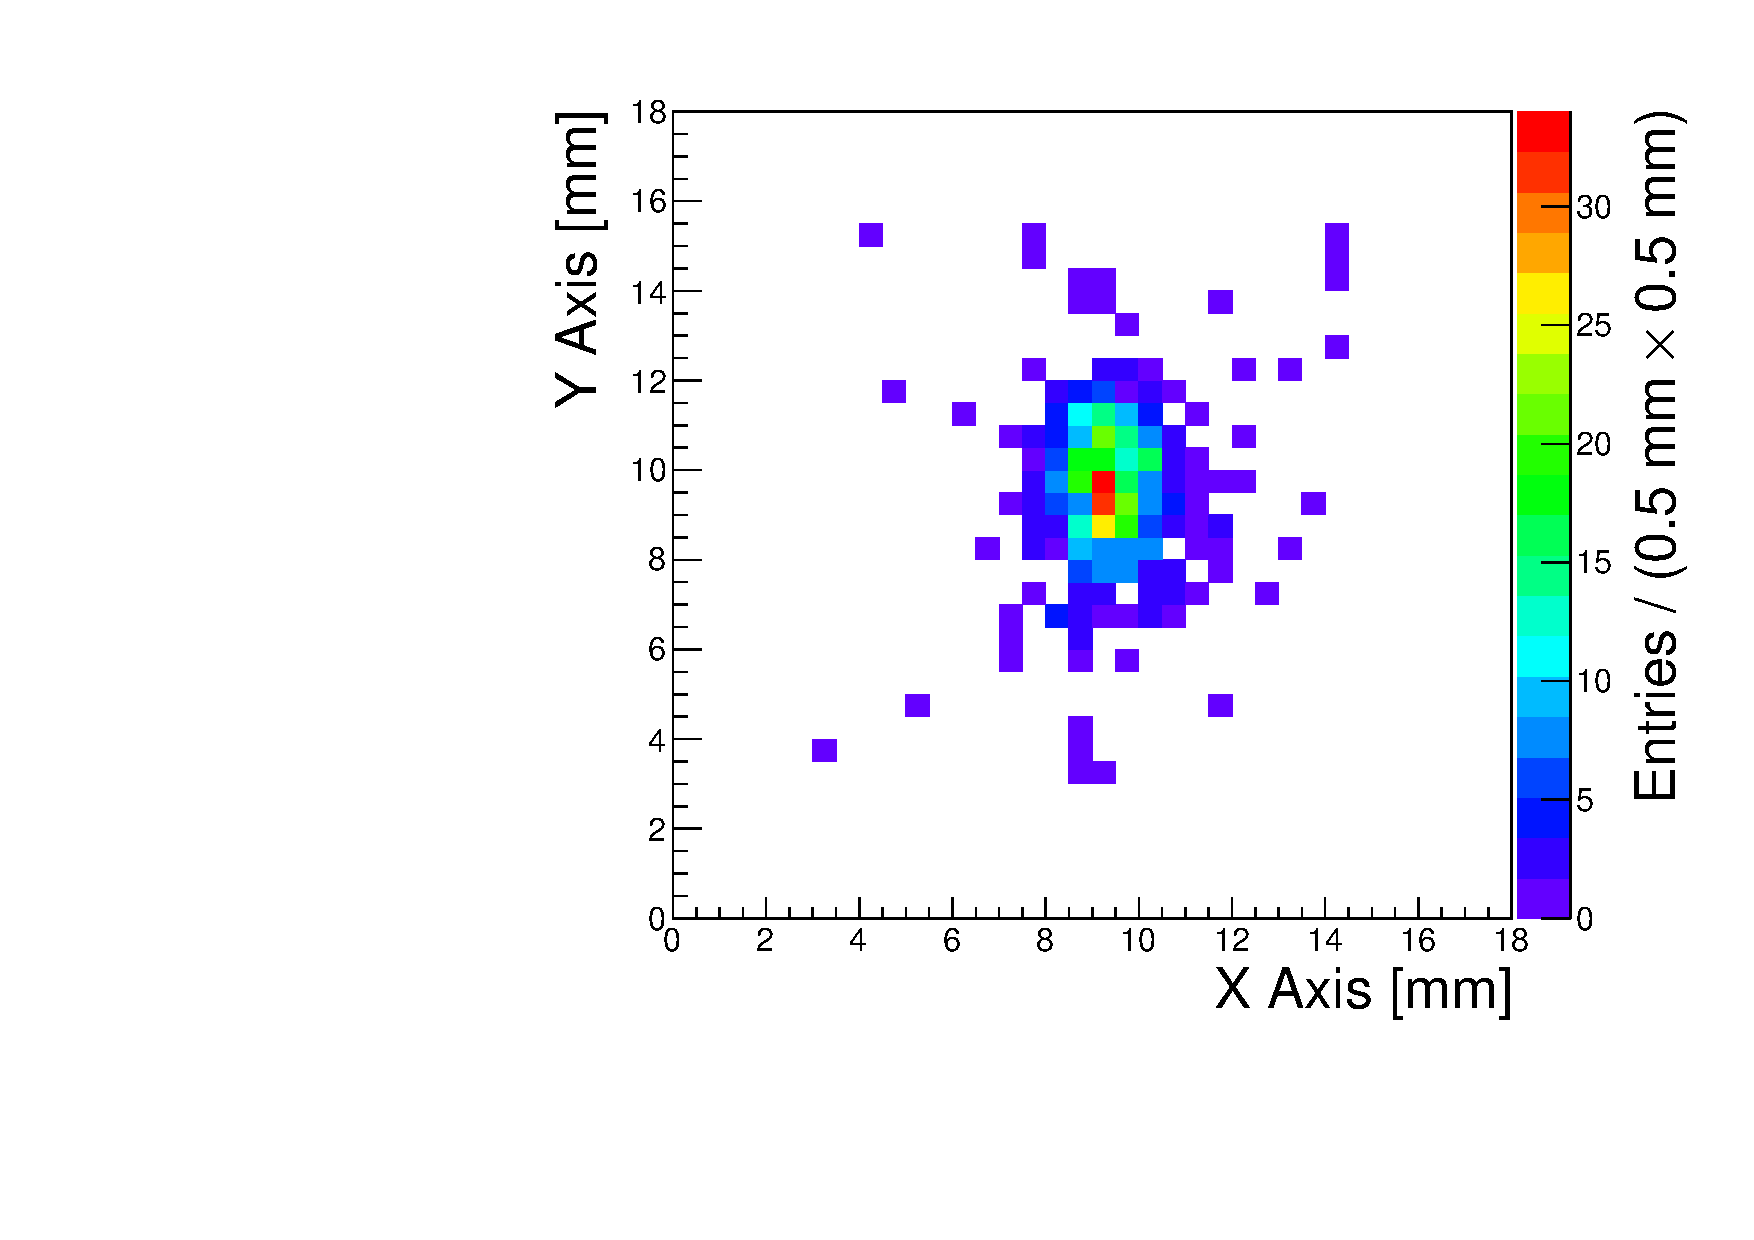
\includegraphics[width=0.49\textwidth]{Images/centers/run30dist.pdf}
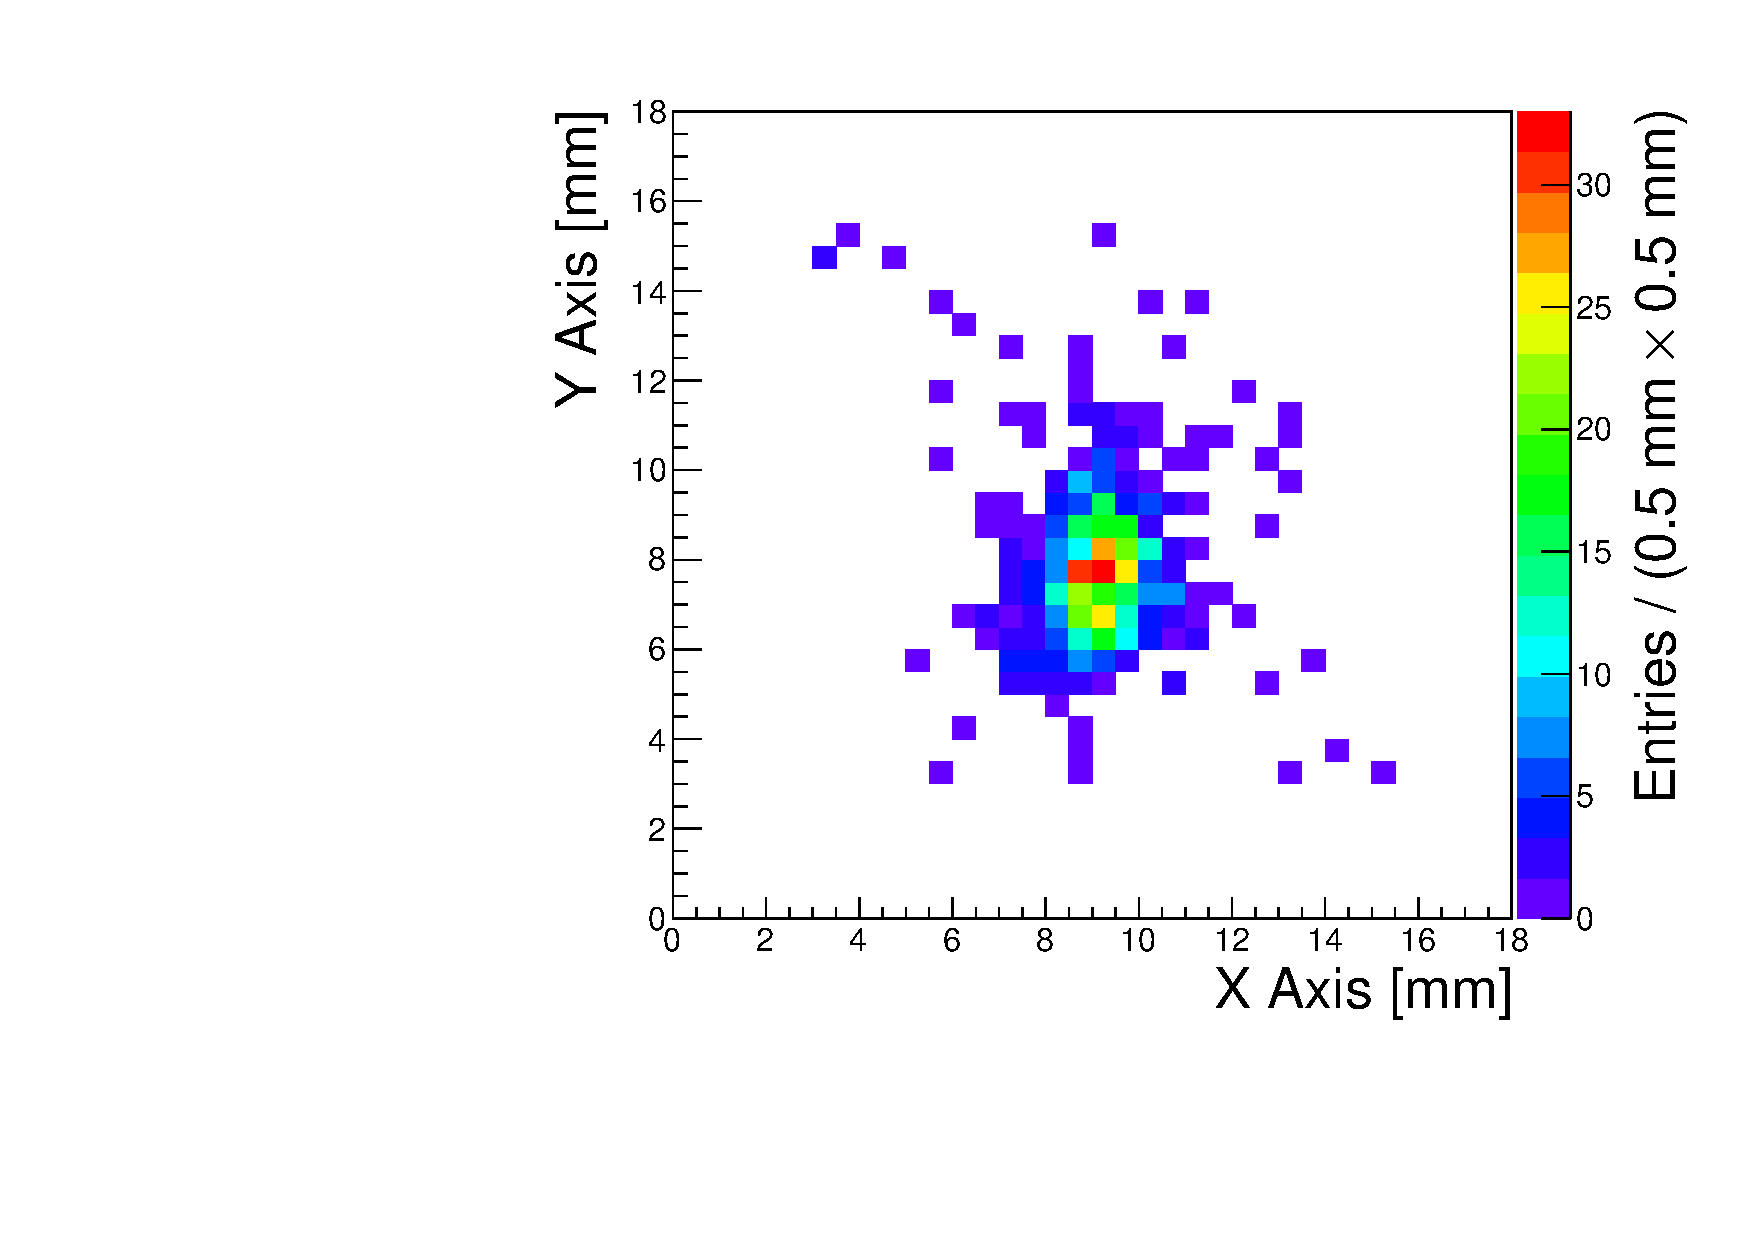
\includegraphics[width=0.49\textwidth]{Images/centers/run32dist.pdf}
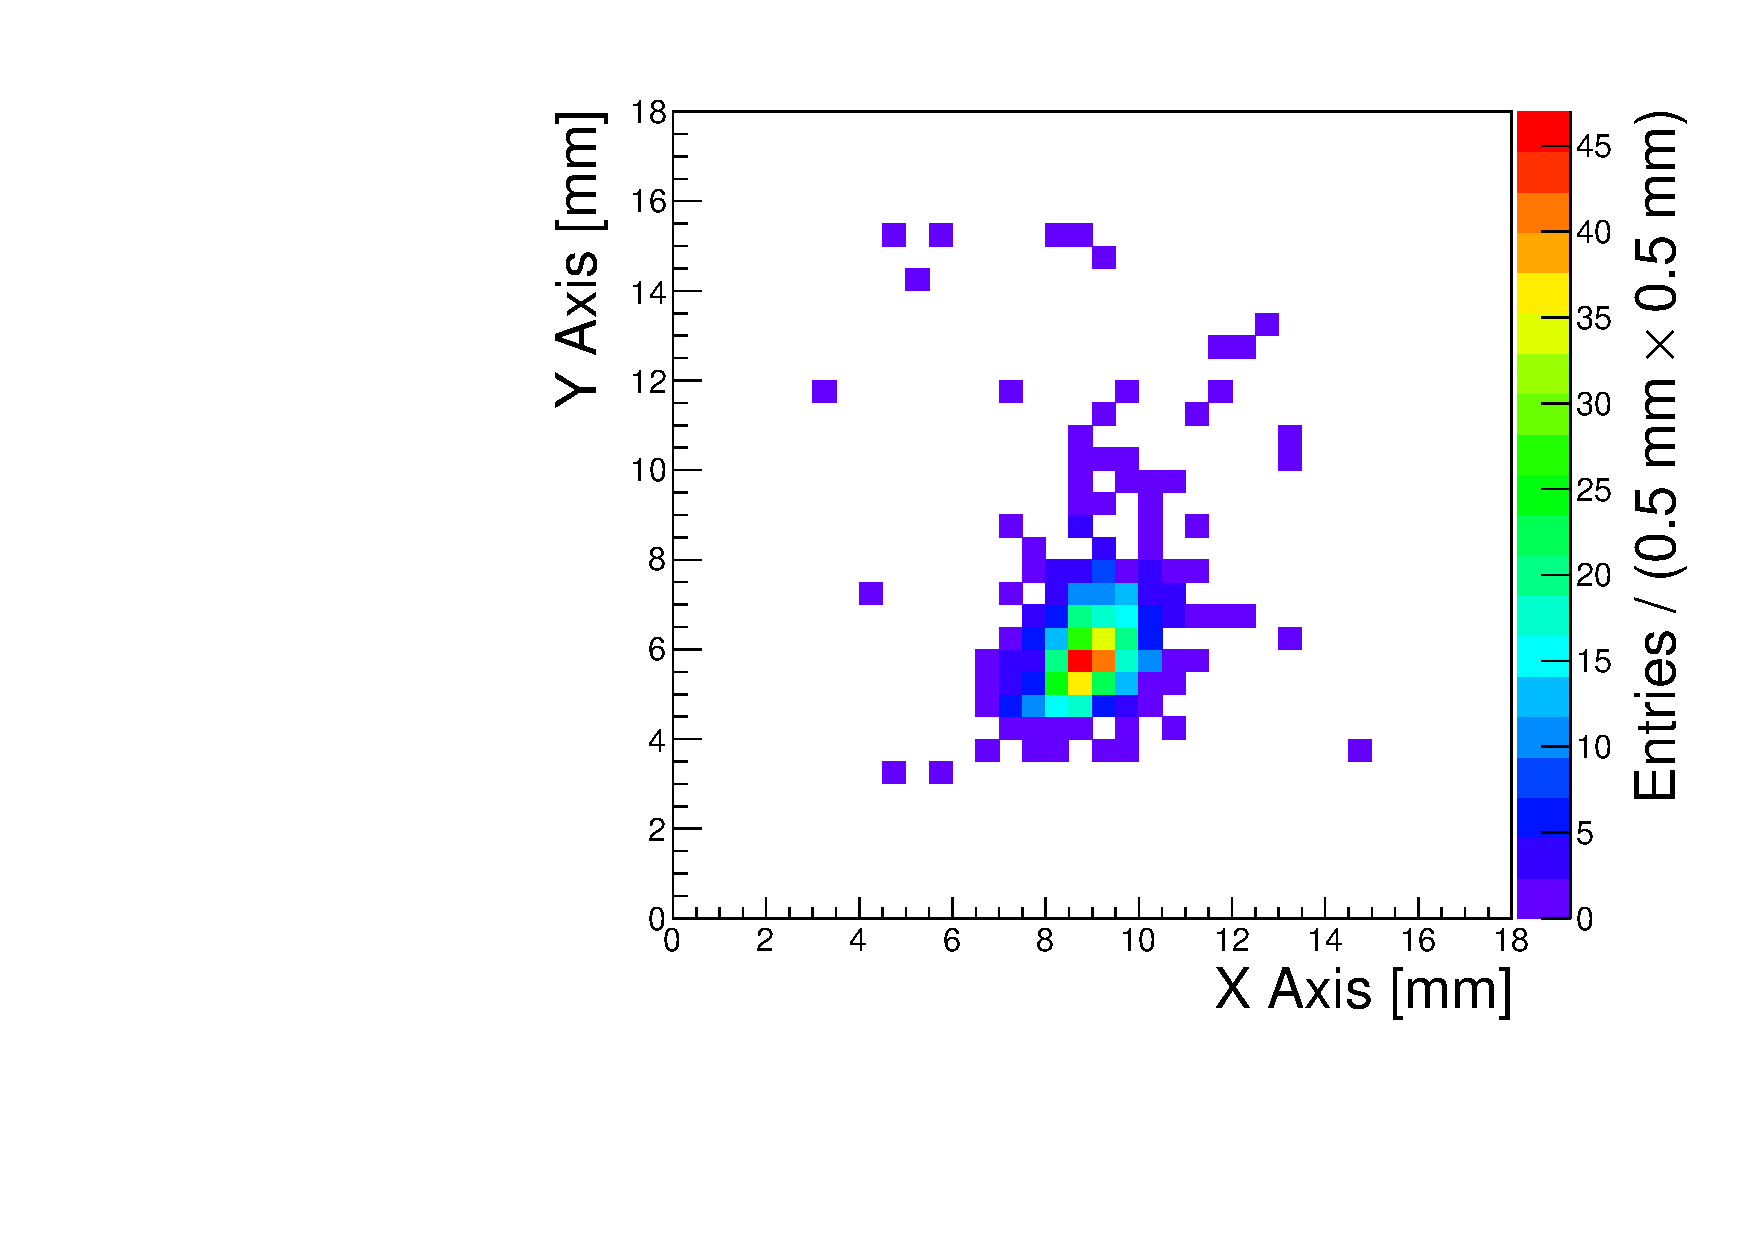
\includegraphics[width=0.49\textwidth]{Images/centers/run34dist.pdf}
\caption{The distribution of reconstructed shower positions is shown for three
runs with the beam centered near the top, center, and bottom of the central
pixel. } \label{fig:EMShowerPositions} \end{figure*} \begin{figure*}[htbp]

\centering
\includegraphics[width=0.75\textwidth]{Images/centers/superimposed.pdf}
\caption{The distributions of reconstructed shower position in the $y$ axis is
shown for the three runs corresponding to the distributions shown in
Figure~\ref{fig:EMShowerPositions}. The measured beam displacements are compared
to the known displacements as recorded by the motorized stage. }
\label{fig:EMShowerYPositionComparison} 
\end{figure*} 

For each run, we determine the center of the beam-spot by fitting the measured
$x$ and $y$ coordinates with a gaussian function. The data from all runs are
combined by considering the measured $x$ and $y$ coordinates relative to the
center of the beam-spot (see Fig~\ref{fig:ResolutionMeasurement}). We model the
distribution of measured coordinates as a convolution of a flat distribution
with width equal to the measured dimensions of the scintillator trigger and a
gaussian resolution function. A maximum likelihood fit is performed on the data
using this model, and the position resolution of the detector is measured as the
width of the gaussian resolution function. We measure the position resolution as
$0.55\pm0.2$~mm in $x$-coordinate, and $0.91\pm 0.01$~mm in $y$-coordinates.

\begin{figure*}[htbp] \centering
\includegraphics[width=0.49\textwidth]{Images/XYResolution/X_Resolution_fixedTrigger.pdf}
\includegraphics[width=0.49\textwidth]{Images/XYResolution/Y_Resolution_fixedTrigger.pdf}
\caption{The distributions of the measured $x$ (left) and $y$ (right)
coordinates are shown along with the fit to the resolution model. The position
resolution of the EM shower as measured by the MCP-PMT detector is determined from
the fit to the resolution model. } \label{fig:ResolutionMeasurement}
\end{figure*}

\section{Electromagnetic Shower Time Resolution} \label{sec:timing} 
The timestamps for each event for individual pixels of the Photonis MCP-PMT are
reconstructed as described in Section~\ref{sec:reconstruction}. We reconstruct
the timestamp of the entire electromagnetic shower using the same energy
weighting procedure that was used above for the shower position reconstruction:

\begin{equation} t =\frac{\sum_{i\in\mathrm{pixels}} Q_{i} t_{i}}
{\sum_{i\in\mathrm{pixels} Q_{i}}}, 
\label{eqn:EnergyWeightedTimestamp}
\end{equation} 

where $i$ labels the individual pixels, $Q_{i}$ is the charge
collected in pixel $i$, and $t_{i}$ is the reconstructed time-stamp for pixel
$i$. Alternatively, we also study the time resolution using the single pixel
with the highest energy deposit measurement. In Figure~\ref{fig:exdt} we show
the time distributions for these two methods of shower time reconstruction.

\begin{figure*}[htbp] 
\centering
\includegraphics[width=8cm]{Images/exdt/exdtHI.pdf}
\includegraphics[width=8cm]{Images/exdt/exdtWI.pdf} 
\caption{\small The time distributions obtained using the highest energy pixel (left) and the energy weighted algorithm (right) are shown for one example run. The distributions are
fitted with Gaussian models, and the width parameter of the Gaussian is
displayed on the plot.} 
\label{fig:exdt} 
\end{figure*} 

In Figure~\ref{fig:wtres}, we compare the time resolution for electromagnetic
showers measured using the two methods described above. The time resolution for
the pixel with the largest energy deposit is around $70$~ps and $85$~ps,
depending on the run. Using the energy weighted algorithm improves the time
resolution consistently to about $50$~ps. 

\begin{figure}[htbp] 
\centering
\includegraphics[width=8cm]{Images/wtres/tresperrun.pdf} 
\caption{\small Time resolution found for each run. The time-stamp obtained using the energy weighting method yields time resolutions consistently below $60$~ps. The time resolution measured using the single pixel with the largest signal is significantly worse.} 
\label{fig:wtres} 
\end{figure} 

We note that the time measurement made using the Photonis MCP-PMT typically exhibit
a dependence on the pulse amplitude or integrated charge. This dependence is
shown on the left of Figure~\ref{fig:dt-int}, and is observed to be
approximately the same for all pixels. We perform a correction to the time
measurement based on the measured integrated charge, and we verify that the
correction does flatten the dependence of the time measurement on the integrated
charge as shown on the right panel of Figure~\ref{fig:dt-int}. After performing
this time measurement correction, the time resolution measurements improve to
about $35$~ps and is shown in Figure~\ref{fig:calib}. We performed two sets of
correction procedures. In one set, labelled as ``Self-Calibrated'', an
independent correction is derived for each run and for each pixel. In the second
set, labelled as ``Calibrated'', a single correction is obtained for each pixel
from a single run, and this correction is applied to all other runs.
Figure~\ref{fig:calib} shows that this single correction is applicable to all
other runs without loss of the precision of the measurements. 

\begin{figure*}[htbp] 
\centering
\includegraphics[width=8cm]{Images/dt-int/dtint30_o22.pdf}
\includegraphics[width=8cm]{Images/dt-int/dtint30_c22.pdf} 
\caption{The correlation between the time measurement and the measured integrated charge is
shown on the left for one example pixel. The same correlation after performing
the time measurement correction is shown on the right. } 
\label{fig:dt-int}
\end{figure*} 

\begin{figure}[htbp] 
\centering
\includegraphics[width=8cm]{Images/calibtres/timerescalib.pdf} 
\caption{ The time resolution of the electromagnetic shower for various runs is
shown after performing the time measurement correction based on the measured
integrated charge. } 
\label{fig:calib} 
\end{figure} 

Finally, we study the dependence of the electromagnetic shower time resolution
as a function of the number of pixels included in the energy-weighted algorithm.
Figure~\ref{fig:sqrtN} shows this dependence for one example run. We observe
that the time resolution improves according to a $1/\sqrt{N}$ scaling up to
about 5--6 pixels, and then becomes flat as we include more pixels. The
initial $1/\sqrt{N}$ scaling is encouraging as it indicates that the time jitter across
different pixel channels arise primarily from uncorrelated sources, and that
further granularity may improve the time resolution provided that the signal is
sufficiently large compared to noise. As the majority of the shower is
covered by the pixels closest to the center of the shower, it is not surprising
that we do not observe any improvement from the inclusion of additional pixels.

\begin{figure}[htbp]
  \centering
  \includegraphics[width=8cm]{Images/sqrtN/t1065_run_38_Dt_IWP.pdf}
  \caption{ The time resolution is plotted as a function of the number of pixels
    included in the energy-weighted algorithm for one example run. }
  \label{fig:sqrtN}
\end{figure}

\section{Summary}
We continue our studies on the development of future electromagnetic 
calorimeters capable of high precision energy and time measurements.
Such calorimeters should provide both spatial resolution below the $\mathrm{mm}$
level and time resolution of $20-30$~ps, in order to mitigate the detrimental effects
of pileup. A highly granular readout is required to achieve these goals. 

We report our results on position and time resolution measurements of a
secondary emission based calorimeter prototype that used the Photonis XP85011
MCP-PMT as the active element. Using a pixelated readout of the MCP-PMT we
obtain highly granular information of the shower development in the
transverse plane. Combining the measurements from a $3\times3$-channels readout
we obtain a sub-millimeter precision for position measurement, which far exceeds
the 6~mm size of individual pixels. While the more granular readout degrades
the signal to noise for each individual pixel, we demonstrate that a proper combination from 
independent readout channels preserves good time resolution. We show that the time resolution 
of the measurements improves with the increase in the number of pixels used as 
$1/\sqrt{N}$, and using all pixels we achieve a time resolution of $30-40$~ps. 
In future measurements we intend to include larger prototypes with several layers of active
material, that will allow us to explore the longitudinal development of the
showers.

\section{Acknowledgements}
We would like to thank Erik Ramberg for supporting 
our work, and Aria Soha and the FTBF test beam facility for the good beam
delivery and control. Thanks to Ewa Skup and Geoff Savage for help with
operation of Cherenkov counters, and to Todd Nebel for organizing and providing
supporting equipment at FTBF. 

This work is supported by funding from Fermi Research Alliance, LLC under
Contract No. DE-AC02-07CH11359 with the United States Department of Energy, and
from California Institute of Technology High Energy Physics under Contract
DE-SC0011925 with the United States Department of Energy.

\clearpage
\chapter{Silicon Based Sampling Calorimeters}\label{sil-cal}
Future colliders, including the high luminosity upgrade of the Large Hadron
Collider (HL-LHC) at CERN, will operate with an order of magnitude higher
instantaneous luminosity compared to what has been achieved at the LHC so far.
With the increased instantaneous luminosity the rate of simultaneous
interactions per bunch crossing (pileup) is projected to reach an average of 140
to 200. The large amount of pileup increases the likelihood of confusion in the
reconstruction of particles from the hard scatter interaction with those
produced in different pileup interactions. The ability to discriminate between
jets produced in the events of interests, especially those associated with the
vector boson fusion processes, and jets produced by pileup interactions will be
degraded. The missing transverse energy resolution will deteriorate, and several
other physics objects performance metrics will suffer.

One way to mitigate the pileup confusion effects, complementary to precision
tracking methods, is to perform a time of arrival measurement associated with a
particular layer of the calorimeter, allowing for a time assignment for 
charged particles and photons. Such a measurement with a precision of about
20-30 ps, when unambiguously associated to the corresponding energy measurement,
will reduce the effective amount of pileup by a factor of 10, given that the
spread in collision time of the pileup interactions at HL-LHC is foreseen to be
approximately 200~ps. The association of the time measurement with the energy
measurement is crucial, and leads to a prototype design that calls for  time
and energy measurements to be performed in the same detector element. Since both
the energy and time measurement are performed in the same detector
element\footnote{If there are no overlapping energy deposits in the same
detector element from multiple particles.}, once
an energy deposit is identified as originating from a pileup interaction, it can
be unambiguously removed from event reconstruction. 

Several alternative options to combine high resolution energy and timing
measurements for calorimetry have been reported in Refs.~\cite{Anderson:2015gha,
MCPFastCaloNIMA, Ronzhin2015288, Ronzhin201552, Brianza2015216, sixie, spiropulu}. In this
article, we describe the continuation of this program of study using a
calorimeter prototype employing a 300~$\mu$m thick silicon pad sensor of
$6\times 6$~mm$^2$ size as the active element. Silicon-based calorimeters have
recently become a viable choice for future colliders due to the radiation
hardness of silicon, and the ability to construct highly granular
detectors~\cite{Adloff:2011ha}. An important example is the forward calorimeter
proposed for the CMS Phase 2 Upgrade~\cite{Butler:2020886}. We study the timing
properties of silicon-based calorimetery using a prototype composed of tungsten
absorber and a silicon sensor produced by Hamamatsu~\cite{hamamatsu}. A similar
test was previously conducted at the CERN North Area, with a lead absorber
followed by silicon sensors of 120-320~$\mu$m thickness~\cite{akchurin, rusack}.

The paper is organized as follows. General silicon timing properties and bench
test results are described in Section~\ref{sec:siliconpad}. The test beam setup
and experimental apparatus are presented in Section~\ref{sec:tbeam}. The results
of the test beam measurements are presented in Section~\ref{sec:results}.
Sections~\ref{sec:discussion}~and~\ref{sec:conclusion} are devoted to discussion
and conclusion, respectively.

\section{General Properties of Silicon Timing and Bench Test Studies}
\label{sec:siliconpad}

For our measurements, we used a silicon sensor produced by
Hamamatsu~\cite{hamamatsu}. The thickness of the silicon was measured to be ~325
$\mu$m. The transverse size of the sensor is 6x6 mm$^2$. The negative bias
voltage was applied to the p-side of the silicon. The capacitance
of the silicon diode is measured as a function of the bias voltage
and shown in Figure~\ref{fig:SiliconDiode}. We observe that the silicon
is fully depleted above about $120$~V. Timing measurements are expected
to improve with larger bias voltage as the the carrier velocity increases.

The electric diagram of the silicon
diode connections is presented in Figure~\ref{fig:SiliconPad}. Attention was
paid to provide good filtering for bias voltage, to reduce ground loop effects, and
to minimize inductive loop for the signal readout. The timing characteristics
of the signal pulses are dominated primarily by properties of the
silicon sensor rather than the details of the circuit.

\begin{figure}[htbp] 
\centering
\includegraphics[width=0.8\textwidth]{plots/SiliconDiodeCV_v3.pdf} 
\caption{The measured capacitance as a function of the applied bias voltage.} 
\label{fig:SiliconDiode} 
\end{figure} 

The silicon diode was placed inside a light-tight box of thickness $1.5$~cm,
which also provides electromagnetic shielding. The box is made of 0.2~mm steel.
The bias voltage was supplied to the circuitry by a cable with a balun filter,
terminated with an SHV connector. The silicon diode output signal is read out
through an SMA connector electrically grounded to the box. The dark current was
measured at several values of the bias voltage. The maximum value of the dark
current was less than $1.0$~nA at $-500$~V, which is the largest bias voltage
used in the measurements reported in this paper. The silicon box and bench test
setup are presented in Figure~\ref{fig:SiliconPad}. 

\begin{figure}[htbp] 
\centering
\includegraphics[width=0.60\textwidth]{plots/SiliconDiodeDiagram.pdf} 
\includegraphics[width=0.39\textwidth]{plots/SiliconDiodeBox.jpg} 
\caption{The electric diagram for the silicon diode connections (left). External
view of the box with silicon diode, and the bias voltage connection is shown
below it (right).} 
\label{fig:SiliconPad} 
\end{figure} 

The signals from the silicon sensor were amplified by two fast, high-bandwidth
pre-amplifiers connected in series. The first amplifier is an ORTEC VT120C
pre-amplifier, and the second amplifier is a Hamamatsu C5594 amplifier. Using a
pulse-generator, we measured the combined gain of the two amplifiers in series
as a function of the input signal amplitude and found some degree of
non-linearity for typical signals produced by the silicon sensor under study,
and we corrected for them.

%. The measured gain ranged from $200$ for signals with
%input amplitude around $0.15$~mV to $650$ for signals with amplitude around $10$~mV.

\section{Test-beam Setup and Experimental Apparatus }
\label{sec:tbeam}

We performed the test-beam measurements at the Fermilab Test-beam Facility
(FTBF) which provided a proton beam from the Fermilab Main Injector accelerator
at $120$~GeV, and secondary beams composed of electrons, pions, and muons of
energies ranging from $4$~GeV to $32$~GeV. A simple schematic diagram of the
experimental setup is shown in Figure~\ref{fig:BeamSchematicDiagram}. A small
plastic scintillator of transverse dimensions $1.8$~mm$\times 2$~mm is used as a
trigger counter to initiate the read out of the data acquisition (DAQ) system
and to select incident beam particles from a small geometric area, allowing us to center the 
beam particles on the silicon sensor. Next, we place a stack of tungsten absorbers of various thicknesses for
measurements of the longitudinal profile of the electromagnetic shower. The
silicon pad sensor is located within a metal box covered by copper foil, and is
placed immediately downstream of the absorber plates. Finally, a Photek 240
micro-channel plate photomultiplier detector~\cite{Anderson:2015gha,
MCPFastCaloNIMA, Ronzhin2015288,Ronzhin201552} is placed furthest downstream,
and serves to provide a very precise reference timestamp. Its precision was
previously measured to be less than $10$~ps~\cite{Ronzhin2015288}. 
A photograph showing the various
detector components is presented in Figure~\ref{fig:BeamPhotoDiagram}. A
differential Cherenkov counter is located further upstream of our experimental
setup and provides additional particle identification capability. More
details of the experimental setup are described in our previous studies using
the same experimental facility in references~\cite{Anderson:2015gha,
MCPFastCaloNIMA, Ronzhin2015288,Ronzhin201552}.

\begin{figure}[htbp] 
\centering
\includegraphics[width=0.65\textwidth]{plots/BeamSchematicDiagram.pdf} 
\caption{A schematic diagram of the test-beam setup is shown. The $t_0$ and $t_1$ are defined in Section~\ref{sec:results}.} 
\label{fig:BeamSchematicDiagram} 
\end{figure} 

\begin{figure}[htbp] 
\centering
\includegraphics[width=0.65\textwidth]{plots/BeamPhotoDiagram.pdf} 
\caption{Test beam setup.} 
\label{fig:BeamPhotoDiagram} 
\end{figure} 

The DAQ system is based on a CAEN V1742 digitizer board~\cite{CAENDRS}, which
provides digitized waveforms sampled at 5 GS/s. The metal box containing the
silicon sensor was located on a motorized X-Y moving stage allowing us to change
the location of the sensor in the plane transverse to the beam at an accuracy
better than $0.1$~mm. A nominal bias voltage of $500$~V was applied to deplete
the silicon sensor in most of the studies shown below, unless noted otherwise.


\section{Test Beam Measurements and Results} 
\label{sec:results} 

Measurements were performed in 2015, using the primary 120~GeV proton beam, and secondary
beams provided for the FTBF. Secondary beams with energies ranging from 4
GeV/c$^2$ to 32 GeV/c$^2$ were used. Electron purity for those beams ranges
between $70\%$ at the lowest energy to about $10\%$ at the highest energy.
Stacks of tungsten plates with varying thicknesses were placed immediately
upstream of the silicon device in order to measure the response along the
longitudinal direction of the electromagnetic shower. The radiation length of
tungsten is 3.5~mm, and the Moliere radius is 9.3~mm. The tungsten plate size is
sufficient to fully contain the shower in the transverse dimension. Signals from
the silicon sensor and the Photek MCP-PMT are read out and digitized by the CAEN
V1742 digitizer, and example signal waveforms are shown in
Fig.~\ref{fig:pulses}. The signal pulse in the silicon sensor has a rise time of
about $1.5$~ns, and a full pulse width of around $7$~ns. This rise time is
consistent with a time constant of a silicon sensor coupled to a 50~Ohm amplifier.

\begin{figure}[htbp] 
\centering
\includegraphics[width=0.45\textwidth]{plots/ExampleSiliconPadPulse_6X0_16GeV.pdf} 
\includegraphics[width=0.45\textwidth]{plots/ExamplePhotekPulse.pdf} 
\caption{Examples of the signal pulse waveform for the silicon sensor (left) and
the Photek MCP-PMT (right) digitized by CAEN V1742 digitizer board. The bias
voltage applied to the silicon pad sensor is~$500$~V.} 
\label{fig:pulses} 
\end{figure} 

The CAEN digitizer is voltage and time calibrated using the  procedure
described in Ref.~\cite{Kim201467}. The total collected charge for each signal
pulse is computed by integrating a $10$~ns window around the peak of the pulse.
The time for the reference Photek MCP-PMT detector is obtained by fitting the
peak region of the pulse to a Gaussian function and the mean parameter of the
Gaussian is assigned as the timestamp $t_0$. The time for signals from the
silicon sensor is obtained by performing a linear fit to the rising edge of the
pulse and the time at which the pulse reaches 30\% of the maximum amplitude is
assigned as its timestamp $t_1$. We measured the electronic time resolution
of the CAEN V1742 digitizer as $\sim$4~ps and neglected its impact on the timing
measurements described below.

Electrons were identified by requiring that the signal amplitude of the gas Cherenkov counter
provided by the FTBF and the Photek detector located further
downstream of the silicon sensor exceed certain thresholds because electromagnetic showers induced by electrons
produce significantly larger signals, while pions produce much smaller signals. After imposing the electron identification requirements the electron purity is between $80\%$ and $90\%$ for all beam
conditions. The purity was determined by comparing the calorimetric measurements with those 
from the Cherenkov detector.

We begin by establishing the signal characteristics of a minimum-ionizing
particle (MIP) using beams of $120$~GeV protons and $8$~GeV electrons with no
absorbers upstream of the silicon pad sensor. To separate MIP signals from
noise, we first collect data events with no beam and random trigger. The charge
distribution for these noise runs is presented in Fig.~\ref{fig:noise}. As expected,
the charge distribution is centered at $0$, and the RMS is about
$2$~fC. 

\begin{figure}[htbp] 
\centering
\includegraphics[width=0.45\textwidth]{plots/NoiseNoBeam_charge.pdf} 
\caption{The distribution of charge integrated in the silicon sensor is shown for data events with no beam and random trigger. } 
\label{fig:noise} 
\end{figure} 

In Figure~\ref{fig:MIP}, we show silicon sensor response to $120$~GeV protons
and $8$~GeV electrons without any absorber. We observe very similar response for
these two cases, and measure peak integrated charge of $4.5$~fC and $5.0$~fC
respectively. The measured signal is corrected for the gain of the amplifiers
used, and hence is the output charge of the silicon sensor. We expect peak charge
of $28,000$ and $31,000$ electron-hole pairs in a $325$ $\mu$m thick silicon
detector for ionizing particles with Lorentz factor $\gamma=120$ (protons) and $16,000$
(electrons)~\cite{Agashe:2014kda}, which is in a good agreement with the measured
values. Having established the absolute scale of the response using single
particles, in our remaining studies we normalize all charge measurements to the
$120$ GeV proton signal, which we refer to in the following as
$\mathrm{Q}_{\mathrm{MIP}}$. 
\begin{figure}[htbp] 
\centering
\includegraphics[width=0.45\textwidth]{plots/Proton_charge.pdf} 
\includegraphics[width=0.45\textwidth]{plots/Electron_0X0_charge.pdf} 
\caption{The distribution of charge integrated in the silicon sensor is shown
for a beam of $120$~GeV protons (left) and $8$~GeV electrons (right) without any
absorber upstream of the silicon sensor. These conditions mimic the response of the silicon sensor to a
minimum-ionizing particle. All triggered events were used in these
distributions.} 
\label{fig:MIP} 
\end{figure} 
We study the response of the silicon sensor to electron beams of various
energies after 6 radiation lengths ($X_0$) of tungsten absorber. The silicon
sensor is expected to be sensitive to the number of secondary electrons produced
within the electromagnetic shower, and therefore its response is expected to
scale up with higher incident electron energy. In
Figure~\ref{fig:ChargeDistributionExample}, we show an example of the integrated
charge distribution measured in the silicon sensor after 6 radiation lengths of
tungsten, for runs with $32$~GeV electrons. We show the mean and RMS of
these distributions as a function of incident electron beam energy in
Figure~\ref{fig:ChargeDistributionExample}. The uncertainties plotted show the RMS of the
charge distribution. Since the electron beam profile and purity varies at different beam energies, we collected between 10 and 50 thousand events for each beam energy, in order to ensure sufficiently large data samples. We observe a fairly linear depedence between the measured
charge and the incident beam energy, for beam energies between $4$~GeV and
$32$~GeV. 
\begin{figure}[htbp] 
\centering
\includegraphics[width=0.49\textwidth]{plots/Electron_6X0_32GeV_chargeMIP.pdf} 
\includegraphics[width=0.49\textwidth]{plots/MIPVsEnergyAt6X0.pdf} 
\caption{ Left: An example of the distribution of integrated charge in the
silicon sensor for 32 GeV electrons and $6$~$X_0$ absorber shown in units of 
$\mathrm{Q}_{\mathrm{MIP}}$. Right: The integrated charge in the silicon sensor 
expressed in units of $\mathrm{Q}_{\mathrm{MIP}}$
is shown for the same $6$~$X_0$ absorber as a function of the electron beam energy. 
The uncertainty bands show the RMS of the measured charge distribution. The red line
is the best fit to a linear function..} 
\label{fig:ChargeDistributionExample}
\end{figure}
We also measure the time resolution between the silicon sensor and the Photek
MCP-PMT, by measuring the standard deviation of the gaussian fit to the
distribution of $\Delta t = t_0-t_1$. We observe a systematic dependence of
$\Delta t$ on the total charge measured in the silicon detector, as shown on the
left panel in Figure~\ref{fig:timewalk}. This dependence on the integrated
charge of the amplified signal was reproduced when we connected the output of
the pulse generator to the same amplifiers as used in the measurements. We
perform a correction to $\Delta t$ for each event using the measured charge in
the silicon sensor. This procedure is referred to in the following as
\textit{time correction}. The correction is obtained from a second degree
polynomial fit to the distribution of the $\Delta t$ versus total charge
collected in the silicon sensor, as shown in Figure~\ref{fig:timewalk}. We
verify that the time correction flattens the dependence of the time measurement
on the integrated charge, as shown on the right panel of
Figure~\ref{fig:timewalk}, and improves the time resolution measurement by
$30-35$\%. All time resolution measurements in the rest of this study are
performed after such a time correction. An example of a corrected $\Delta t$
distribution for $32$~GeV electrons after 6 $X_0$ is shown on the left of
Figure~\ref{fig:MIPVsEnergy}. Other than the electron
identification requirements, no additional selection requirements on the
amplitude of the signal in the silicon sensor were made. The dependence of the
measured time resolution on the beam energy is shown on the right of
Figure~\ref{fig:MIPVsEnergy}. We observe an improvement in the time resolution
as beam energy increases, and achieve a time resolution of $23$~ps for the
$32$~GeV electron beam.
\begin{figure}[htbp] 
\centering
\includegraphics[width=0.49\textwidth]{plots/DeltaT_vs_Charge_Uncorrected.pdf} 
\includegraphics[width=0.5\textwidth]{plots/DeltaT_vs_Charge_Corrected.pdf} 
\caption{ The dependence of $\Delta$t on the integrated charge in the 
silicon sensor is shown on the left. The red curve represents the fit to the
profile plot of the two dimensional distribution, and is used to correct
$\Delta$t for this effect. On the right, we show the corresponding two dimensional
distribution after performing the correction. A 16 GeV electron beam is used, and the silicon sensor is placed
after 6~$X_0$ of tungsten absorber.
} 
\label{fig:timewalk} 
\end{figure} 
\begin{figure}[htbp] 
\centering
\includegraphics[width=0.49\textwidth]{plots/deltaT_32GeV_6X0.pdf} 
\includegraphics[width=0.49\textwidth]{plots/SigmaT_vs_BeamEnergy_lin30Stamp.pdf} 
\caption{Left: The distribution of $\Delta$t between the silicon sensor and the
Photek MCP-PMT. A 32 GeV electron beam is used, and the silicon sensor is placed
after 6~$X_0$ of tungsten absorber. Right: The measured time resolution between
the silicon sensor and the Photek MCP-PMT reference is shown as a function of
the electron beam energy. The silicon sensor is placed after 6~$X_0$ of
tungsten absorber. } 
\label{fig:MIPVsEnergy} 
\end{figure} 
Furthermore, we study the response and time resolution of the silicon sensor
along the longitudinal direction of the shower development. We measure the
integrated charge and the time resolution as a function of the absorber
thickness and present the results in Figure~\ref{fig:MIPVsAbsorberAt8GeV}, for
electron beam energy of 8 GeV. A typical longitudinal shower profile is
observed, consistent with previous studies performed using a secondary emission
calorimeter prototype based on MCP's~\cite{Ronzhin2015288}, as well as
independent studies of silicon-based calorimeter prototypes~\cite{Muhuri201424}.
The RMS of the integrated charge distribution at each absorber thickness is
relatively large, due to the small transverse size of the active element used in
the experiment. We also observe that the time resolution improves as the shower
develops towards its maximum in the longitudinal direction. 
\begin{figure}[htbp] 
\centering
\includegraphics[width=0.49\textwidth]{plots/MIPVsAbsorberAt8GeV.pdf} 
\includegraphics[width=0.5\textwidth]{plots/SigmaT_vs_X0_lin30Stamp.pdf} 
\caption{On the left, the integrated charge in the silicon sensor expressed in
units of $\mathrm{Q}_{\mathrm{MIP}}$ is shown as a function of the absorber (W)
thickness measured in units of radiation lengths ($X_{0}$). The electron beam
energy was 8 GeV. The uncertainty bands show the RMS of the measured charge
distribution. On the right, the time resolution between the silicon sensor and
the Photek MCP-PMT reference is shown as a function of the absorber thickness. } 
\label{fig:MIPVsAbsorberAt8GeV} 
\end{figure} 
Finally, we studied the dependence of the time resolution as a function of the
bias voltage applied to deplete the silicon sensor. The measurements are shown
in Figure~\ref{fig:SigmaT_vs_DV_lin30Stamp} for $16$~GeV electrons after
6~$X_0$ of tungsten absorber. We find that the time resolution
improves as the bias voltage is increased, which is expected on the basis of 
increased velocity of electrons and holes in silicon at larger bias voltage. 
\begin{figure}[htbp] 
\centering
\includegraphics[width=0.8\textwidth]{plots/SigmaT_vs_DV_lin30Stamp.pdf} 
\caption{The time resolution between the silicon sensor and the Photek MCP-PMT 
reference is shown as a function of bias voltage applied on the silicon sensor. The electron beam
energy was 16 GeV, and the silicon sensor is placed
after 6~$X_0$ of tungsten absorber.} 
\label{fig:SigmaT_vs_DV_lin30Stamp} 
\end{figure} 

\section{Discussion} \label{sec:discussion} 
From Figures~\ref{fig:noise}~and~\ref{fig:MIP}, we observe that the noise of the
prototype system is sufficiently low to extract signals from MIPs. Comparing the
RMS of the noise distribution with the mean of the MIP signal, we find a
signal-to-noise ratio around $2$ to $2.5$. A rough estimate from
Figure~\ref{fig:MIP} demonstrates that the efficiency to detect $120$~GeV
protons and $8$~GeV electrons with no absorber present is larger than $80\%$.
Based on the measurements for MIPs, we derive signal distributions for
electromagnetic showers normalized to MIP response, and observe a relatively
linear response to the electron beam energy in the range from 4~GeV to 32~GeV
after 6 $X_0$ of tungsten absorber, as shown in Figure~\ref{fig:MIPVsEnergy}. We also
measure a longitudinal shower profile in Figure~\ref{fig:MIPVsAbsorberAt8GeV}
that is consistent with similar past measurements.

Our results show that the time stamp associated with electromagnetic showers
induced by electrons with energy between $20$~GeV and $30$~GeV can be measured
with a precision better than $25$~ps. Results of the  measurements reported
in Ref.~\cite{akchurin} showed that a time resolution below $50$~ps could be
achieved for signals larger than 10 equivalent MIPs. We find that the time
response of the electronics needs to be well calibrated in order to achieve this
result. Subtracting $13$~ps for the resolution of the reference Photek MCP-PMT
detector measured with showers~\cite{Ronzhin2015288} yields a precision close to
$20$~ps. Moreover, we observe an improvement of the time resolution with the
energy of the electron, and more generally with an increase in the signal
amplitude. These measurements demonstrate that a calorimeter based on silicon
sensors as the active medium can achieve intrinsic time resolution at the
$20$~ps level, as long as noise is kept under control. Time jitter arising from
intrinsic properties of the silicon sensor is demonstrated to be well below the
$20$~ps level.

\section{Conclusion}\label{cal-sum} 
The best time resolution of $23$~ps for a silicon sensor was achieved with a $32$~GeV beam 
and with the silicon sensor placed after 6 radiation
lengths of tungsten absorber. Based on our calibration data for the response of the
silicon sensor to MIPs, this measurement corresponds roughly to 
an average of $54$ secondary particles registered from the electromagnetic shower. 
We observe a roughly linearly increasing response as the energy of the electron beam
is increased, and we observe a longitudinal shower profile consistent with similar 
past measurements. This result yields further encouragement to use silicon for 
active layers in calorimeters, as is planned for example for the CMS Phase 2 
upgrade~\cite{Butler:2020886}, and explicitly demonstrates the opportunity 
to use silicon for timing measurements in future calorimeters. To continue, we plan to 
extend our studies to more realistic prototypes covering larger transverse and longitudinal 
regions of the electromagnetic shower and using multiple channels. 

\chapter{CMS High Granularity Calorimeter Timing Layer}
\section{Silicon Detector}
\section{Experimental Setup}
\section{Data Analysis and Results}
\section{Dicussion and Conclusions}